\documentclass[twoside,12pt,a4paper,english]{book}

%\includeonly{chapter04,list}
\usepackage{shapepar}
\usepackage{standalone}
\usepackage{epsfig}
\usepackage{microtype}
\usepackage[english]{babel}
\usepackage[utf8]{inputenc}
\usepackage{listings}
\usepackage{tabularx}
\usepackage[table,dvipsnames,svgnames,xcdraw]{xcolor}
\usepackage{svg}
\usepackage{tikz}
\usepackage{hyperref}
\usepackage{array}
\usepackage[linesnumbered,ruled,vlined]{algorithm2e}
\renewcommand{\thealgocf}{}
\newcommand\mycommfont[1]{\footnotesize\ttfamily\textcolor{blue}{#1}}
\SetCommentSty{mycommfont}

\usepackage{fouriernc}
\usepackage{fourier}
\usepackage[T1]{fontenc}
\usepackage{lmodern}
\usepackage{tcolorbox}
\tcbuselibrary{breakable}
\usepackage{amstext} % for \textg macro
\usepackage{array}   % for \newcolumntype macro
\newcolumntype{L}{>{$}l<{$}} % math-mode version of "l" column type

\usepackage{graphicx}
\usepackage[cc]{titlepic}
\usepackage{framed}
\usepackage{amssymb}
\usepackage{amsmath,amsthm}

\usepackage{pifont}
\usepackage{ifthen}
\usepackage{makeidx}
\usepackage{enumitem}


\usepackage{titlesec}
\usepackage[Lenny]{fncychap}

\usepackage{skak}
\usepackage[scaled=0.95]{inconsolata}


\def\pipar#1{\shapepar{\pishape}#1\par}
\def\pishape{%
{25.0839}%
{0.0838926}b{14.3456}\\%
{0.0838926}t{14.3456}{33.3054}\\%
{0.503356}t{11.5772}{37.6678}\\%
{1.25839}t{9.98322}{39.6812}\\%
{2.09732}t{8.52614}{41.5578}\\%
{2.85235}t{7.21477}{42.8691}\\%
{3.27181}t{6.7953}{43.2886}\\%
{4.11074}t{5.95638}{43.7081}\\%
{5.28524}t{4.78188}{43.7081}\\%
{5.62081}t{4.44631}{15.1007}st{19.547}{12.6678}st{32.2148}{15.0168}\\%
{5.62081}t{4.44631}{7.9698}t{19.547}{2.34899}t{32.2148}{2.34899}\\%
{6.04027}t{4.18011}{6.22257}t{19.4227}{2.37488}t{32.1424}{2.37047}\\%
{6.87919}t{3.64772}{5.16101}t{19.1741}{2.42667}t{31.9978}{2.41343}\\%
{7.63423}t{3.16856}{4.04621}t{18.9504}{2.47328}t{31.8676}{2.45208}\\%
{8.05369}t{2.90236}{3.80463}t{18.8261}{2.49917}t{31.7953}{2.47356}\\%
{8.38926}t{2.6894}{3.61137}t{18.7267}{2.51989}t{31.7245}{2.50373}\\%
{9.22819}t{2.15701}{3.12823}t{18.4781}{2.57167}t{31.5474}{2.57045}\\%
{9.98322}t{1.67785}{2.96021}t{18.2544}{2.61828}t{31.388}{2.6305}\\%
{11.5772}t{0.415968}{2.85584}t{17.7821}{2.71667}t{31.0515}{2.75727}\\%
{11.9966}t{0.0838926}{2.91826}t{17.6578}{2.74256}t{30.9629}{2.79063}\\%
{12.4161}t{0.0838926}{2.64861}t{17.5336}{2.76846}t{30.8743}{2.82399}\\%
{12.7517}t{0.0838926}{2.43289}t{17.4088}{2.81003}t{30.8035}{2.85068}\\%
{13.1711}t{0.0838926}{2.22315}t{17.2529}{2.862}t{30.715}{2.88404}\\%
{13.5906}t{0.0838926}{2.01342}t{17.097}{2.91397}t{30.6264}{2.9174}\\%
{14.0101}t{0.0838926}{0.838926}t{16.9411}{2.96594}t{30.5378}{2.95076}\\%
{14.0101}e{0.922819}t{16.9411}{2.96594}t{30.5378}{2.95076}\\%
{14.7651}t{16.6605}{3.05948}t{30.3785}{3.01081}\\%
{15.604}t{16.3487}{3.16342}t{30.2013}{3.18792}\\%
{16.7785}t{15.9121}{3.30893}t{30.0039}{3.3854}\\%
{21.896}t{14.0101}{3.94295}t{29.1434}{4.24586}\\%
{25.0839}t{12.7724}{4.3305}t{28.6074}{4.78188}\\%
{25.8389}t{12.4793}{4.42229}t{28.6074}{4.78188}\\%
{29.0268}t{11.2416}{4.80984}t{28.6074}{5.39494}\\%
{29.4463}t{11.0415}{4.8981}t{28.6074}{5.47561}\\%
{30.2013}t{10.6813}{5.04094}t{28.6074}{5.62081}\\%
{30.6208}t{10.4812}{5.12029}t{28.6074}{5.72383}\\%
{34.9832}t{8.40004}{5.9456}t{28.9901}{6.41263}\\%
{35.4027}t{8.19993}{6.00914}t{29.0268}{6.58557}\\%
{37.3322}t{7.27942}{6.30143}t{29.5346}{7.04256}\\%
{38.1711}t{6.87919}{6.42852}t{29.7554}{6.64702}\\%
{38.5906}t{6.87919}{6.29195}t{29.8658}{6.44925}\\%
{39.3456}t{7.09492}{5.59084}t{30.1612}{5.9965}\\%
{39.7651}t{7.21477}{5.20134}t{30.3254}{5.4129}\\%
{40.5201}t{7.63423}{4.24257}t{30.6208}{4.36242}\\%
{40.9396}t{8.01175}{3.56544}t{31.2081}{2.60067}\\%
{41.3591}t{8.38926}{2.43289}t{31.7953}{0.838926}\\%
{41.3591}e{10.8221}e{32.6342}%
}


\usetikzlibrary{patterns,decorations,arrows.meta, fit, backgrounds,calc,topaths}
\usepackage{verbatim}
\newcount\mycount



\pagestyle{plain}

\theoremstyle{definition}
\newtheorem*{exmp}{Example}

\usepackage{amsfonts}
\renewcommand{\familydefault}{\sfdefault}
\usepackage{mathpazo}
\renewcommand{\rmdefault}{put}
\usepackage{enumitem}
\usepackage{tkz-euclide}
\usetkzobj{all}
\usepackage{tikz}
\usepackage{adjustbox}
\usepackage[framemethod=TikZ]{mdframed}




\definecolor{keywords}{HTML}{44548A}
\definecolor{strings}{HTML}{00999A}
\definecolor{comments}{HTML}{990000}

\DeclareMathAlphabet{\mathcal}{OMS}{cmsy}{m}{n}
\SetMathAlphabet{\mathcal}{bold}{OMS}{cmsy}{b}{n}

\newtheoremstyle{problemstyle}  % <name>
        {3pt}                                               % <space above>
        {3pt}                                               % <space below>
        {\normalfont}                               % <body font>
        {}                                                  % <indent amount}
        {\bfseries\itshape}                 % <theorem head font>
        {\normalfont\bfseries:}         % <punctuation after theorem head>
        {.5em}                                          % <space after theorem head>
        {}                                              
\theoremstyle{problemstyle}

\newtheorem*{problem}{Problem} % Comment out [section] to remove section number dependence

\newtheoremstyle{problemstyle}  % <name>
        {3pt}                                               % <space above>
        {3pt}                                               % <space below>
        {\normalfont}                               % <body font>
        {}                                                  % <indent amount}
        {\bfseries\itshape}                 % <theorem head font>
        {\normalfont\bfseries:}         % <punctuation after theorem head>
        {.5em}                                          % <space after theorem head>
        {}                                              
\theoremstyle{problemstyle}

\newtheorem*{input_st}{Input Format} % Comment out [section] to remove section number dependence

\newtheoremstyle{problemstyle}  % <name>
        {3pt}                                               % <space above>
        {3pt}                                               % <space below>
        {\normalfont}                               % <body font>
        {}                                                  % <indent amount}
        {\bfseries\itshape}                 % <theorem head font>
        {\normalfont\bfseries:}         % <punctuation after theorem head>
        {.5em}                                          % <space after theorem head>
        {}                                              
\theoremstyle{problemstyle}

\newtheorem*{output_st}{Output Format} % Comment out [section] to remove section number dependence

\lstset{language=C++,frame=single,basicstyle=\ttfamily \small,showstringspaces=false,columns=flexible}
\lstset{
  literate={ö}{{\"o}}1
           {ä}{{\"a}}1
           {ü}{{\"u}}1
}
\lstset{xleftmargin=20pt,xrightmargin=5pt}
\lstset{aboveskip=12pt,belowskip=8pt}

\lstset{
    commentstyle=\color{comments},
    keywordstyle=\color{keywords},
    stringstyle=\color{strings}
}

\definecolor{blueish}{rgb}{0.565,0.886,1}  % blue-ish
\definecolor{greenish}{rgb}{0.565,1,0.886}  % green-ish
\definecolor{darkgray}{rgb}{0.15,0.15,0.15}  % very dark gray
\definecolor{lightgray}{rgb}{0.6,0.6,0.6}  % light gray

\titlepic{\includestandalone[width=\textwidth]{cover}}

\date{Draft \today}

\newtheorem{conjecture}{Conjecture}


\usepackage[a4paper,vmargin=30mm,hmargin=33mm,footskip=15mm]{geometry}

\title{\Huge Competitive Programming Notebook}
\author{\Large Salil Gokhale}



\makeindex
\usepackage[totoc]{idxlayout}


\begin{document}
%\selectlanguage{finnish}
%\setcounter{page}{1}
%\pagenumbering{roman}

\frontmatter
\pagecolor{darkgray}
\color{blueish}
\maketitle
\nopagecolor
\color{black}
\setcounter{tocdepth}{2}
\tableofcontents


\mainmatter
\pagenumbering{arabic}
\setcounter{page}{1}

\newcommand{\key}[1] {\textbf{#1}}


\vspace{15mm}
\begin{center}
\pipar{3 . 1 4 1 5 9 2 6 5 3 5 8 9 7 9 3 2 3 8 4 6 2 6 4 3 3 8 3 2 7 9 5 0 2 8 8 4 1 9 7 1 6 9 3 9 9 3 7 5 1 0 5 8 2 0 9 7 4 9 4 4 5 9 2 3 0 7 8 1 6 4 0 6 2 8 6  2 0 8 9 9 8 6 2 8 0 3 4 8 2 5 3 4 2 1 1 7 0 6 7 9 8 2 1 4 8 0 8 6 5 1 3 2 8 2 3 0 6 6 4 7 0 9 3 8 4 4 6 0 9 5 5 0 5 8 2 2 3 1 7 2 5 3 5 9 4 0 8 1 2 8 4 8 1  1 1 7 4 5 0 2 8 4 1 0 2 7 0 1 9 3 8 5 2 1 1 0 5 5 5 9 6 4 4 6 2 2 9 4 8 9 5 4 9 3 0 3 8 1 9 6 4 4 2 8 8 1 0 9 7 5 6 6 5 9 3 3 4 4 6 1 2 8 4 7 5 6 4 8 2 3 3  7 8 6 7 8 3 1 6 5 2 7 1 2 0 1 9 0 9 1 4 5 6 4 8 5 6 6 9 2 3 4 6 0 3 4 8 6 1 0 4 5 4 3 2 6 6 4 8 2 1 3 3 9 3 6 0 7 2 6 0 2 4 9 1 4 1 2 7 3 7 2 4 5 8 7 0 0 6  6 0 6 3 1 5 5 8 8 1 7 4 8 8 1 5 2 0 9 2 0 9 6 2 8 2 9 2 5 4 0 9 1 7 1 5 3 6 4 3 6 7 8 9 2 5 9 0 3 6 0 0 1 1 3 3 0 5 3 0 5 4 8 8 2 0 4 6 6 5 2 1 3 8 4 1 4 6  9 5 1 9 4 1 5 1 1 6 0 9 4 3 3 0 5 7 2 7 0 3 6 5 7 5 9 5 9 1 9 5 3 0 9 2 1 8 6 1 1 7 3 8 1 9 3 2 6 1 1 7 9 3 1 0 5 1 1 8 5 4 8 0 7 4 4 6 2 3 7 9 9 6 2 7 4 9  5 6 7 3 5 1 8 8 5 7 5 2 7 2 4 8 9 1 2 2 7 9 3 8 1 8 3 0 1 1 9 4 9 1}
$\pi$ for good luck!
\end{center}

\part{Basic techniques}

\chapter{Code Template}

Here is my code template for competitive programming:

\begin{lstlisting}
#include<bits/stdc++.h>
using namespace std;
//macro for debugging try using it by running watch(n);
#define watch(x) cerr << "\n" << (#x) << " is " << (x) << endl
const double PI  = 3.141592653589793238463; //value of pi
const int INF = 0x3f3f3f3f; //safest infinity
const int MOD = 1000000007; //used in many problems

/*
$alil03
Solution Begins here
*/

int main()
{
    //FAST I/O
	ios_base::sync_with_stdio(false);
	cin.tie(0);
	cout.tie(0);
}
\end{lstlisting}

You can remove the code comments and use it.

My IDE of choice: Sublime Text 3

If you are also using Sublime Text 3, please consider using the Getcode package which can be found here: \url{https://packagecontrol.io/packages/GetCode}. It will make your life easier.
\chapter{C++ Tricks}

\section{Special functions}
\subsection{Copy Elements}
\begin{lstlisting}
copy_n(ar, 6, ar1); // copy 6 elements from ar to ar1
\end{lstlisting}
\subsection{Ceiling Division \texorpdfstring{$\lceil \frac{x}{y} \rceil$}{}}
\begin{lstlisting}
int ceilingdivision(int x,int y)
{
    return (x + y - 1) / y;
}
\end{lstlisting}
\subsection{Ceiling and Floor round-off}
\begin{lstlisting}
//Works only for floats
cout << "Floor is : " << floor(2.3); //2
cout << "Floor is : " << floor(-2.3); //-3
cout << " Ceil is : " << ceil(2.3); //3
cout << " Ceil is : " << ceil(-2.3); //-2
\end{lstlisting}
\subsection{Use \texttt{emplace back()}}
We can use emplace back instead of push back like this:
\begin{lstlisting}
myvector.emplace_back(4); //adds 4 to end of vector
\end{lstlisting}
\subsection{Iota}
It fills a vector (or some container) with increasing values starting with $x$
\begin{lstlisting}
iota(v.begin(), v.end(), x) //fills vector with increasing values
\end{lstlisting}
\subsection{Insert value in middle of vector}
\begin{lstlisting}
v.insert(1, 42); // Insert 42 after the first index(second value)
\end{lstlisting}
\subsection{Accurate value of \texorpdfstring{$\pi$}{Pi}}
\begin{lstlisting}
const double pi = 2 * acos(0.0)
\end{lstlisting}
\subsection{GCD of Two Numbers}
\begin{lstlisting}
__gcd(value1, value2); //gcd of two numbers.
\end{lstlisting}
\subsection{Range Queries}
\begin{lstlisting}
// are all of the elements positive?
all_of(first, first+n, ispositive());

// is there at least one positive element?
any_of(first, first+n, ispositive());

// are none of the elements positive?
none_of(first, first+n, ispositive());
\end{lstlisting}
\subsection{Initialize number in binary form}
\begin{lstlisting}
auto number = 0b011; //Initialize number in binary form(3)
\end{lstlisting}
\newpage
\section{Input and output}
Input and output is sometimes
a bottleneck in the program.
The following lines at the beginning of the code
make input and output more efficient:

\begin{lstlisting}
ios::sync_with_stdio(0);
cin.tie(0);
\end{lstlisting}

Sometimes the program should read a whole line
from the input, possibly containing spaces.
This can be accomplished by using the
\texttt{getline} function:

\begin{lstlisting}
string s;
getline(cin, s);
\end{lstlisting}

If the amount of data is unknown, the following
loop is useful:
\begin{lstlisting}
while (cin >> x) {
    // code
}
\end{lstlisting}
This loop reads elements from the input
one after another, until there is no
more data available in the input.

In some contest systems, files are used for
input and output.
An easy solution for this is to write
the code as usual using standard streams,
but add the following lines to the beginning of the code:
\begin{lstlisting}
freopen("input.txt", "r", stdin);
freopen("output.txt", "w", stdout);
\end{lstlisting}
After this, the program reads the input from the file
''input.txt'' and writes the output to the file
''output.txt''.

\chapter{Sorting Algorithms}
\section{Problem Statement of Sorting Algorithms}
\begin{problem}
Given an array that contains $n$ elements, your task is to sort the elements in
increasing order.
\end{problem}
\begin{exmp}
For example, the array
\begin{center}
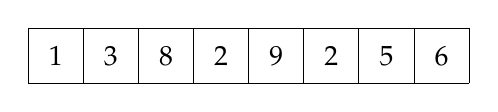
\begin{tikzpicture}[scale=0.7]
\draw (0,0) grid (8,1);
\node at (0.5,0.5) {$1$};
\node at (1.5,0.5) {$3$};
\node at (2.5,0.5) {$8$};
\node at (3.5,0.5) {$2$};
\node at (4.5,0.5) {$9$};
\node at (5.5,0.5) {$2$};
\node at (6.5,0.5) {$5$};
\node at (7.5,0.5) {$6$};
\end{tikzpicture}
\end{center}
will be as follows after sorting:
\begin{center}
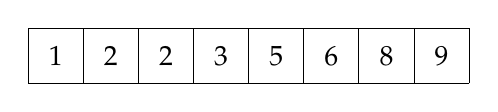
\begin{tikzpicture}[scale=0.7]
\draw (0,0) grid (8,1);
\node at (0.5,0.5) {$1$};
\node at (1.5,0.5) {$2$};
\node at (2.5,0.5) {$2$};
\node at (3.5,0.5) {$3$};
\node at (4.5,0.5) {$5$};
\node at (5.5,0.5) {$6$};
\node at (6.5,0.5) {$8$};
\node at (7.5,0.5) {$9$};
\end{tikzpicture}
\end{center}
\end{exmp}
\section{Properties of Sorting Algorithms}
\subsection{Types of Sorting Algorithms}
There are two broad types of sorting algorithms: integer sorts and comparison sorts.
\subsubsection{Comparison Sorts}
Comparison sorts compare elements at each step of the algorithm to determine if one element should be to the left or right of another element.

Comparison sorts are usually more straightforward to implement than integer sorts, but comparison sorts are limited by a lower bound of $\mathcal{O}(n\log{n})$, meaning that, on average, comparison sorts cannot be faster than $\mathcal{O}(n\log{n})$.
\subsubsection{Integer Sorts}
Integer sorts are sometimes called counting sorts (though there is a specific integer sort algorithm called counting sort). Integer sorts do not make comparisons. Integer sorts determine for each element $x$ - how many elements are less than $x$. For example, if there are $14$ elements that are less than $x$, then $x$ will be placed in the $15^{th}$ slot. This information is used to place each element into the correct slot immediately, so there is no need to rearrange lists.
\subsection{Stability}
Stable sorting algorithms maintain the relative order of records with equal keys (i.e. values). That is, a sorting algorithm is stable if whenever there are two records $R$ and $S$ with the same key and with $R$ appearing before $S$ in the original list, $R$ will appear before $S$ in the sorted list.
\subsection{Adaptability}
It means whether or not the presortedness of the input affects the running time. Algorithms that take this into account are known to be adaptive.
\subsection{Memory Usage}
Some sorting algorithms are called "in-place". Strictly, an in-place sort needs only $\mathcal{O}(1)$ memory beyond the items being sorted; sometimes $\mathcal{O}(\log{n})$ additional memory is considered "in-place".
\subsection{Computational Complexity}
For typical serial sorting algorithms good behaviour is $\mathcal{O}(n\log{n})$, with parallel sort in $\mathcal{O}(\log^{2}{n})$, and bad behaviour is $\mathcal{O}(n^2)$.
\section{Common \texorpdfstring{$\mathcal{O}(n^2)$}{O(n square)} Algorithms}
These algorithms are arguably easy to implement but generally not used due to high time complexity.
\subsection{Bubble Sort}
Bubble sort is a simple sorting algorithm. The algorithm starts at the beginning of the data set. It compares the first two elements, and if the first is greater than the second, it swaps them. It continues doing this for each pair of adjacent elements to the end of the data set. It then starts again with the first two elements, repeating until no swaps have occurred on the last pass. It is rarely used to sort large, unordered data sets.
\hfill\break
\begin{center}
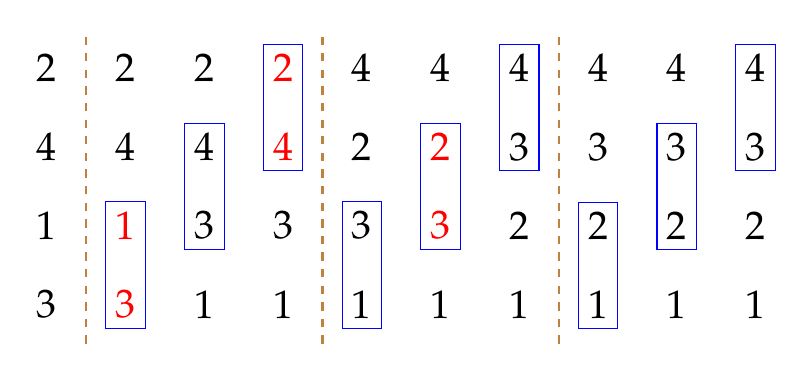
\begin{tikzpicture}[rotate = 90, swap/.style = {dashed, thick},
  inv/.style = {blue, rectangle, draw, inner sep = 0pt, outer sep = 0pt},
  ele/.style = {font = \Large},
  pass/.style = {brown, thick, dashed}]
  \foreach \e [count = \ei] in {3,1,4,2} {
    \node (1\e) [ele] at (\ei, 1) {$\e$};
  }

  \draw [pass] (0.5, 0.5) to (4.5,0.5);

  \foreach \e [count = \ei] in {3,1,4,2} {
    \node (1\e) [ele] at (\ei, 0) {\ifthenelse{\e = 3 \OR \e = 1}{\textcolor{red}{$\e$}}{$\e$}};
  }
  \begin{pgfonlayer}{background}
    \node () [inv, fit = (13) (11)] {};
  \end{pgfonlayer}

  \foreach \e [count = \ei] in {1,3,4,2} {
    \node (2\e) [ele] at (\ei, -1) {$\e$};
  }
  \begin{pgfonlayer}{background}
    \node () [inv, fit = (23) (24)] {};
  \end{pgfonlayer}

  \foreach \e [count = \ei] in {1,3,4,2} {
    \node (3\e) [ele] at (\ei, -2) {\ifthenelse{\e = 4 \OR \e = 2}{\textcolor{red}{$\e$}}{$\e$}};
  }
  \begin{pgfonlayer}{background}
    \node () [inv, fit = (34) (32)] {};
  \end{pgfonlayer}

  \draw [pass] (0.5, -2.5) to (4.5,-2.5);

  % the second pass
  \foreach \e [count = \ei] in {1,3,2,4} {
    \node (4\e) [ele] at (\ei, -3) {$\e$};
  }
  \begin{pgfonlayer}{background}
    \node () [inv, fit = (41) (43)] {};
  \end{pgfonlayer}

  \foreach \e [count = \ei] in {1,3,2,4} {
    \node (5\e) [ele] at (\ei, -4) {\ifthenelse{\e = 3 \OR \e = 2}{\textcolor{red}{$\e$}}{$\e$}};
  }
  \begin{pgfonlayer}{background}
    \node () [inv, fit = (53) (52)] {};
  \end{pgfonlayer}

  \foreach \e [count = \ei] in {1,2,3,4} {
    \node (6\e) [ele] at (\ei, -5) {$\e$};
  }
  \begin{pgfonlayer}{background}
    \node () [inv, fit = (63) (64)] {};
  \end{pgfonlayer}

  \draw [pass] (0.5, -5.5) to (4.5,-5.5);

  \foreach \e [count = \ei] in {1,2,3,4} {
    \node (7\e) [ele] at (\ei, -6) {$\e$};
  }
  \begin{pgfonlayer}{background}
    \node () [inv, fit = (71) (72)] {};
  \end{pgfonlayer}

  \foreach \e [count = \ei] in {1,2,3,4} {
    \node (8\e) [ele] at (\ei, -7) {$\e$};
  }
  \begin{pgfonlayer}{background}
    \node () [inv, fit = (82) (83)] {};
  \end{pgfonlayer}

  \foreach \e [count = \ei] in {1,2,3,4} {
    \node (9\e) [ele] at (\ei, -8) {$\e$};
  }
  \begin{pgfonlayer}{background}
    \node () [inv, fit = (93) (94)] {};
  \end{pgfonlayer}
\end{tikzpicture}

Example of Bubble Sort
\end{center}
\subsection{Insertion Sort}
Insertion sort is a simple sorting algorithm that is relatively efficient for small lists and mostly sorted lists, and is often used as part of more sophisticated algorithms. It works by taking elements from the list one by one and inserting them in their correct position into a new sorted list. In arrays, the new list and the remaining elements can share the array's space, but insertion is expensive, requiring shifting all following elements over by one.

\begin{figure}[htbp]
  \centering
  \includesvg[scale=0.5]{Insertion.svg}

  Insertion Sort Example
\end{figure}

\section{Common \texorpdfstring{$\mathcal{O}(n\log{n})$}{O(nlog(n))} Algorithms}
\subsection{Merge Sort}
Merge sort sorts a subarray \texttt{array}$[a \ldots b]$ as follows:

\begin{enumerate}
\item If $a=b$, do not do anything, because the subarray is already sorted.
\item Calculate the position of the middle element: $k=\lfloor (a+b)/2 \rfloor$.
\item Recursively sort the subarray \texttt{array}$[a \ldots k]$.
\item Recursively sort the subarray \texttt{array}$[k+1 \ldots b]$.
\item \emph{Merge} the sorted subarrays \texttt{array}$[a \ldots k]$ and
\texttt{array}$[k+1 \ldots b]$
into a sorted subarray \texttt{array}$[a \ldots b]$.
\end{enumerate}

Merge sort is an efficient algorithm, because it
halves the size of the subarray at each step.
The recursion consists of $\mathcal{O}(\log n)$ levels,
and processing each level takes $O(n)$ time.
Merging the subarrays \texttt{array}$[a \ldots k]$ and \texttt{array}$[k+1 \ldots b]$
is possible in linear time, because they are already sorted.

For example, consider sorting the following array:
\begin{center}
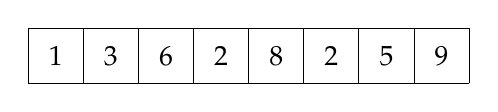
\begin{tikzpicture}[scale=0.7]
\draw (0,0) grid (8,1);
\node at (0.5,0.5) {$1$};
\node at (1.5,0.5) {$3$};
\node at (2.5,0.5) {$6$};
\node at (3.5,0.5) {$2$};
\node at (4.5,0.5) {$8$};
\node at (5.5,0.5) {$2$};
\node at (6.5,0.5) {$5$};
\node at (7.5,0.5) {$9$};
\end{tikzpicture}

\vspace{5mm}

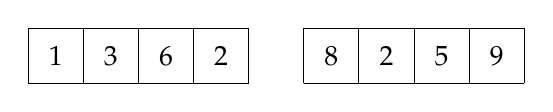
\begin{tikzpicture}[scale=0.7]
\draw (0,0) grid (4,1);
\draw (5,0) grid (9,1);

\node at (0.5,0.5) {$1$};
\node at (1.5,0.5) {$3$};
\node at (2.5,0.5) {$6$};
\node at (3.5,0.5) {$2$};

\node at (5.5,0.5) {$8$};
\node at (6.5,0.5) {$2$};
\node at (7.5,0.5) {$5$};
\node at (8.5,0.5) {$9$};
\end{tikzpicture}

\vspace{5mm}

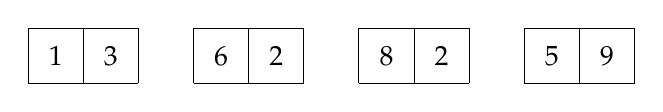
\begin{tikzpicture}[scale=0.7]
\draw (0,0) grid (2,1);
\draw (3,0) grid (5,1);
\draw (6,0) grid (8,1);
\draw (9,0) grid (11,1);

\node at (0.5,0.5) {$1$};
\node at (1.5,0.5) {$3$};
\node at (3.5,0.5) {$6$};
\node at (4.5,0.5) {$2$};

\node at (6.5,0.5) {$8$};
\node at (7.5,0.5) {$2$};
\node at (9.5,0.5) {$5$};
\node at (10.5,0.5) {$9$};
\end{tikzpicture}

\vspace{5mm}

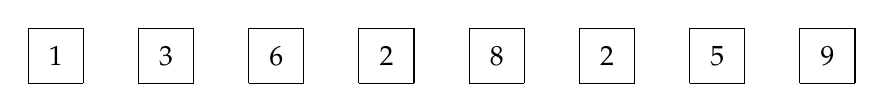
\begin{tikzpicture}[scale=0.7]
\draw (0,0) grid (1,1);
\draw (2,0) grid (3,1);
\draw (4,0) grid (5,1);
\draw (6,0) grid (7,1);
\draw (8,0) grid (9,1);
\draw (10,0) grid (11,1);
\draw (12,0) grid (13,1);
\draw (14,0) grid (15,1);

\node at (0.5,0.5) {$1$};
\node at (2.5,0.5) {$3$};
\node at (4.5,0.5) {$6$};
\node at (6.5,0.5) {$2$};

\node at (8.5,0.5) {$8$};
\node at (10.5,0.5) {$2$};
\node at (12.5,0.5) {$5$};
\node at (14.5,0.5) {$9$};
\end{tikzpicture}

\vspace{5mm}
MERGING BEGINS
\vspace{5mm}

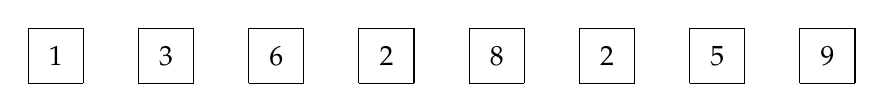
\begin{tikzpicture}[scale=0.7]
\draw (0,0) grid (1,1);
\draw (2,0) grid (3,1);
\draw (4,0) grid (5,1);
\draw (6,0) grid (7,1);
\draw (8,0) grid (9,1);
\draw (10,0) grid (11,1);
\draw (12,0) grid (13,1);
\draw (14,0) grid (15,1);

\node at (0.5,0.5) {$1$};
\node at (2.5,0.5) {$3$};
\node at (4.5,0.5) {$6$};
\node at (6.5,0.5) {$2$};

\node at (8.5,0.5) {$8$};
\node at (10.5,0.5) {$2$};
\node at (12.5,0.5) {$5$};
\node at (14.5,0.5) {$9$};
\end{tikzpicture}

\vspace{5mm}

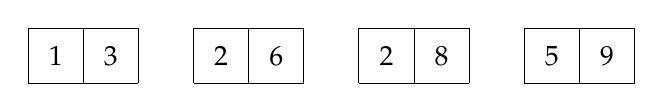
\begin{tikzpicture}[scale=0.7]
\draw (0,0) grid (2,1);
\draw (3,0) grid (5,1);
\draw (6,0) grid (8,1);
\draw (9,0) grid (11,1);

\node at (0.5,0.5) {$1$};
\node at (1.5,0.5) {$3$};
\node at (3.5,0.5) {$2$};
\node at (4.5,0.5) {$6$};

\node at (6.5,0.5) {$2$};
\node at (7.5,0.5) {$8$};
\node at (9.5,0.5) {$5$};
\node at (10.5,0.5) {$9$};
\end{tikzpicture}

\vspace{5mm}

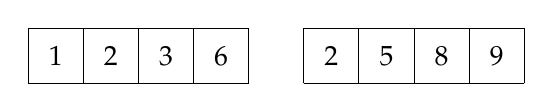
\begin{tikzpicture}[scale=0.7]
\draw (0,0) grid (4,1);
\draw (5,0) grid (9,1);

\node at (0.5,0.5) {$1$};
\node at (1.5,0.5) {$2$};
\node at (2.5,0.5) {$3$};
\node at (3.5,0.5) {$6$};

\node at (5.5,0.5) {$2$};
\node at (6.5,0.5) {$5$};
\node at (7.5,0.5) {$8$};
\node at (8.5,0.5) {$9$};
\end{tikzpicture}

\vspace{5mm}

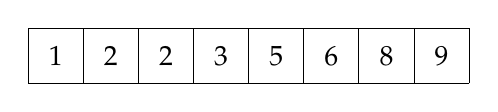
\begin{tikzpicture}[scale=0.7]
\draw (0,0) grid (8,1);
\node at (0.5,0.5) {$1$};
\node at (1.5,0.5) {$2$};
\node at (2.5,0.5) {$2$};
\node at (3.5,0.5) {$3$};
\node at (4.5,0.5) {$5$};
\node at (5.5,0.5) {$6$};
\node at (6.5,0.5) {$8$};
\node at (7.5,0.5) {$9$};
\end{tikzpicture}
\end{center}

\subsection{Quick Sort}

Quicksort uses divide and conquer to sort an array. Divide and conquer is a technique used for breaking algorithms down into subproblems, solving the subproblems, and then combining the results back together to solve the original problem. It can be helpful to think of this method as divide, conquer, and combine.

Here are the divide, conquer, and combine steps that quicksort uses:

\textbf{Divide:}

\begin{enumerate}
\item Pick a pivot element, \texttt{$A[q]$}. Picking a good pivot is the key for a fast implementation of quicksort; however, it is difficult to determine what a good pivot might be.
\item Partition, or rearrange, the array into two subarrays: \texttt{$A[p,...,q-1]$} such that all elements are less than \texttt{$A[q]$}, and \texttt{$A[q+1,...,r]$} such that all elements are greater than or equal to \texttt{$A[q]$}.
\end{enumerate}
\newpage

\textbf{Conquer:}

\begin{enumerate}
\item Sort the subarrays \texttt{$A[p,...,q-1]$} and \texttt{$A[q+1,...,r]$} recursively with quicksort.
\end{enumerate}

\textbf{Combine:}

\begin{enumerate}
\item No work is needed to combine the arrays because they are already sorted.
\end{enumerate}

\begin{figure}[htbp]
  \centering
  \includesvg[scale=0.8]{Quicksort.svg}

  Quicksort Example
\end{figure}
\newpage

\subsection{Heap Sort}

Heapsort is a much more efficient version of selection sort. It also works by determining the largest (or smallest) element of the list, placing that at the end (or beginning) of the list, then continuing with the rest of the list, but accomplishes this task efficiently by using a data structure called a heap, a special type of binary tree.

\subsection{Counting Sort}

Counting sort assumes that each of the $n$ input elements in a list has a key value ranging from $0$ to $k$, for some integer $k$. For each element in the list, counting sort determines the number of elements that are less than it. Counting sort can use this information to place the element directly into the correct slot of the output array.

Counting sort uses three lists: the input list, \texttt{$A[0,1,...,n]$}, the output list, \texttt{$B[0,1,...,n]$}, and a list that serves as temporary memory, \texttt{$C[0,1,...,k]$}. Note that $A$ and $B$ have $n$ slots (a slot for each element), while $C$ contains $k$ slots (a slot for each key value).

\section{Comparison of Sorting Algorithms}


\begin{table}[!ht]
\makebox[\linewidth]{
\begin{tabularx}{7in}{|X|X|X|X|X|X|}
\hline
\textbf{Algorithm}      & \textbf{Best Case}                              & \textbf{Worst Case}                             & \textbf{Average Case}                           & \textbf{Space Usage}                  & \textbf{Stable?}                    \\ \hline
\textbf{Bubble Sort}    & \cellcolor[HTML]{67FD9A}$\mathcal{O}(n)$        & \cellcolor[HTML]{FE0000}$\mathcal{O}(n^2)$      & \cellcolor[HTML]{FE0000}$\mathcal{O}(n^2)$      & \cellcolor[HTML]{67FD9A}$\mathcal{O}(1)$   & \cellcolor[HTML]{67FD9A}Yes         \\ \hline
\textbf{Insertion Sort} & \cellcolor[HTML]{67FD9A}$\mathcal{O}(n)$        & \cellcolor[HTML]{FE0000}$\mathcal{O}(n^2)$      & \cellcolor[HTML]{FE0000}$\mathcal{O}(n^2)$      & \cellcolor[HTML]{67FD9A}$\mathcal{O}(1)$   & \cellcolor[HTML]{67FD9A}Yes         \\ \hline
\textbf{Merge Sort}     & \cellcolor[HTML]{FFCC67}$\mathcal{O}(n\log{n})$ & \cellcolor[HTML]{67FD9A}$\mathcal{O}(n\log{n})$ & \cellcolor[HTML]{67FD9A}$\mathcal{O}(n\log{n})$ & \cellcolor[HTML]{FFCC67}$\mathcal{O}(n)$   & \cellcolor[HTML]{67FD9A}Yes         \\ \hline
\textbf{Quicksort}      & \cellcolor[HTML]{FFCC67}$\mathcal{O}(n\log{n})$ & \cellcolor[HTML]{FE0000}$\mathcal{O}(n^2)$      & \cellcolor[HTML]{67FD9A}$\mathcal{O}(n\log{n})$ & \cellcolor[HTML]{FFCC67}$\mathcal{O}(n)$   & \cellcolor[HTML]{FFCC67}Usually Not \\ \hline
\textbf{Heapsort}       & \cellcolor[HTML]{FFCC67}$\mathcal{O}(n\log{n})$ & \cellcolor[HTML]{67FD9A}$\mathcal{O}(n\log{n})$ & \cellcolor[HTML]{67FD9A}$\mathcal{O}(n\log{n})$ & \cellcolor[HTML]{67FD9A}$\mathcal{O}(1)$   & \cellcolor[HTML]{FE0000}No          \\ \hline
\textbf{Counting Sort}  & \cellcolor[HTML]{67FD9A}$\mathcal{O}(k+n)$      & \cellcolor[HTML]{67FD9A}$\mathcal{O}(k+n)$      & \cellcolor[HTML]{67FD9A}$\mathcal{O}(k+n)$      & \cellcolor[HTML]{FFCC67}$\mathcal{O}(k+n)$ & \cellcolor[HTML]{67FD9A}Yes         \\ \hline
\end{tabularx}
}
\end{table}

\section{Sorting in C++}

The C++ standard library contains
the function \texttt{sort} that can be easily used for
sorting arrays and other data structures.

There are many benefits in using a library function.
First, it saves time because there is no need to
implement the function.
Second, the library implementation is
certainly correct and efficient: it is not probable
that a home-made sorting function would be better.

In this section we will see how to use the
C++ \texttt{sort} function.
The following code sorts
a vector in increasing order:
\begin{lstlisting}
vector<int> v = {4,2,5,3,5,8,3};
sort(v.begin(),v.end());
\end{lstlisting}
After the sorting, the contents of the
vector will be
$[2,3,3,4,5,5,8]$.
The default sorting order is increasing,
but a reverse order is possible as follows:
\begin{lstlisting}
sort(v.rbegin(),v.rend());
\end{lstlisting}
An ordinary array can be sorted as follows:
\begin{lstlisting}
int n = 7; // array size
int a[] = {4,2,5,3,5,8,3};
sort(a, a+n);
\end{lstlisting}
The following code sorts the string \texttt{s}:
\begin{lstlisting}
string s = "monkey";
sort(s.begin(), s.end());
\end{lstlisting}
Sorting a string means that the characters
of the string are sorted.
For example, the string ''monkey'' becomes ''ekmnoy''.

Integer containers can be sorted in decreasing order as follows:

\begin{lstlisting}
int n = 7; // array size
int a[] = {4,2,5,3,5,8,3};
sort(a, a+n, greater<int>());// greater<int>() as third parameter
// final array is int a[] = {8,5,5,4,3,3,2};
\end{lstlisting}


\chapter{Bit Manipulation}
\section{Tricks}
\subsection{Multiply and divide by \texorpdfstring{$2^i$}{2**i}}
\begin{lstlisting}
n = n << i;   // Multiply n with 2^i
n = n >> 1;   // Divide n by 2^i
\end{lstlisting}
\subsection{Checking if a number is odd or even}
\begin{lstlisting}
if (num & 1)
   cout << "ODD";
else
   cout << "EVEN";
\end{lstlisting}
\subsection{Swapping of 2 numbers using XOR}
This method is fast and doesn’t require the use of 3rd variable.
\begin{lstlisting}
a ^= b;
b ^= a;
a ^= b;
\end{lstlisting}
\newpage
\subsection{Compute XOR from 1 to \texorpdfstring{$n$}{n} (direct method)}
\begin{algorithm}
%\DontPrintSemicolon % Some LaTeX compilers require you to use \dontprintsemicolon    instead
\KwIn{$n$}
\KwOut{XOR of all numbers from $1$ to $n$}
Find the remainder of n by moduling it with 4.\\
Check, \linebreak
%\renewcommand{\labelenumi}{(\Roman{enumi})}
%\begin{enumerate}[noitemsep,nolistsep]
%\item
 (I) If rem = 0, then xor will be same as n.
\linebreak
%\item
(II) If rem = 1, then xor will be 1.
\linebreak
%\item
(II) If rem = 1, then xor will be 1.
\linebreak
%\item
(II) If rem = 3 ,then xor will be 0.
%\end{enumerate}
\caption{Compute XOR of numbers from $1$ to $n$}
\label{algo:b}
\end{algorithm}
\begin{lstlisting}
int computeXOR(int n)
{
    if (n % 4 == 0)
        return n;
    if (n % 4 == 1)
        return 1;
    if (n % 4 == 2)
        return n + 1;
    else
        return 0;
}
\end{lstlisting}
\subsubsection{How does this work?}
When we do XOR of numbers, we get 0 as XOR value just before a multiple of 4. This keeps repeating before every multiple of 4.
\begin{lstlisting}
Number Binary-Repr  XOR-from-1-to-n
1         1           [0001]
2        10           [0011]
3        11           [0000]  <----- We get a 0
4       100           [0100]  <----- Equals to n
5       101           [0001]
6       110           [0111]
7       111           [0000]  <----- We get 0
8      1000           [1000]  <----- Equals to n
9      1001           [0001]
10     1010           [1011]
11     1011           [0000] <------ We get 0
12     1100           [1100] <------ Equals to n
\end{lstlisting}
\newpage
\subsection{Check if a number is a power of \texorpdfstring{$2$}{2}}
\begin{lstlisting}
bool poweroftwo(int x)
{
    return x & (x-1) == 0;
}
\end{lstlisting}
\subsection{Change case of English alphabet}
\begin{lstlisting}
ch |= ' '; //Upper to Lower
ch &= '_' ; //Lower to Upper
\end{lstlisting}
\subsection{Find \texorpdfstring{$\log_2 x$}{log} of integer}
\begin{lstlisting}
int logarithm(int x)
{
    int res = 0;
    while (x >>= 1)
        res++;
    return res;
}
\end{lstlisting}
\section{Bit Shift}
The left bit shift $x \verb|<<| k$ appends $k$
zero bits to the number,
and the right bit shift $x \verb|>>| k$
removes the $k$ last bits from the number.

Note that $x \verb|<<| k$
corresponds to multiplying $x$ by $2^k$,
and $x \verb|>>| k$
corresponds to dividing $x$ by $2^k$
rounded down to an integer
\subsection{Application}
\subsubsection{Check if $k^{th}$ bit is set}
The $k$th bit of a number is one
exactly when $x$ \and $(1 \verb|<<| k)$ is not zero.
The following code prints the bit representation
of an \texttt{int} number $x$:

\begin{lstlisting}
for (int i = 31; i >= 0; i--)
{
    if (x&(1<<i)) cout << "1"; //check if ith bit is 1
    else cout << "0";
}
\end{lstlisting}
\subsubsection{Set the $k^{th}$ bit}
\begin{lstlisting}
x |= (1 < < k) //sets the kth bit of x to one
\end{lstlisting}
\subsubsection{Unset the $k^{th}$ bit}
\begin{lstlisting}
x &= ~(1 << k) //unsets the kth bit of x to zero
\end{lstlisting}
\subsubsection{Invert the $k^{th}$ bit}
\begin{lstlisting}
x ^= (1 << k) //Inverts the kth bit of x
\end{lstlisting}
\subsubsection{To get the Least Significant Bit}
\begin{lstlisting}
T = (S & (-S))
//T is a power of two with only one bit set which is the LSB.
\end{lstlisting}
\subsubsection{To turn on all bits of a number}
\begin{lstlisting}
~(x & 0) //x&0 is 0 and ~ inverts all bits to 1
\end{lstlisting}
\subsubsection{To turn on all bits till $n$}
\begin{lstlisting}
S = (1 << n) - 1 //in case n =3 , s = 7 = 8-1
\end{lstlisting}
\subsubsection{Get $n \mod d$ where d is a power of 2}
\begin{lstlisting}
// This function will return n % d.
// d must be one of: 1, 2, 4, 8, 16, 32, ...
unsigned int getModulo(unsigned int n, unsigned int d)
{
return ( n & (d - 1) );
}
\end{lstlisting}
\subsubsection{Trivia}
The formula $x$ \& $(x-1)$ sets the last
one bit of $x$ to zero.
The formula $x$ | $(x-1)$
inverts all the bits after the last one bit.
\section{C++ Special Functions}
The g++ compiler provides the following
functions for counting bits:

\begin{itemize}
\item
$\texttt{\_\_builtin\_clz}(x)$:
the number of zeros at the beginning of the number
\item
$\texttt{\_\_builtin\_ctz}(x)$:
the number of zeros at the end of the number
\item
$\texttt{\_\_builtin\_popcount}(x)$:
the number of ones in the number
\item
$\texttt{\_\_builtin\_parity}(x)$:
the parity (even or odd) of the number of ones
\end{itemize}
\begin{samepage}

The functions can be used as follows:
\begin{lstlisting}
int x = 5328; // 00000000000000000001010011010000
cout << __builtin_clz(x) << "\n"; // 19
cout << __builtin_ctz(x) << "\n"; // 4
cout << __builtin_popcount(x) << "\n"; // 5
cout << __builtin_parity(x) << "\n"; // 1
\end{lstlisting}
\end{samepage}

While the above functions only support \texttt{int} numbers,
there are also \texttt{long long} versions of
the functions available with the suffix \texttt{ll} like $\texttt{\_\_builtin\_popcountll}(x)$.
\section{Set Representation}
Every subset of a set
$\{0,1,2,\ldots,n-1\}$
can be represented as an $n$ bit integer
whose one bits indicate which
elements belong to the subset.
This is an efficient way to represent sets,
because every element requires only one bit of memory,
and set operations can be implemented as bit operations.

For example, since \texttt{int} is a 32-bit type,
an \texttt{int} number can represent any subset
of the set $\{0,1,2,\ldots,31\}$.
The bit representation of the set $\{1,3,4,8\}$ is
\[00000000000000000000000100011010,\]
which corresponds to the number $2^8+2^4+2^3+2^1=282$.

\subsection{Set implementation}

The following code declares an \texttt{int}
variable $x$ that can contain
a subset of $\{0,1,2,\ldots,31\}$.
After this, the code adds the elements 1, 3, 4 and 8
to the set and prints the size of the set.
\begin{lstlisting}
int x = 0;
x |= (1<<1);
x |= (1<<3);
x |= (1<<4);
x |= (1<<8);
cout << __builtin_popcount(x) << "\n"; // 4
\end{lstlisting}
Then, the following code prints all
elements that belong to the set:
\begin{lstlisting}
for (int i = 0; i < 32; i++) {
    if (x&(1<<i)) cout << i << " ";
}
// output: 1 3 4 8
\end{lstlisting}

\section{Example Problems}
\subsection{Counting Grids with Black Corners}
\begin{problem}
Given an $n \times n$ grid whose
each square is either black (1) or white (0),
calculate the number of subgrids
whose all corners are black.
\end{problem}
\begin{exmp}
For example, the grid
\begin{center}
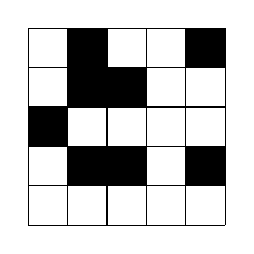
\begin{tikzpicture}[scale=0.5]
\fill[black] (1,1) rectangle (2,2);
\fill[black] (1,4) rectangle (2,5);
\fill[black] (4,1) rectangle (5,2);
\fill[black] (4,4) rectangle (5,5);
\fill[black] (1,3) rectangle (2,4);
\fill[black] (2,3) rectangle (3,4);
\fill[black] (2,1) rectangle (3,2);
\fill[black] (0,2) rectangle (1,3);
\draw (0,0) grid (5,5);
\end{tikzpicture}
\end{center}
contains two such subgrids:
\begin{center}
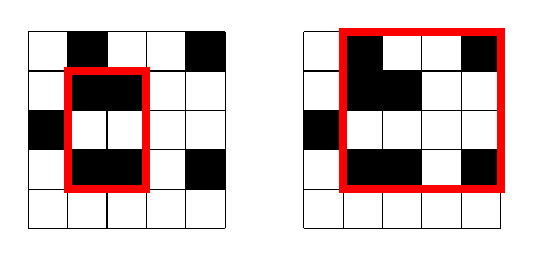
\begin{tikzpicture}[scale=0.5]
\fill[black] (1,1) rectangle (2,2);
\fill[black] (1,4) rectangle (2,5);
\fill[black] (4,1) rectangle (5,2);
\fill[black] (4,4) rectangle (5,5);
\fill[black] (1,3) rectangle (2,4);
\fill[black] (2,3) rectangle (3,4);
\fill[black] (2,1) rectangle (3,2);
\fill[black] (0,2) rectangle (1,3);
\draw (0,0) grid (5,5);

\fill[black] (7+1,1) rectangle (7+2,2);
\fill[black] (7+1,4) rectangle (7+2,5);
\fill[black] (7+4,1) rectangle (7+5,2);
\fill[black] (7+4,4) rectangle (7+5,5);
\fill[black] (7+1,3) rectangle (7+2,4);
\fill[black] (7+2,3) rectangle (7+3,4);
\fill[black] (7+2,1) rectangle (7+3,2);
\fill[black] (7+0,2) rectangle (7+1,3);
\draw (7+0,0) grid (7+5,5);

\draw[color=red,line width=1mm] (1,1) rectangle (3,4);
\draw[color=red,line width=1mm] (7+1,1) rectangle (7+5,5);
\end{tikzpicture}
\end{center}
\end{exmp}
\begin{tcolorbox}[title=Solution]
\hfill\break
Naive Solution of time complexity $\mathcal{O}(n^3)$:

Go through all $O(n^2)$ pairs of rows and for each pair
$(a,b)$ calculate the number of columns that contain a black
square in both rows in $O(n)$ time.
The following code assumes that $\texttt{color}[y][x]$
denotes the color in row $y$ and column $x$:
\begin{lstlisting}
int count = 0;
for (int i = 0; i < n; i++) {
    if (color[a][i] == 1 && color[b][i] == 1) count++;
}
\end{lstlisting}
Then, those columns
account for $\texttt{count}(\texttt{count}-1)/2$ subgrids with black corners,
because we can choose any two of them to form a subgrid.
\end{tcolorbox}
\newpage
\begin{tcolorbox}[title=Solution]
\hfill\break
Optimized solution:

Divide the grid into blocks
of columns such that each block consists of $N$
consecutive columns. Then, each row is stored as
a list of $N$-bit numbers that describe the colors
of the squares. Now we can process $N$ columns at the same time
using bit operations. In the following code,
$\texttt{color}[y][k]$ represents
a block of $N$ colors as bits.
\begin{lstlisting}
int count = 0;
for (int i = 0; i <= n/N; i++) {
    count += __builtin_popcount(color[a][i]&color[b][i]);
}
\end{lstlisting}
Time Complexity is $O(n^3/N)$ time.
\end{tcolorbox}

\chapter{Brute-Force Algorithms}


\section{Generating Subsets}

\begin{problem}
Print all the subsets of a set of size $n$.
\end{problem}

\begin{exmp}
For example, the subsets of $\{0,1,2\}$ are
$\emptyset$, $\{0\}$, $\{1\}$, $\{2\}$, $\{0,1\}$,
$\{0,2\}$, $\{1,2\}$ and $\{0,1,2\}$.
\end{exmp}

\begin{tcolorbox}[title=Solution]

We can use the bit representation of numbers to generate subsets.

Let's say, set $s$ has $n$ elements. We will use the bits of numbers to show the presence of element in set. If $x^{th}$ bit in number is SET, then $x^{th}$ element in $s$ is present in current subset. We will loop from $0$ to $2^n - 1$, and for each number, we will check among the first $n$ bits, the SET bits in it and take corresponding elements. In each iteration, we will have one subset.

\begin{lstlisting}
int arr[n]; //array of n elements
for(int j = 0; j< (1 << n); j++)
{   // (1<<n) is equal to 2^n - 1
    for(int i = 0; i<n; i++)
    {   //checking first n bits
        if(j&(1<<i))
        {   //print the corresponding element
            //first subset is always null set
            cout << arr[i] << " ";
        }
    }
    cout << "\n";
}
\end{lstlisting}
The time complexity is $\mathcal{O}(n2^n)$ which is exponential.
\end{tcolorbox}
\section{Generating Permutations}
\begin{problem}
Print all the permutations of a set of size $n$.
\end{problem}
\begin{exmp}
For example, the permutations of $\{0,1,2\}$ are
$(0,1,2)$, $(0,2,1)$, $(1,0,2)$, $(1,2,0)$,
$(2,0,1)$ and $(2,1,0)$.
\end{exmp}
\begin{tcolorbox}[title=Solution]

We can use the built-in C++ function \texttt{next\textunderscore permutation} which rearranges the array into the next lexicographically greater permutation. It returns $1$ if this is possible and $0$ otherwise.

\begin{lstlisting}
int arr[n]; //array of n elements
do
{//we use do while loop to also print the original array itself
    for(int i : arr)
    {
        cout << i << " ";
    }
    cout << "\n";
}
while(next_permutation(arr, arr+n));
\end{lstlisting}

\end{tcolorbox}


\chapter{Searching}

\section{Binary Search}

Binary search is the most popular search algorithm. It is efficient and also one of the most commonly used techniques that is used to solve problems.

We will explain this technique using a problem

\begin{problem}
Given a sorted array $A[]$ of $n$ elements, write a function to search a given element $x$ in $A[]$.
\end{problem}

\textbf{Constraints:} The array contains about $10^{10}$ elements. Each element is less than $10^9$

\begin{tcolorbox}[breakable, title=Solution]
\textbf{Naive Approach:} A simple approach is to do a linear search(checking every element). The time complexity would be $\mathcal{O}(n)$
\tcblower
\textbf{Binary Search:} Search a sorted array by repeatedly dividing the search interval in half. Begin with an interval covering the whole array. If the value of the search key is less than the item in the middle of the interval, narrow the interval to the lower half. Otherwise narrow it to the upper half. Repeatedly check until the value is found or the interval is empty.

Since we are halving the array at each step, the time complexity becomes $\mathcal{O}(\log{n})$

\includesvg[scale=0.5]{Binary_search.svg}

\begin{lstlisting}
int search(int low,int high,int key)
{
   while(low<=high)
   {
     int mid=(low+high)/2;
     if(a[mid]<key)
     {
         low=mid+1; //search upper half
     }
     else if(a[mid]>key)
     {
         high=mid-1; //search lower half
     }
     else
     {
         return mid; //key found
     }
   }
   return -1;        //key not found
 }
\end{lstlisting}
\end{tcolorbox}
\newpage
\subsection{Binary Search in C++ STL}

C++ STL has built-in binary search algorithms for a container

\begin{itemize}
    \item \texttt{binary\textunderscore search()} : it returns true if value is present in array and false otherwise.
    \item \texttt{lower\textunderscore bound()} : it returns an iterator pointing to the first element in the array which is greater than or equal to value.
    \item \texttt{upper\textunderscore bound()} : it returns an iterator pointing to the first element in the array which is greater than value.
\end{itemize}

\section{Two Pointer Technique}

Two pointer is really an easy and effective technique which is typically used for searching pairs in a sorted array. Binary search is a kind of optimisation on the number of trials taken to reach the optimal position and so is the two pointer technique. The approach relies on the sequence following one specific property on which our pointers can move.

We will explain this technique using an example problem.

\begin{problem}
Given a sorted array $A$, having $N$ integers. You need to find any pair$(i,j)$ having sum as given number $X$.
\end{problem}

\textbf{Constraints:} Array $A$ contains about $10^5$ integers with each having values around $10^9$.

\begin{tcolorbox}[breakable, title=Solution]
\textbf{Naive Solution:} We iterate over every $i$ and $j$ and find out the pair which sums up to $X$. This approach is to slow because it leads to a time complexity of $\mathcal{O}(n^2)$
\tcblower
\textbf{2 Pointer Technique:} Now let’s see how the two pointer technique works. We take two pointers, one representing the first element and other representing the last element of the array, and then we add the values kept at both the pointers. If their sum is smaller than X then we shift the left pointer to right or if their sum is greater than X then we shift the right pointer to left, in order to get closer to the sum. We keep moving the pointers until we get the sum as $X$ or the left pointer meets the right pointer and we don't find the value $X$.

The time complexity is $\mathcal{O}(n)$ if the array is already sorted.
\newpage
\begin{lstlisting}
bool isPairSum(A[], N, X) 
{
    int i = 0; //left pointer 
    int j = N - 1; //right pointer
  
    while (i < j) 
    { 
        // If we find a pair 
        if (A[i] + A[j] == X) 
            return true; 

        // If sum of elements at current 
        // pointers is less, we move towards 
        // higher values by doing i++ 
        else if (A[i] + A[j] < X) 
            i++; 
  
        // If sum of elements at current 
        // pointers is more, we move towards 
        // lower values by doing i++ 
        else
            j--; 
    } 
    return false; //i crosses j
}
\end{lstlisting}
\end{tcolorbox}

\section{Sliding window minimum}

A \key{sliding window} is a constant-size subarray
that moves from left to right through the array.
At each window position,
we want to calculate some information
about the elements inside the window.
In this section, we focus on the problem
of maintaining the \key{sliding window minimum},
which means that
we should report the smallest value inside each window.

The sliding window minimum can be calculated
using a similar idea that we used to calculate
the nearest smaller elements.
We maintain a queue
where each element is larger than
the previous element,
and the first element
always corresponds to the minimum element inside the window.
After each window move,
we remove elements from the end of the queue
until the last queue element
is smaller than the new window element,
or the queue becomes empty.
We also remove the first queue element
if it is not inside the window anymore.
Finally, we add the new window element
to the end of the queue.

As an example, consider the following array:

\begin{center}
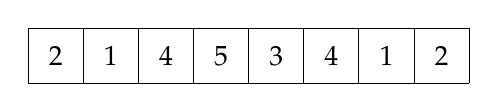
\begin{tikzpicture}[scale=0.7]
\draw (0,0) grid (8,1);

\node at (0.5,0.5) {$2$};
\node at (1.5,0.5) {$1$};
\node at (2.5,0.5) {$4$};
\node at (3.5,0.5) {$5$};
\node at (4.5,0.5) {$3$};
\node at (5.5,0.5) {$4$};
\node at (6.5,0.5) {$1$};
\node at (7.5,0.5) {$2$};
\end{tikzpicture}
\end{center}

Suppose that the size of the sliding window is 4.
At the first window position, the smallest value is 1:
\begin{center}
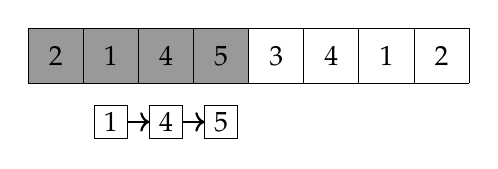
\begin{tikzpicture}[scale=0.7]
\fill[color=lightgray] (0,0) rectangle (4,1);
\draw (0,0) grid (8,1);

\node at (0.5,0.5) {$2$};
\node at (1.5,0.5) {$1$};
\node at (2.5,0.5) {$4$};
\node at (3.5,0.5) {$5$};
\node at (4.5,0.5) {$3$};
\node at (5.5,0.5) {$4$};
\node at (6.5,0.5) {$1$};
\node at (7.5,0.5) {$2$};

\draw (1.2,0.2-1.2) rectangle (1.8,0.8-1.2);
\draw (2.2,0.2-1.2) rectangle (2.8,0.8-1.2);
\draw (3.2,0.2-1.2) rectangle (3.8,0.8-1.2);

\node at (1.5,0.5-1.2) {$1$};
\node at (2.5,0.5-1.2) {$4$};
\node at (3.5,0.5-1.2) {$5$};

\draw[->,thick] (1.8,0.5-1.2) -- (2.2,0.5-1.2);
\draw[->,thick] (2.8,0.5-1.2) -- (3.2,0.5-1.2);
\end{tikzpicture}
\end{center}

Then the window moves one step right.
The new element 3 is smaller than the elements
4 and 5 in the queue, so the elements 4 and 5
are removed from the queue
and the element 3 is added to the queue.
The smallest value is still 1.
\begin{center}
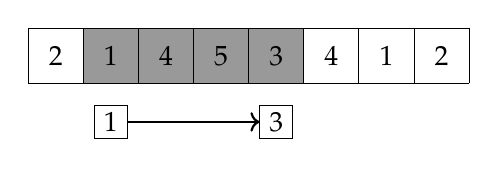
\begin{tikzpicture}[scale=0.7]
\fill[color=lightgray] (1,0) rectangle (5,1);
\draw (0,0) grid (8,1);

\node at (0.5,0.5) {$2$};
\node at (1.5,0.5) {$1$};
\node at (2.5,0.5) {$4$};
\node at (3.5,0.5) {$5$};
\node at (4.5,0.5) {$3$};
\node at (5.5,0.5) {$4$};
\node at (6.5,0.5) {$1$};
\node at (7.5,0.5) {$2$};

\draw (1.2,0.2-1.2) rectangle (1.8,0.8-1.2);
\draw (4.2,0.2-1.2) rectangle (4.8,0.8-1.2);

\node at (1.5,0.5-1.2) {$1$};
\node at (4.5,0.5-1.2) {$3$};

\draw[->,thick] (1.8,0.5-1.2) -- (4.2,0.5-1.2);
\end{tikzpicture}
\end{center}

After this, the window moves again,
and the smallest element 1
does not belong to the window anymore.
Thus, it is removed from the queue and the smallest
value is now 3. Also the new element 4
is added to the queue.
\begin{center}
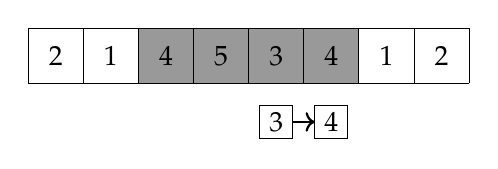
\begin{tikzpicture}[scale=0.7]
\fill[color=lightgray] (2,0) rectangle (6,1);
\draw (0,0) grid (8,1);

\node at (0.5,0.5) {$2$};
\node at (1.5,0.5) {$1$};
\node at (2.5,0.5) {$4$};
\node at (3.5,0.5) {$5$};
\node at (4.5,0.5) {$3$};
\node at (5.5,0.5) {$4$};
\node at (6.5,0.5) {$1$};
\node at (7.5,0.5) {$2$};

\draw (4.2,0.2-1.2) rectangle (4.8,0.8-1.2);
\draw (5.2,0.2-1.2) rectangle (5.8,0.8-1.2);

\node at (4.5,0.5-1.2) {$3$};
\node at (5.5,0.5-1.2) {$4$};

\draw[->,thick] (4.8,0.5-1.2) -- (5.2,0.5-1.2);
\end{tikzpicture}
\end{center}

The next new element 1 is smaller than all elements
in the queue.
Thus, all elements are removed from the queue
and it will only contain the element 1:
\begin{center}
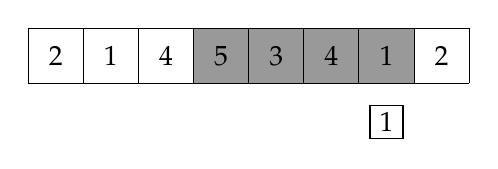
\begin{tikzpicture}[scale=0.7]
\fill[color=lightgray] (3,0) rectangle (7,1);
\draw (0,0) grid (8,1);

\node at (0.5,0.5) {$2$};
\node at (1.5,0.5) {$1$};
\node at (2.5,0.5) {$4$};
\node at (3.5,0.5) {$5$};
\node at (4.5,0.5) {$3$};
\node at (5.5,0.5) {$4$};
\node at (6.5,0.5) {$1$};
\node at (7.5,0.5) {$2$};

\draw (6.2,0.2-1.2) rectangle (6.8,0.8-1.2);

\node at (6.5,0.5-1.2) {$1$};
\end{tikzpicture}
\end{center}

Finally the window reaches its last position.
The element 2 is added to the queue,
but the smallest value inside the window
is still 1.
\begin{center}
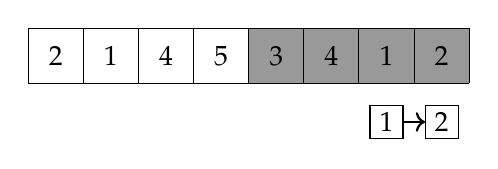
\begin{tikzpicture}[scale=0.7]
\fill[color=lightgray] (4,0) rectangle (8,1);
\draw (0,0) grid (8,1);

\node at (0.5,0.5) {$2$};
\node at (1.5,0.5) {$1$};
\node at (2.5,0.5) {$4$};
\node at (3.5,0.5) {$5$};
\node at (4.5,0.5) {$3$};
\node at (5.5,0.5) {$4$};
\node at (6.5,0.5) {$1$};
\node at (7.5,0.5) {$2$};

\draw (6.2,0.2-1.2) rectangle (6.8,0.8-1.2);
\draw (7.2,0.2-1.2) rectangle (7.8,0.8-1.2);

\node at (6.5,0.5-1.2) {$1$};
\node at (7.5,0.5-1.2) {$2$};

\draw[->,thick] (6.8,0.5-1.2) -- (7.2,0.5-1.2);
\end{tikzpicture}
\end{center}

Since each array element
is added to the queue exactly once and
removed from the queue at most once,
the algorithm works in $O(n)$ time.

\part{Dynamic Programming}
\chapter{Common DP Problems}
\section{Rod Cutting}
\begin{problem}[DP]
Given a rod of length $n$ inches and an array of prices that contains prices of all pieces of size smaller than $n$. Determine the maximum value obtainable by cutting up the rod and selling the pieces.
\end{problem}
\begin{exmp}
If length of the rod is $8$ and the values of different pieces are given as following, then the maximum obtainable value is $22$ (by cutting in two pieces of lengths $2$ and $6$).
Price  array = \texttt{[1,5,8,9,10,17,17,20]}
\end{exmp}
\begin{tcolorbox}[title=Solution]
\hfill\break
We fix the last piece of rod with length $i$ and iterate over $i$
\begin{lstlisting}
int cutRod(int price[], int n)
{
   int val[n+1]; //dp table with optimal value for rod of length 0...n
   val[0] = 0;  //base case

   for (int i = 1; i<=n; i++)
   {
       int max_val = INT_MIN;
       for (int j = 0; j < i; j++)
       {
            max_val = max(max_val, price[j] + val[i-j-1]);
       }
       val[i] = max_val; //answer for i in range 0...n
   }
   return val[n]; //answer
}
\end{lstlisting}
Time Complexity is $\mathcal{O}(n^2)$
\end{tcolorbox}
\section{Longest Increasing Subsequence(LIS)}
\begin{problem}[DP]
Find the length of the longest subsequence of a given sequence such that all elements of the subsequence are sorted in increasing order.
\end{problem}
\begin{exmp}
LIS for \texttt{[10, 22, 9, 33, 21, 50, 41, 60, 80]} is $6$ and LIS is \texttt{[10, 22, 33, 50, 60, 80]}.
\end{exmp}
\begin{tcolorbox}[title=Solution]
\hfill\break
Let \texttt{arr[0..n-1]} be the input array and \texttt{L(i)} be the length of the LIS ending at index $i$ such that \texttt{arr[i]} is the last element of the LIS.

Then, \texttt{L(i)} can be recursively written as:

\texttt{L(i) = 1 + max(L(j)) where }$0 \leq j \leq i$ and \texttt{arr[j] < arr[i];} or

\text{L(i) = 1}, if no such $j$ exists.

To find the LIS for a given array, we need to return \texttt{max(L(i))} where $0 \leq i \leq n$.
\begin{lstlisting}
int dp[n] = {0}; //dp table
for(int i =0; i<n; i++)
{
  dp[i] = 1;
  for(int k= i-1; k>=0; k--)
  {
    if(arr[k] < arr[i]) //all k such that arr[k] < arr[i]
    {
      dp[i] = max(dp[i], dp[k]+1);//include k or not
    }
  }
}
cout << dp[n-1];
\end{lstlisting}

Time Complexity is $\mathcal{O}(n^2)$
\end{tcolorbox}
\newpage
\section{Longest Common Subsequence(LCS)}
\begin{problem}
Given two sequences, find the length of longest subsequence present in both of them. A subsequence is a sequence that appears in the same relative order, but not necessarily contiguous
\end{problem}
\begin{exmp}
LCS for input Sequences \texttt{“ABCDGH”} and \texttt{“AEDFHR”} is \texttt{“ADH”} of length $3$.
\end{exmp}
\begin{exmp}
LCS for input Sequences \texttt{“AGGTAB”} and \texttt{“GXTXAYB”} is \texttt{“GTAB”} of length $4$.
\end{exmp}
\begin{tcolorbox}[title=Solution]
\hfill\break
\begin{lstlisting}
/* Returns length of LCS for X[0..m-1], Y[0..n-1] */
int lcs(string x, string y, int m, int n )
{
    int L[m+1][n+1]; //2D dp array

/* Following steps build L[m+1][n+1] in bottom up fashion. Note
that L[i][j] contains length of LCS of X[0..i-1] and Y[0..j-1] */
    for (int i=0; i<=m; i++)
    {
      for (int j=0; j<=n; j++)
      {
      if (i == 0 || j == 0) // base case
        L[i][j] = 0;

      else if (X[i-1] == Y[j-1]) //if two chars are equal
        L[i][j] = L[i-1][j-1] + 1;

      else //if two chars are not equal
        L[i][j] = max(L[i-1][j], L[i][j-1]);
      }
    }

    /* L[m][n] contains length of LCS for X[0..n-1] and Y[0..m-1] */
    return L[m][n];
}
\end{lstlisting}
Time Complexity is $\mathcal{O}(nm)$
\end{tcolorbox}
\newpage
\section{Tiling Problem}
\begin{problem}
Given a $2 \times n$ board and tiles of size $2 \times 1$, count the number of ways to tile the given board using the $2 \times 1$ tiles. A tile can either be placed horizontally i.e., as a $1 \times 2$ tile or vertically i.e., as $2 \times 1$ tile.
\end{problem}
\begin{exmp}


Input n = 3

Output: 3

Explanation:

We need 3 tiles to tile the board of size  2 x 3.

We can tile the board using following ways

1) Place all 3 tiles vertically.

2) Place first tile vertically and remaining 2 tiles horizontally.

3) Place first 2 tiles horizontally and remaining tiles vertically

The first solution is shown below
\begin{center}
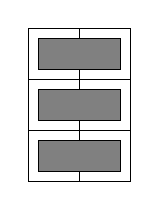
\begin{tikzpicture}[scale=.65]
    \draw (0,0) grid (2,3);
    \draw[fill=gray] (0+0.2,0+0.2) rectangle (2-0.2,1-0.2);
    \draw[fill=gray] (0+0.2,1+0.2) rectangle (2-0.2,2-0.2);
    \draw[fill=gray] (0+0.2,2+0.2) rectangle (2-0.2,3-0.2);

\end{tikzpicture}
\end{center}


\end{exmp}
\begin{exmp}


Input n = 4

Output: 5

Explanation:

For a 2 x 4 board, there are 5 ways

1) All 4 vertical

2) All 4 horizontal

3) First 2 vertical, remaining 2 horizontal

4) First 2 horizontal, remaining 2 vertical

5) Corner 2 vertical, middle 2 horizontal

The third solution is shown below:

\begin{center}
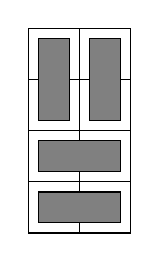
\begin{tikzpicture}[scale=.65]
    \draw (0,0) grid (2,4);
    \draw[fill=gray] (0+0.2,0+0.2) rectangle (2-0.2,1-0.2);
    \draw[fill=gray] (0+0.2,1+0.2) rectangle (2-0.2,2-0.2);
    \draw[fill=gray] (1+0.2,2+0.2) rectangle (2-0.2,4-0.2);
    \draw[fill=gray] (0+0.2,2+0.2) rectangle (1-0.2,4-0.2);

\end{tikzpicture}
\end{center}

\end{exmp}
\newpage
\begin{tcolorbox}[title=Solution]
\hfill\break
Tiling Problem is nothing but Fibonacci sequence

Method 1:


\begin{lstlisting}
int fib(int n)
{
    //Space optimized Fibonacci
    int a = 1, b = 1, c, i;
    if( n == 1 || n==2)
      return n;
    for (i = 2; i <= n; i++)
    {
      c = a + b;
      a = b;
      b = c;
    }
    return b;
}
\end{lstlisting}

Time Complexity is $\mathcal{O}(n)$

Method 2:

In this method we directly implement the formula for $n^{th}$ term in the Fibonacci series. Time Complexity : $\mathcal{O}(1)$. Space Complexity: $\mathcal{O}(1)$
$$F_n = \frac{(\frac{(\sqrt{5} + 1)}{2})^ n}{\sqrt{5}}$$
\begin{lstlisting}
int fib(int n)
{
    double phi = (1 + sqrt(5)) / 2;
    return round(pow(phi, n) / sqrt(5));
}
\end{lstlisting}
\end{tcolorbox}
\newpage
\section{Coin - 1}
\begin{problem}
Given a value $n$, if we want to make change for $n$ cents, and we have infinite supply of each of \texttt{S = [$S_1, S_2, .. , S_m$]} valued coins, how many ways can we make the change? The order of coins does not matter.
\end{problem}
\begin{exmp}
$n = 4$ and \texttt{S = [1,2,3]} and answer = $4$

There are four solutions: \texttt{[1,1,1,1];[1,1,2];[2,2];[1,3]}
\end{exmp}
\begin{exmp}
$n = 10$ and \texttt{S = [2,5,3,6]} and answer = $5$

There are five solutions: \texttt{[2,2,2,2,2];[2,2,3,3];[2,2,6];[2,3,5];[5,5]}
\end{exmp}
\begin{tcolorbox}[title=Solution]
\hfill\break
Recursive Equation:
\begin{equation*}
    \texttt{change}(x) = \begin{cases}
               $x = 0$ & 1\\
               $x > 0$ & \sum_{c \in \texttt{coins}} \texttt{change}(x-c)\\
           \end{cases}
\end{equation*}
\begin{lstlisting}
int coin(int S[], int m, int n)
{
    // table[i] will be storing the number of solutions for
    // value i
    int table[n+1];
    // Initialize all table values as 0
    memset(table, 0, sizeof(table));
    table[0] = 1; //1 way to make 0 coins. First hand experience :)
    // Pick all coins one by one and update the table[] values
    // after the index greater than or equal to the value of the
    // picked coin
    for(int i: S) //for each coin is S
        for(int j=i; j<=n; j++)
            table[j] += table[j-i];

    return table[n]; //answer
}
\end{lstlisting}
Time Complexity is $\mathcal{O}(nm)$
\end{tcolorbox}
\newpage
\section{Coin - 2}
\begin{problem}
Given a value $n$, if we want to make change for $n$ cents, and we have infinite supply of each of \texttt{C = [ $C_1, C_2, .. , C_m$]} valued coins, what is the minimum number of coins to make the change?
\end{problem}
\begin{exmp}
\texttt{coins[] = [25, 10, 5]}, $n = 30$

Output: Minimum 2 coins required

We can use one coin of 25 cents and one of 5 cents
\end{exmp}
\begin{exmp}
\texttt{coins[] = [9, 6, 5, 1]}, $n = 11$

Output: Minimum 2 coins required

We can use one coin of 6 cents and 1 coin of 5 cents
\end{exmp}
\begin{tcolorbox}[title=Solution]
\hfill\break
\begin{lstlisting}
// m is size of coins array (number of different coins)
int minCoins(int coins[], int n)
{
    // table[i] will be storing the minimum number of coins
    // required for i value.  So table[n] will have result
    int table[n+1];

    // Base case
    table[0] = 0; //Again first hand experience :)


    // Compute minimum coins required for all
    // values from 1 to n
    for (int i=1; i<=n; i++)
    {
        table[i] = INT_MAX; //initialize all values to Infinity
        // Go through all coins smaller than i
        for (int c : coins)
        {
            if (i-c >= 0)
            {
                table[i] = min(table[i], table[i-c]+1);
            }
        }
    }
    return table[n];
}
\end{lstlisting}
Time Complexity is $\mathcal{O}(nm)$
\end{tcolorbox}
\newpage
\section{Largest Sum Contiguous Subarray}
\begin{problem}
Given an integer array $A$, find the sum of the contiguous subarray (containing at least one number) which has the largest sum. Formally, the task is to find indices $i$  and $j$  with $1\leq i\leq j\leq n$  , such that the sum
$$\sum_{x=i}^j A[x]$$ is as large as possible
\end{problem}
\begin{exmp}
Input: \texttt{[-2,1,-3,4,-1,2,1,-5,4]},

Output: $6$

Explanation: \texttt{[4,-1,2,1]} has the largest sum = 6.
\end{exmp}
\begin{tcolorbox}[title=Solution]
\hfill\break
This is called Kadane's algorithm.

The key idea of Kadane’s algorithm is to keep a running sum of the integers seen so far and
greedily reset that to $0$ if the running sum dips below $0$. This is because re-starting from
$0$ is always better than continuing from a negative running sum.

\begin{lstlisting}
int max_sum(int A[], int n)
{
    int sum = 0, ans = 0; // important, ans must be initialized to 0
    for (int i = 0; i < n; i++)
    { // linear scan, O(n)
        sum += A[i]; // we greedily extend this running sum
        ans = max(ans, sum); // we keep the maximum RSQ overall
        if (sum < 0)
        {
            sum = 0; // but we reset the running sum
        }
    } // if it ever dips below 0
    return ans; //ans is the final answer
}
\end{lstlisting}
Time Complexity is $\mathcal{O}(n)$
\end{tcolorbox}
\newpage
\section{0-1 Knapsack Part 1}
\begin{problem}
Given $n$ items, each with its own value $V_i$ and weight $W_i$, $\forall i \in [0..n-1]$, and a
maximum knapsack of size S, compute the maximum value of the items that we can carry, if
we can either ignore or take a particular item (hence the term 0-1 for ignore/take).
\end{problem}
\begin{exmp}
\hfill\break

\texttt{Value = [60,100,120]}

\texttt{Weight = [10,20,30]}

\texttt{Knapsack size = 50}

Output = $220$

Explanation: The best choice is to pick item 2 and item 3
\end{exmp}
\begin{tcolorbox}[title=Solution]
\hfill\break
\begin{lstlisting}
int knapSack(int w, int weight[], int value[], int n)
{
   int knap[n+1][w+1]; //dp table

   // Build table K[][] in bottom up manner
   for (int i = 0; i<=n; i++)
   {
       for (int j = 0; j<=w; j++)
       {
            if(i == 0 || j == 0)
            {
                knap[i][j] = 0;
            }
            else if(weight[i-1] <= j)
            {
knap[i][j] = max(value[i-1]+ knap[i-1][j-weight[i-1]], knap[i-1][j]);
            }
            else
            {
                knap[i][j] = knap[i-1][j];
            }
       }
   }

   return knap[n][w]; //answer
}
\end{lstlisting}
Time Complexity is $\mathcal{O}(nW)$ where n is the number of items and W is the capacity of knapsack.
\end{tcolorbox}
\section{0 - 1 Knapsack Part 2}
\begin{problem}
Given a list of weights $[w_1,w_2,\ldots,w_n]$, determine all sums that can be constructed using the weights
\end{problem}
\begin{exmp}
If the weights are
$[1,3,3,5]$, the following sums are possible:

\begin{center}
\begin{tabular}{rrrrrrrrrrrrr}
 0 & 1 & 2 & 3 & 4 & 5 & 6 & 7 & 8 & 9 & 10 & 11 & 12 \\
\hline
 X & X & & X & X & X & X & X & X & X & & X & X \\
\end{tabular}
\end{center}

In this case, all sums between $0 \ldots 12$
are possible, except 2 and 10.
For example, the sum 7 is possible because we
can select the weights $[1,3,3]$.
\end{exmp}
\begin{tcolorbox}[title=Solution]
\hfill\break
Let $\texttt{possible}(x,k)=\textrm{true}$ if
we can construct a sum $x$
using the first $k$ weights,
and otherwise $\texttt{possible}(x,k)=\textrm{false}$.
The recursive relation is as follows:
\[ \texttt{possible}(x,k) = \texttt{possible}(x-w_k,k-1) \lor \texttt{possible}(x,k-1) \]

The formula is based on the fact that we can
either use or not use the weight $w_k$ in the sum.
If we use $w_k$, the remaining task is to
form the sum $x-w_k$ using the first $k-1$ weights,
and if we do not use $w_k$,
the remaining task is to form the sum $x$
using the first $k-1$ weights.
The base cases are,
\begin{equation*}
    \texttt{possible}(x,0) = \begin{cases}
               \textrm{true}    & x = 0\\
               \textrm{false}   & x \neq 0 \\
           \end{cases}
\end{equation*}
\begin{lstlisting}
// Let "total" denote the total sum of the weights.
w[n]; //array of weights
possible[total+1];
possible[0] = true;
for (int k = 1; k <= n; k++)
{
    for (int x = total; x >= 0; x--)
    {
        if (possible[x]) possible[x+w[k]] = true;
    }
}
for(int i = 0; i<= total; i++)
{
    if(possible[i])
        cout << i << "\n"; //output the values which are possible
}
\end{lstlisting}
Time Complexity is $\mathcal{O}(n \times total)$
\end{tcolorbox}
\section{Maximum Sum Path in a Grid}
\begin{problem}
Find a path
from the upper-left corner to
the lower-right corner
of an $n \times n$ grid, such that
we only move down and right.
Each square contains a positive integer,
and the path should be constructed so
that the sum of the values along
the path is as large as possible.
\end{problem}
\begin{exmp}
\hfill\break
\begin{center}
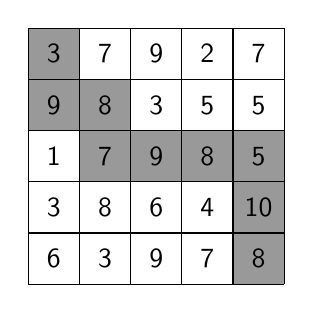
\begin{tikzpicture}[scale=.65]
  \begin{scope}
    \fill [color=lightgray] (0, 9) rectangle (1, 8);
    \fill [color=lightgray] (0, 8) rectangle (1, 7);
    \fill [color=lightgray] (1, 8) rectangle (2, 7);
    \fill [color=lightgray] (1, 7) rectangle (2, 6);
    \fill [color=lightgray] (2, 7) rectangle (3, 6);
    \fill [color=lightgray] (3, 7) rectangle (4, 6);
    \fill [color=lightgray] (4, 7) rectangle (5, 6);
    \fill [color=lightgray] (4, 6) rectangle (5, 5);
    \fill [color=lightgray] (4, 5) rectangle (5, 4);
    \draw (0, 4) grid (5, 9);
    \node at (0.5,8.5) {3};
    \node at (1.5,8.5) {7};
    \node at (2.5,8.5) {9};
    \node at (3.5,8.5) {2};
    \node at (4.5,8.5) {7};
    \node at (0.5,7.5) {9};
    \node at (1.5,7.5) {8};
    \node at (2.5,7.5) {3};
    \node at (3.5,7.5) {5};
    \node at (4.5,7.5) {5};
    \node at (0.5,6.5) {1};
    \node at (1.5,6.5) {7};
    \node at (2.5,6.5) {9};
    \node at (3.5,6.5) {8};
    \node at (4.5,6.5) {5};
    \node at (0.5,5.5) {3};
    \node at (1.5,5.5) {8};
    \node at (2.5,5.5) {6};
    \node at (3.5,5.5) {4};
    \node at (4.5,5.5) {10};
    \node at (0.5,4.5) {6};
    \node at (1.5,4.5) {3};
    \node at (2.5,4.5) {9};
    \node at (3.5,4.5) {7};
    \node at (4.5,4.5) {8};
  \end{scope}
\end{tikzpicture}
\end{center}
The sum of the values on the path is 67,
and this is the largest possible sum on a path
from the
upper-left corner to the lower-right corner.
\end{exmp}
\begin{tcolorbox}[title=Solution]
\hfill\break
The formula is based on the observation
that a path that ends at square $(y,x)$
can come either from square $(y,x-1)$
or square $(y-1,x)$:
\begin{center}
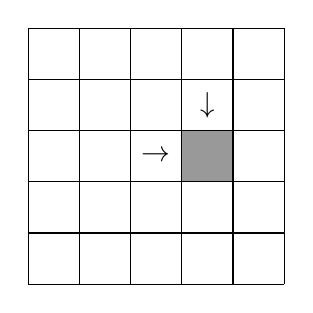
\begin{tikzpicture}[scale=.65]
  \begin{scope}
    \fill [color=lightgray] (3, 7) rectangle (4, 6);
    \draw (0, 4) grid (5, 9);

    \node at (2.5,6.5) {$\rightarrow$};
    \node at (3.5,7.5) {$\downarrow$};

  \end{scope}
\end{tikzpicture}
\end{center}
\begin{lstlisting}
value[n+1][n+1]; //grid values
int sum[n][n]; //dp array
for (int y = 1; y <= n; y++)
{
    for (int x = 1; x <= n; x++)
    {
        sum[y][x] = max(sum[y][x-1],sum[y-1][x])+value[y][x];
    }
}
\end{lstlisting}
Time Complexity is $\mathcal{O}(n^2)$
\end{tcolorbox}
\newpage
\section{Edit Distance}
\begin{problem}
Given two strings \texttt{str1} and \texttt{str2} and below operations that can performed on \texttt{str1}. Find minimum number of edits (operations) required to convert \texttt{str1} into \texttt{str2}.
\begin{itemize}
\item insert a character (e.g. \texttt{ABC} $\rightarrow$ \texttt{ABCA})
\item remove a character (e.g. \texttt{ABC} $\rightarrow$ \texttt{AC})
\item modify a character (e.g. \texttt{ABC} $\rightarrow$ \texttt{ADC})
\end{itemize}
All of the above operations are of equal cost.
\end{problem}
\begin{exmp}
Input:   str1 = "geek", str2 = "gesek"

Output:  1

We can convert str1 into str2 by inserting a 's'.
\end{exmp}
\begin{exmp}
Input:   str1 = "cat", str2 = "cut"

Output:  1

We can convert str1 into str2 by replacing 'a' with 'u'.
\end{exmp}
\begin{exmp}
The edit distance between
\texttt{LOVE} and \texttt{MOVIE} is 2,
because we can first perform the operation
 \texttt{LOVE} $\rightarrow$ \texttt{MOVE}
(modify) and then the operation
\texttt{MOVE} $\rightarrow$ \texttt{MOVIE}
(insert).
The following table shows the values of \texttt{distance}
in the example case:
\begin{center}
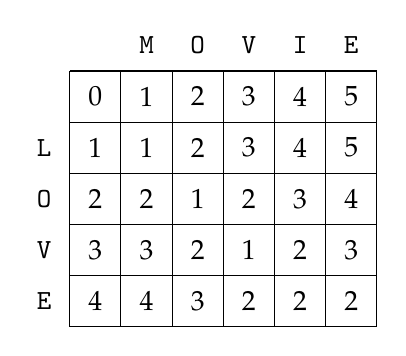
\begin{tikzpicture}[scale=.65]
  \begin{scope}
    %\fill [color=lightgray] (5, -3) rectangle (6, -4);
    \draw (1, -1) grid (7, -6);

    \node at (0.5,-2.5) {\texttt{L}};
    \node at (0.5,-3.5) {\texttt{O}};
    \node at (0.5,-4.5) {\texttt{V}};
    \node at (0.5,-5.5) {\texttt{E}};

    \node at (2.5,-0.5) {\texttt{M}};
    \node at (3.5,-0.5) {\texttt{O}};
    \node at (4.5,-0.5) {\texttt{V}};
    \node at (5.5,-0.5) {\texttt{I}};
    \node at (6.5,-0.5) {\texttt{E}};

    \node at (1.5,-1.5) {$0$};
    \node at (1.5,-2.5) {$1$};
    \node at (1.5,-3.5) {$2$};
    \node at (1.5,-4.5) {$3$};
    \node at (1.5,-5.5) {$4$};
    \node at (2.5,-1.5) {$1$};
    \node at (2.5,-2.5) {$1$};
    \node at (2.5,-3.5) {$2$};
    \node at (2.5,-4.5) {$3$};
    \node at (2.5,-5.5) {$4$};
    \node at (3.5,-1.5) {$2$};
    \node at (3.5,-2.5) {$2$};
    \node at (3.5,-3.5) {$1$};
    \node at (3.5,-4.5) {$2$};
    \node at (3.5,-5.5) {$3$};
    \node at (4.5,-1.5) {$3$};
    \node at (4.5,-2.5) {$3$};
    \node at (4.5,-3.5) {$2$};
    \node at (4.5,-4.5) {$1$};
    \node at (4.5,-5.5) {$2$};
    \node at (5.5,-1.5) {$4$};
    \node at (5.5,-2.5) {$4$};
    \node at (5.5,-3.5) {$3$};
    \node at (5.5,-4.5) {$2$};
    \node at (5.5,-5.5) {$2$};
    \node at (6.5,-1.5) {$5$};
    \node at (6.5,-2.5) {$5$};
    \node at (6.5,-3.5) {$4$};
    \node at (6.5,-4.5) {$3$};
    \node at (6.5,-5.5) {$2$};
  \end{scope}
\end{tikzpicture}
\end{center}

The lower-right corner of the table
tells us that the edit distance between
\texttt{LOVE} and \texttt{MOVIE} is 2.
The table also shows how to construct
the shortest sequence of editing operations.
In this case the path is as follows:

\begin{center}
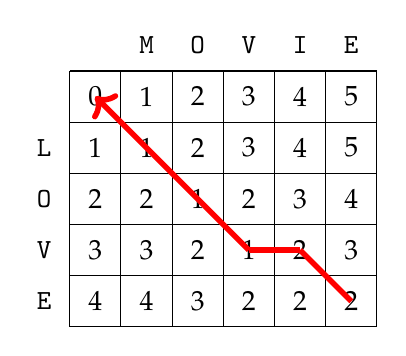
\begin{tikzpicture}[scale=.65]
  \begin{scope}
    \draw (1, -1) grid (7, -6);

    \node at (0.5,-2.5) {\texttt{L}};
    \node at (0.5,-3.5) {\texttt{O}};
    \node at (0.5,-4.5) {\texttt{V}};
    \node at (0.5,-5.5) {\texttt{E}};

    \node at (2.5,-0.5) {\texttt{M}};
    \node at (3.5,-0.5) {\texttt{O}};
    \node at (4.5,-0.5) {\texttt{V}};
    \node at (5.5,-0.5) {\texttt{I}};
    \node at (6.5,-0.5) {\texttt{E}};

    \node at (1.5,-1.5) {$0$};
    \node at (1.5,-2.5) {$1$};
    \node at (1.5,-3.5) {$2$};
    \node at (1.5,-4.5) {$3$};
    \node at (1.5,-5.5) {$4$};
    \node at (2.5,-1.5) {$1$};
    \node at (2.5,-2.5) {$1$};
    \node at (2.5,-3.5) {$2$};
    \node at (2.5,-4.5) {$3$};
    \node at (2.5,-5.5) {$4$};
    \node at (3.5,-1.5) {$2$};
    \node at (3.5,-2.5) {$2$};
    \node at (3.5,-3.5) {$1$};
    \node at (3.5,-4.5) {$2$};
    \node at (3.5,-5.5) {$3$};
    \node at (4.5,-1.5) {$3$};
    \node at (4.5,-2.5) {$3$};
    \node at (4.5,-3.5) {$2$};
    \node at (4.5,-4.5) {$1$};
    \node at (4.5,-5.5) {$2$};
    \node at (5.5,-1.5) {$4$};
    \node at (5.5,-2.5) {$4$};
    \node at (5.5,-3.5) {$3$};
    \node at (5.5,-4.5) {$2$};
    \node at (5.5,-5.5) {$2$};
    \node at (6.5,-1.5) {$5$};
    \node at (6.5,-2.5) {$5$};
    \node at (6.5,-3.5) {$4$};
    \node at (6.5,-4.5) {$3$};
    \node at (6.5,-5.5) {$2$};

    \path[draw=red,thick,-,line width=2pt] (6.5,-5.5) -- (5.5,-4.5);
    \path[draw=red,thick,-,line width=2pt] (5.5,-4.5) -- (4.5,-4.5);
    \path[draw=red,thick,->,line width=2pt] (4.5,-4.5) -- (1.5,-1.5);
  \end{scope}
\end{tikzpicture}
\end{center}
\end{exmp}
\newpage
\begin{tcolorbox}[title=Solution]
\hfill\break
\begin{lstlisting}
int editDistDP(string str1, string str2, int m, int n)
{
    // Create a table to store results of subproblems
    int dp[m+1][n+1];

    // Fill d[][] in bottom up manner
    for (int i=0; i<=m; i++)
    {
        for (int j=0; j<=n; j++)
        {
            // If first string is empty, only option is to
            // insert all characters of second string
            if (i==0)
                dp[i][j] = j;  // Min. operations = j

            // If second string is empty, only option is to
            // remove all characters of second string
            else if (j==0)
                dp[i][j] = i; // Min. operations = i

            // If last characters are same, ignore last char
            // and recur for remaining string
            else if (str1[i-1] == str2[j-1])
                dp[i][j] = dp[i-1][j-1];

            // If the last character is different, consider all
            // possibilities and find the minimum
            else
                dp[i][j] = 1 + min(dp[i][j-1],  // Insert
                                   dp[i-1][j],  // Remove
                                   dp[i-1][j-1]); // Replace
        }
    }

    return dp[m][n];
}
\end{lstlisting}
Time Complexity is $\mathcal{O}(mn)$
\end{tcolorbox}
\newpage
\section{Express \texorpdfstring{$n$}{n} as sum of \texorpdfstring{$k$}{k} numbers}
\begin{problem}
Given an integer $n$, how many ways can $K$ non-negative
integers less than or equal to $n$ add up to $n$?
\end{problem}
\begin{exmp}
$N = 5$, $K = 3$

Output: 6

The possible combinations of integers are:

( 1, 1, 3 )

( 1, 3, 1 )

( 3, 1, 1 )

( 1, 2, 2 )

( 2, 2, 1 )

( 2, 1, 2 )
\end{exmp}
\begin{exmp}
$N = 10$, $K = 4$

Output: 84
\end{exmp}
\begin{tcolorbox}[title=Solution]
\hfill\break
This is also called as the Binomial Coefficient Problem
\begin{lstlisting}
// Returns value of Binomial Coefficient C(n, k)
int binomial(int n, int k)
{
    int C[n + 1][k + 1];

    // Calculate value of Binomial Coefficient in bottom up manner
    for (int i = 0; i <= n; i++) {
        for (int j = 0; j <= min(i, k); j++) {
            // Base Cases
            if (j == 0 || j == i)
                C[i][j] = 1;

            // Calculate value using previously stored values
            else
                C[i][j] = C[i - 1][j - 1] + C[i - 1][j];
        }
    }

    return C[n][k];
}
\end{lstlisting}
Time Complexity is $\mathcal{O}(nk)$
\end{tcolorbox}
\part{Basic Graph Theory}
\chapter{Graph Theory}
\section{Formal Definition of Graph}
\key{Graph} is an abstract mathematical structure, to model pairwise relations between discrete objects. A graph $G = (V,E)$ consists of a finite set $V$ ( set of vertices or \key{nodes} ) and a set $E$ (set of \key{edges} ) of 2-subsets of $V$. Each edge is a relation ( adjacency ) between two vertices. In general, the number of vertices is denoted by $n$ and the number of edges is denoted by $m$. The following graph has 6 nodes and 9 edges.

\begin{center}
  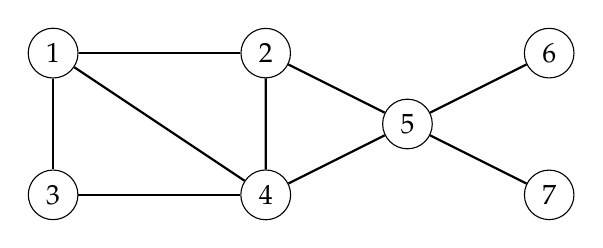
\begin{tikzpicture}[scale=0.9]
  \node[draw, circle] (1) at (1,3) {$1$};
  \node[draw, circle] (2) at (4,3) {$2$};
  \node[draw, circle] (3) at (1,1) {$3$};
  \node[draw, circle] (4) at (4,1) {$4$};
  \node[draw, circle] (5) at (6,2) {$5$};
  \node[draw, circle] (6) at (8,3) {$6$};
  \node[draw, circle] (7) at (8,1) {$7$};

  \path[draw,thick,-] (1) -- (2);
  \path[draw,thick,-] (1) -- (3);
  \path[draw,thick,-] (1) -- (4);
  \path[draw,thick,-] (3) -- (4);
  \path[draw,thick,-] (2) -- (4);
  \path[draw,thick,-] (2) -- (5);
  \path[draw,thick,-] (4) -- (5);
  \path[draw,thick,-] (5) -- (6);
  \path[draw,thick,-] (5) -- (7);
  \end{tikzpicture}
\end{center}
\section{Degree of Node}
The degree of a node $v$ is the number of edges which are joint to $v$ i.e., the number of edges that are incident on $v$. As each edge contributes 2 to the degree of its endpoints, the sum of all degrees of vertices equals twice the number of edges. The degree of node 2 in the below graph is 3.

\begin{center}
  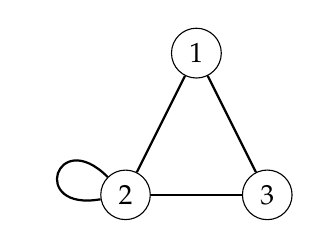
\begin{tikzpicture}[scale=0.9]
  \node[draw, circle] (1) at (2,3) {$1$};
  \node[draw, circle] (2) at (1,1) {$2$};
  \node[draw, circle] (3) at (3,1) {$3$};

  \path[draw,thick,-] (1) -- (2);
  \path[draw,thick,-] (3) -- (2);
  \path[draw,thick,-] (1) -- (3);
  \tikzset{every loop/.style={in=135,out=190}}
  \path[draw,thick,-] (2) edge [loop left] (2);
  \end{tikzpicture}
\end{center}

Note: A loop contributes 2 to the degree of the vertex it is incident on.
\section{Path}

A \key{path} leads from node $a$ to node $b$
through edges of the graph.
The \key{length} of a path is the number of
edges in it.
For example, the above graph contains
a path $1 \rightarrow 3 \rightarrow 4 \rightarrow 5$
of length 3
from node 1 to node 5:

\begin{center}
  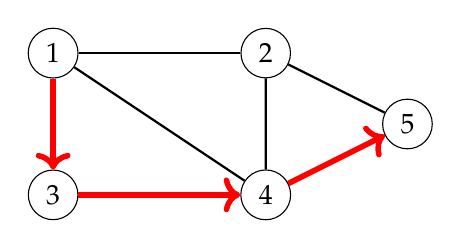
\begin{tikzpicture}[scale=0.9]
  \node[draw, circle] (1) at (1,3) {$1$};
  \node[draw, circle] (2) at (4,3) {$2$};
  \node[draw, circle] (3) at (1,1) {$3$};
  \node[draw, circle] (4) at (4,1) {$4$};
  \node[draw, circle] (5) at (6,2) {$5$};

  \path[draw,thick,-] (1) -- (2);
  \path[draw,thick,-] (1) -- (3);
  \path[draw,thick,-] (1) -- (4);
  \path[draw,thick,-] (3) -- (4);
  \path[draw,thick,-] (2) -- (4);
  \path[draw,thick,-] (2) -- (5);
  \path[draw,thick,-] (4) -- (5);

  \path[draw=red,thick,->,line width=2pt] (1) -- (3);
  \path[draw=red,thick,->,line width=2pt] (3) -- (4);
  \path[draw=red,thick,->,line width=2pt] (4) -- (5);
  \end{tikzpicture}
\end{center}

A path is a \key{cycle} if the first and last
node is the same.
For example, the above graph contains
a cycle $1 \rightarrow 3 \rightarrow 4 \rightarrow 1$.
A path is \key{simple} if each node appears
at most once in the path.

\section{Connectivity}


A graph is connected when there is a path(not necessarily a direct edge) between every pair of vertices. In a connected graph, there are no unreachable vertices. A graph that is not connected is disconnected.
For example, the following graph is connected:
\begin{center}
  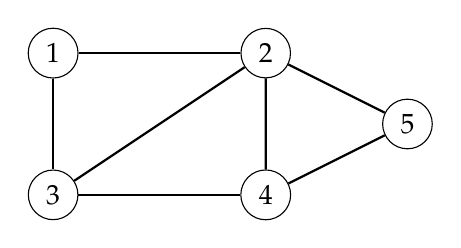
\begin{tikzpicture}[scale=0.9]
  \node[draw, circle] (1) at (1,3) {$1$};
  \node[draw, circle] (2) at (4,3) {$2$};
  \node[draw, circle] (3) at (1,1) {$3$};
  \node[draw, circle] (4) at (4,1) {$4$};
  \node[draw, circle] (5) at (6,2) {$5$};

  \path[draw,thick,-] (1) -- (2);
  \path[draw,thick,-] (1) -- (3);
  \path[draw,thick,-] (2) -- (3);
  \path[draw,thick,-] (3) -- (4);
  \path[draw,thick,-] (2) -- (4);
  \path[draw,thick,-] (2) -- (5);
  \path[draw,thick,-] (4) -- (5);
  \end{tikzpicture}
\end{center}

The following graph is not connected,
because it is not possible to get
from node 5 to any other node and vice-versa:
\begin{center}
  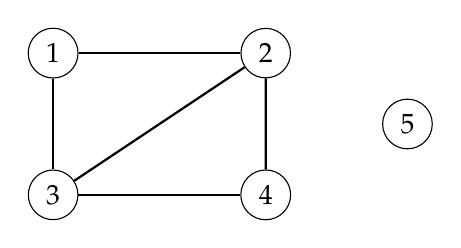
\begin{tikzpicture}[scale=0.9]
  \node[draw, circle] (1) at (1,3) {$1$};
  \node[draw, circle] (2) at (4,3) {$2$};
  \node[draw, circle] (3) at (1,1) {$3$};
  \node[draw, circle] (4) at (4,1) {$4$};
  \node[draw, circle] (5) at (6,2) {$5$};

  \path[draw,thick,-] (1) -- (2);
  \path[draw,thick,-] (1) -- (3);
  \path[draw,thick,-] (2) -- (3);
  \path[draw,thick,-] (3) -- (4);
  \path[draw,thick,-] (2) -- (4);
  \end{tikzpicture}
\end{center}


The connected parts of a graph are
called its \key{components}.
For example, the following graph
contains three components:
$\{1,\,2,\,3\}$ and $\{4,\,5,\,6,\,7\}$
\begin{center}
  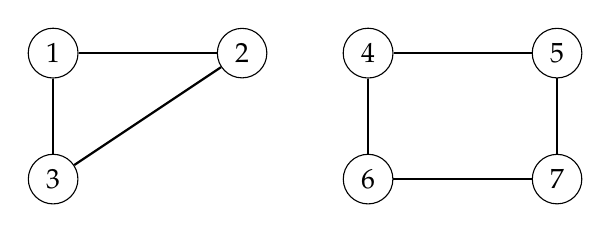
\begin{tikzpicture}[scale=0.8]
  \node[draw, circle] (1) at (1,3) {$1$};
  \node[draw, circle] (2) at (4,3) {$2$};
  \node[draw, circle] (3) at (1,1) {$3$};

  \node[draw, circle] (6) at (6,1) {$6$};
  \node[draw, circle] (7) at (9,1) {$7$};
  \node[draw, circle] (4) at (6,3) {$4$};
  \node[draw, circle] (5) at (9,3) {$5$};

  \path[draw,thick,-] (1) -- (2);
  \path[draw,thick,-] (2) -- (3);
  \path[draw,thick,-] (1) -- (3);
  \path[draw,thick,-] (4) -- (5);
  \path[draw,thick,-] (5) -- (7);
  \path[draw,thick,-] (6) -- (7);
  \path[draw,thick,-] (6) -- (4);
  \end{tikzpicture}
\end{center}

\section{Trees}
A tree is an undirected graph in which any two vertices are connected by exactly one path. It consists of $n$ nodes and $n-1$ edges. A tree cannot contain any cycles or self loops, however, the same does not apply to graphs.
For example, the following graph is a tree:

\begin{center}
  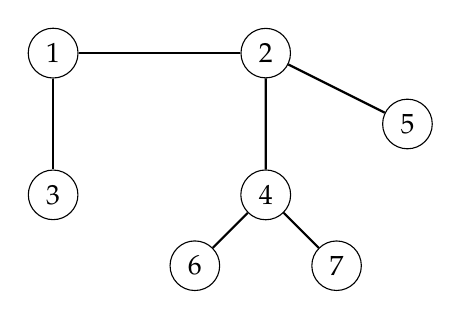
\begin{tikzpicture}[scale=0.9]
  \node[draw, circle] (1) at (1,3) {$1$};
  \node[draw, circle] (2) at (4,3) {$2$};
  \node[draw, circle] (3) at (1,1) {$3$};
  \node[draw, circle] (4) at (4,1) {$4$};
  \node[draw, circle] (5) at (6,2) {$5$};
  \node[draw, circle] (6) at (3,0) {$6$};
  \node[draw, circle] (7) at (5,0) {$7$};

  \path[draw,thick,-] (1) -- (2);
  \path[draw,thick,-] (1) -- (3);
  \path[draw,thick,-] (2) -- (5);
  \path[draw,thick,-] (2) -- (4);
  \path[draw,thick,-] (4) -- (6);
  \path[draw,thick,-] (4) -- (7);
  \end{tikzpicture}
\end{center}

A binary tree is a tree in which each node has at most two children, which are referred to as the left child and the right child. The following tree is a binary tree of size 13 and depth 3, with 1 at the root:

\begin{center}
  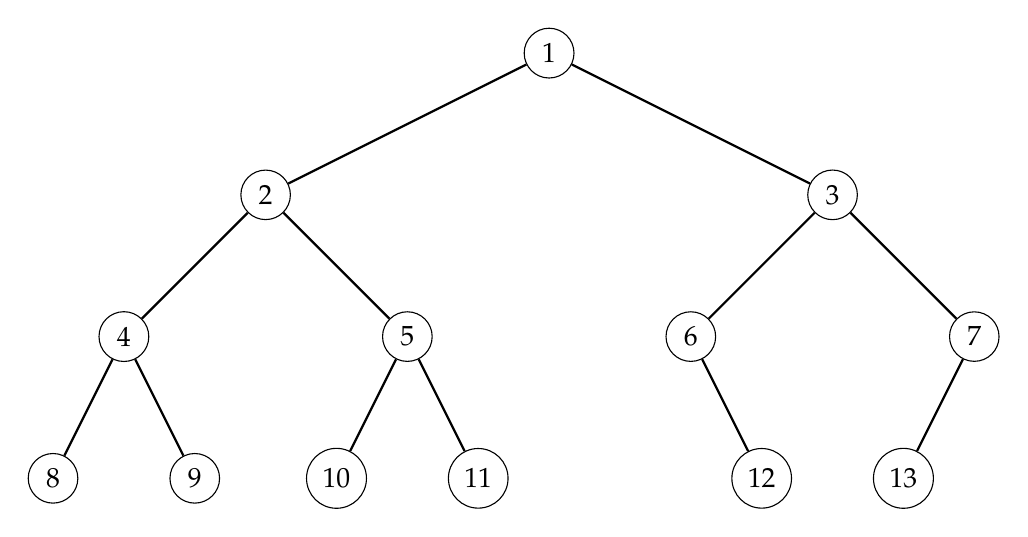
\begin{tikzpicture}[scale=0.9]
  \node[draw, circle] (1) at (8,6) {$1$};
  \node[draw, circle] (2) at (4,4) {$2$};
  \node[draw, circle] (3) at (12,4) {$3$};
  \node[draw, circle] (4) at (2,2) {$4$};
  \node[draw, circle] (5) at (6,2) {$5$};
  \node[draw, circle] (6) at (10,2) {$6$};
  \node[draw, circle] (7) at (14,2) {$7$};
  \node[draw, circle] (8) at (1,0) {$8$};
  \node[draw, circle] (9) at (3,0) {$9$};
  \node[draw, circle] (10) at (5,0) {$10$};
  \node[draw, circle] (11) at (7,0) {$11$};
  \node[draw, circle] (12) at (11,0) {$12$};
  \node[draw, circle] (13) at (13,0) {$13$};

  \path[draw,thick,-] (1) -- (2);
  \path[draw,thick,-] (1) -- (3);
  \path[draw,thick,-] (2) -- (5);
  \path[draw,thick,-] (2) -- (4);
  \path[draw,thick,-] (4) -- (8);
  \path[draw,thick,-] (4) -- (9);
  \path[draw,thick,-] (5) -- (10);
  \path[draw,thick,-] (5) -- (11);
  \path[draw,thick,-] (3) -- (6);
  \path[draw,thick,-] (3) -- (7);
  \path[draw,thick,-] (6) -- (12);
  \path[draw,thick,-] (7) -- (13);
  \end{tikzpicture}
\end{center}

\section{Types of Graphs}
\subsection{Undirected Graph}

An undirected graph is a graph in which all the edges are bi-directional i.e. the edges do not point in any specific direction. The following graph is undirected:

\begin{center}
  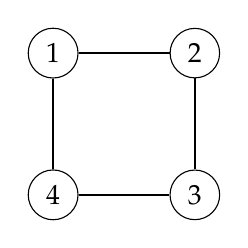
\begin{tikzpicture}[scale=0.9]
  \node[draw, circle] (1) at (1,3) {$1$};
  \node[draw, circle] (2) at (3,3) {$2$};
  \node[draw, circle] (3) at (3,1) {$3$};
  \node[draw, circle] (4) at (1,1) {$4$};

  \path[draw,thick,-] (1) -- (2);
  \path[draw,thick,-] (2) -- (3);
  \path[draw,thick,-] (3) -- (4);
  \path[draw,thick,-] (4) -- (1);
  \end{tikzpicture}
\end{center}

\subsection{Directed Graph}

A directed graph is a graph in which all the edges are uni-directional i.e. the edges point in a single direction. A typical example would be an airways map. The following graph is directed:

\begin{center}
  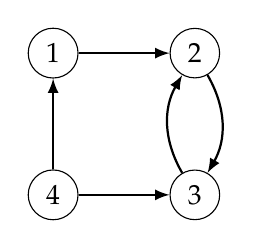
\begin{tikzpicture}[scale=0.9]
  \node[draw, circle] (1) at (1,3) {$1$};
  \node[draw, circle] (2) at (3,3) {$2$};
  \node[draw, circle] (3) at (3,1) {$3$};
  \node[draw, circle] (4) at (1,1) {$4$};

  \path[draw,thick,->,>=latex] (1) -- (2);
  \path[draw,thick,->,>=latex] (3) edge [bend left=30] (2);
  \path[draw,thick,->,>=latex] (4) -- (1);
  \path[draw,thick,->,>=latex] (4) -- (3);
  \path[draw,thick,->,>=latex] (2) edge [bend left=30] (3);
  \end{tikzpicture}
\end{center}

\subsection{Weighted Graph}

In a weighted graph, each edge is assigned a weight or cost. Consider a graph of 4 nodes as in the diagram below. As you can see each edge has a weight/cost assigned to it. Many problems are based on how to minimize/maximize the cost of a path. In the following graph, if you want to go from vertex 1 to vertex 3, you can take one of the following 3 paths:

\begin{enumerate}
    \item $1 \rightarrow 2 \rightarrow 3$ \key{Cost = 3}
    \item $1 \rightarrow 3$ \key{Cost = 1}
    \item $1 \rightarrow 4 \rightarrow 3$ \key{Cost = 5}
\end{enumerate}

\begin{center}
  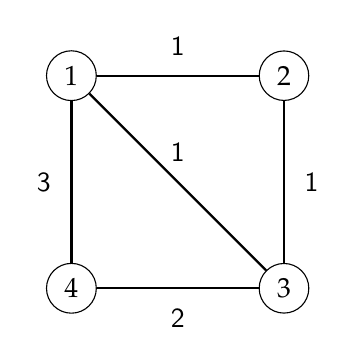
\begin{tikzpicture}[scale=0.9]
  \node[draw, circle] (1) at (1,4) {$1$};
  \node[draw, circle] (2) at (4,4) {$2$};
  \node[draw, circle] (3) at (4,1) {$3$};
  \node[draw, circle] (4) at (1,1) {$4$};

  \path[draw,thick,-] (1) -- node[font=\small,label=above:1] {} (2);
  \path[draw,thick,-] (2) -- node[font=\small,label=right:1] {} (3);
  \path[draw,thick,-] (3) -- node[font=\small,label=below:2] {} (4);
  \path[draw,thick,-] (4) -- node[font=\small,label=left:3] {} (1);
  \path[draw,thick,-] (1) -- node[font=\small,label=above:1] {} (3);
  \end{tikzpicture}
\end{center}

\subsection{Cyclic Graph}

A graph is cyclic if the graph comprises a cycle(a path that starts from a vertex and ends at the same vertex). An acyclic graph is a graph that has no cycle. The following is a cyclic directed graph.

\begin{center}
  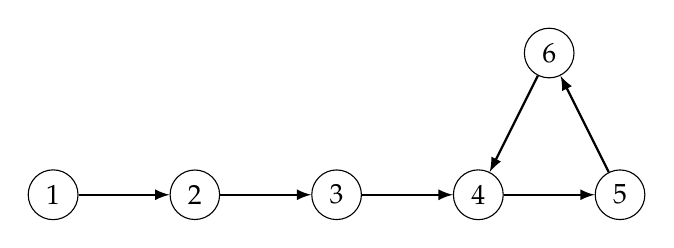
\begin{tikzpicture}[scale=0.9]
  \node[draw, circle] (1) at (1,3) {$1$};
  \node[draw, circle] (2) at (3,3) {$2$};
  \node[draw, circle] (3) at (5,3) {$3$};
  \node[draw, circle] (4) at (7,3) {$4$};
  \node[draw, circle] (5) at (9,3) {$5$};
  \node[draw, circle] (6) at (8,5) {$6$};

  \path[draw,thick,->,>=latex] (1) -- (2);
  \path[draw,thick,->,>=latex] (2) -- (3);
  \path[draw,thick,->,>=latex] (3) -- (4);
  \path[draw,thick,->,>=latex] (4) -- (5);
  \path[draw,thick,->,>=latex] (5) -- (6);
  \path[draw,thick,->,>=latex] (6) -- (4);
  \end{tikzpicture}
\end{center}
\section{Graph Colouring}

In a \key{coloring} of a graph,
each node is assigned a color so that
no adjacent nodes have the same color.

A graph is \key{bipartite} if
it is possible to color it using two colors.
It turns out that a graph is bipartite
exactly when it does not contain a cycle
with an odd number of edges.
For example, the graph
\begin{center}
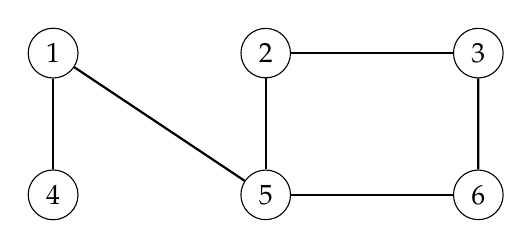
\begin{tikzpicture}[scale=0.9]
\node[draw, circle] (1) at (1,3) {$2$};
\node[draw, circle] (2) at (4,3) {$3$};
\node[draw, circle] (3) at (1,1) {$5$};
\node[draw, circle] (4) at (4,1) {$6$};
\node[draw, circle] (5) at (-2,1) {$4$};
\node[draw, circle] (6) at (-2,3) {$1$};
\path[draw,thick,-] (1) -- (2);
\path[draw,thick,-] (1) -- (3);
\path[draw,thick,-] (3) -- (4);
\path[draw,thick,-] (2) -- (4);
\path[draw,thick,-] (3) -- (6);
\path[draw,thick,-] (5) -- (6);
\end{tikzpicture}
\end{center}
is bipartite, because it can be colored as follows:
\begin{center}
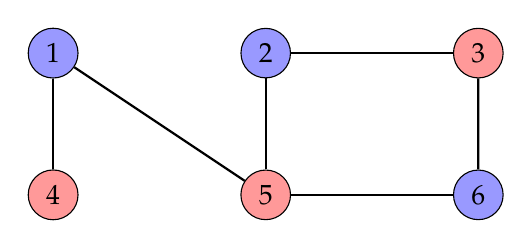
\begin{tikzpicture}[scale=0.9]
\node[draw, circle, fill=blue!40] (1) at (1,3) {$2$};
\node[draw, circle, fill=red!40] (2) at (4,3) {$3$};
\node[draw, circle, fill=red!40] (3) at (1,1) {$5$};
\node[draw, circle, fill=blue!40] (4) at (4,1) {$6$};
\node[draw, circle, fill=red!40] (5) at (-2,1) {$4$};
\node[draw, circle, fill=blue!40] (6) at (-2,3) {$1$};
\path[draw,thick,-] (1) -- (2);
\path[draw,thick,-] (1) -- (3);
\path[draw,thick,-] (3) -- (4);
\path[draw,thick,-] (2) -- (4);
\path[draw,thick,-] (3) -- (6);
\path[draw,thick,-] (5) -- (6);
\end{tikzpicture}
\end{center}
However, the graph
\begin{center}
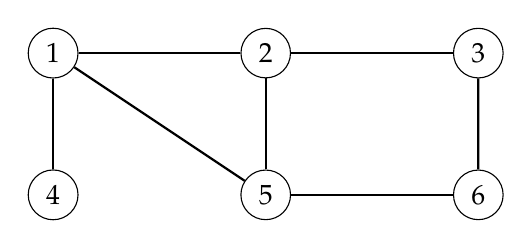
\begin{tikzpicture}[scale=0.9]
\node[draw, circle] (1) at (1,3) {$2$};
\node[draw, circle] (2) at (4,3) {$3$};
\node[draw, circle] (3) at (1,1) {$5$};
\node[draw, circle] (4) at (4,1) {$6$};
\node[draw, circle] (5) at (-2,1) {$4$};
\node[draw, circle] (6) at (-2,3) {$1$};
\path[draw,thick,-] (1) -- (2);
\path[draw,thick,-] (1) -- (3);
\path[draw,thick,-] (3) -- (4);
\path[draw,thick,-] (2) -- (4);
\path[draw,thick,-] (3) -- (6);
\path[draw,thick,-] (5) -- (6);
\path[draw,thick,-] (1) -- (6);
\end{tikzpicture}
\end{center}
is not bipartite, because it is not possible to color
the following cycle of three nodes using two colors:
\begin{center}
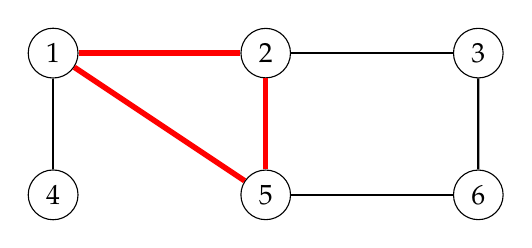
\begin{tikzpicture}[scale=0.9]
\node[draw, circle] (1) at (1,3) {$2$};
\node[draw, circle] (2) at (4,3) {$3$};
\node[draw, circle] (3) at (1,1) {$5$};
\node[draw, circle] (4) at (4,1) {$6$};
\node[draw, circle] (5) at (-2,1) {$4$};
\node[draw, circle] (6) at (-2,3) {$1$};
\path[draw,thick,-] (1) -- (2);
\path[draw,thick,-] (1) -- (3);
\path[draw,thick,-] (3) -- (4);
\path[draw,thick,-] (2) -- (4);
\path[draw,thick,-] (3) -- (6);
\path[draw,thick,-] (5) -- (6);
\path[draw,thick,-] (1) -- (6);

\path[draw=red,thick,-,line width=2pt] (1) -- (3);
\path[draw=red,thick,-,line width=2pt] (3) -- (6);
\path[draw=red,thick,-,line width=2pt] (6) -- (1);
\end{tikzpicture}
\end{center}

\subsubsection{Simplicity}


A graph is \key{simple}
if no edge starts and ends at the same node,
and there are no multiple
edges between two nodes.
Often we assume that graphs are simple.
For example, the following graph is \key{not} simple:
\begin{center}
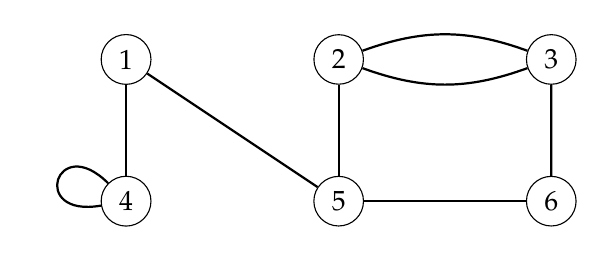
\begin{tikzpicture}[scale=0.9]
\node[draw, circle] (1) at (1,3) {$2$};
\node[draw, circle] (2) at (4,3) {$3$};
\node[draw, circle] (3) at (1,1) {$5$};
\node[draw, circle] (4) at (4,1) {$6$};
\node[draw, circle] (5) at (-2,1) {$4$};
\node[draw, circle] (6) at (-2,3) {$1$};

\path[draw,thick,-] (1) edge [bend right=20] (2);
\path[draw,thick,-] (2) edge [bend right=20] (1);
\path[draw,thick,-] (1) -- (3);
\path[draw,thick,-] (3) -- (4);
\path[draw,thick,-] (2) -- (4);
\path[draw,thick,-] (3) -- (6);
\path[draw,thick,-] (5) -- (6);

\tikzset{every loop/.style={in=135,out=190}}
\path[draw,thick,-] (5) edge [loop left] (5);
\end{tikzpicture}
\end{center}

\chapter{Graph Representation}

You can represent a graph in many ways. The choice of a data
structure depends on the size of the graph and the way the algorithm processes
it. The two most common ways of representing a graph is as follows:

\section{Adjacency matrix}

An adjacency matrix is a $n \times n$ binary matrix $A$. Element \texttt{A[i][j]} is 1 if there is an edge from vertex $i$ to vertex $j$ else is 0. In an undirected graph, if \texttt{A[i][j]} = 1, then \texttt{A[j][i]} = 1. In a directed graph, if \texttt{A[i][j]} = 1, then \texttt{A[j][i]} may or may not be 1. The matrix can be stored as an array

\begin{lstlisting}
int adj[n][n];
\end{lstlisting}

Adjacency matrix provides constant time access $\mathcal{O}(1)$ to determine if there is an edge between two nodes.But, space complexity of the adjacency matrix is $\mathcal{O}(n^2)$.

For example the graph

\begin{center}
  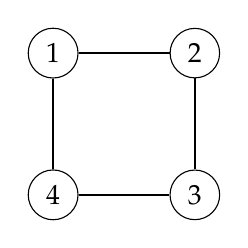
\begin{tikzpicture}[scale=0.9]
  \node[draw, circle] (1) at (1,3) {$1$};
  \node[draw, circle] (2) at (3,3) {$2$};
  \node[draw, circle] (3) at (3,1) {$3$};
  \node[draw, circle] (4) at (1,1) {$4$};

  \path[draw,thick,-] (1) -- (2);
  \path[draw,thick,-] (2) -- (3);
  \path[draw,thick,-] (3) -- (4);
  \path[draw,thick,-] (4) -- (1);
  \end{tikzpicture}
\end{center}

can be represented as follows:

\begin{center}
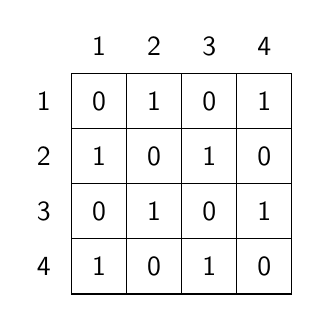
\begin{tikzpicture}[scale=0.7]
\draw (0,0) grid (4,4);
\node at (0.5,0.5) {1};
\node at (1.5,0.5) {0};
\node at (2.5,0.5) {1};
\node at (3.5,0.5) {0};
\node at (0.5,1.5) {0};
\node at (1.5,1.5) {1};
\node at (2.5,1.5) {0};
\node at (3.5,1.5) {1};
\node at (0.5,2.5) {1};
\node at (1.5,2.5) {0};
\node at (2.5,2.5) {1};
\node at (3.5,2.5) {0};
\node at (0.5,3.5) {0};
\node at (1.5,3.5) {1};
\node at (2.5,3.5) {0};
\node at (3.5,3.5) {1};
\node at (-0.5,0.5) {4};
\node at (-0.5,1.5) {3};
\node at (-0.5,2.5) {2};
\node at (-0.5,3.5) {1};
\node at (0.5,4.5) {1};
\node at (1.5,4.5) {2};
\node at (2.5,4.5) {3};
\node at (3.5,4.5) {4};
\end{tikzpicture}
\end{center}

If the graph is weighted, the adjacency matrix representation can be extended
so that the matrix contains the weight of the edge if the edge exists. Using this
representation, the graph

\begin{center}
  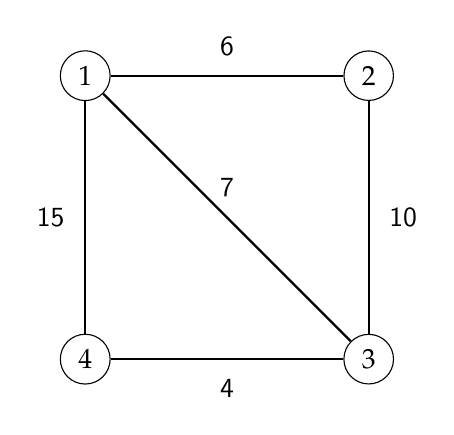
\begin{tikzpicture}[scale=0.9]
  \node[draw, circle] (1) at (1,5) {$1$};
  \node[draw, circle] (2) at (5,5) {$2$};
  \node[draw, circle] (3) at (5,1) {$3$};
  \node[draw, circle] (4) at (1,1) {$4$};

  \path[draw,thick,-] (1) -- node[font=\small,label=above:6] {} (2);
  \path[draw,thick,-] (2) -- node[font=\small,label=right:10] {} (3);
  \path[draw,thick,-] (3) -- node[font=\small,label=below:4] {} (4);
  \path[draw,thick,-] (4) -- node[font=\small,label=left:15] {} (1);
  \path[draw,thick,-] (1) -- node[font=\small,label=above:7] {} (3);
  \end{tikzpicture}
\end{center}

corresponds to the following matrix

\begin{center}
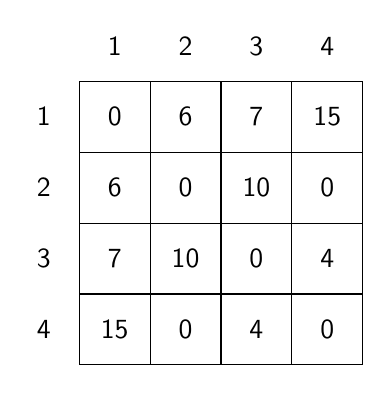
\begin{tikzpicture}[scale=0.9]
\draw (0,0) grid (4,4);
\node at (0.5,0.5) {15};
\node at (1.5,0.5) {0};
\node at (2.5,0.5) {4};
\node at (3.5,0.5) {0};
\node at (0.5,1.5) {7};
\node at (1.5,1.5) {10};
\node at (2.5,1.5) {0};
\node at (3.5,1.5) {4};
\node at (0.5,2.5) {6};
\node at (1.5,2.5) {0};
\node at (2.5,2.5) {10};
\node at (3.5,2.5) {0};
\node at (0.5,3.5) {0};
\node at (1.5,3.5) {6};
\node at (2.5,3.5) {7};
\node at (3.5,3.5) {15};
\node at (-0.5,0.5) {4};
\node at (-0.5,1.5) {3};
\node at (-0.5,2.5) {2};
\node at (-0.5,3.5) {1};
\node at (0.5,4.5) {1};
\node at (1.5,4.5) {2};
\node at (2.5,4.5) {3};
\node at (3.5,4.5) {4};
\end{tikzpicture}
\end{center}

The drawback of the adjacency matrix representation is that the matrix
contains $n^2$ elements, and usually most of them are zero. For this reason, the
representation cannot be used if the graph is large as a lot of space is wasted.

\section{Adjacency List}

The other way to represent a graph is by using an adjacency list. An adjacency list is an array $A$ of separate lists. Each element of the array $A_i$ is a list, which contains all the vertices that are adjacent to vertex $i$. In an undirected graph, if vertex $j$ is in list $A_i$ then vertex $i$ will be in list $A_j$. Adjacency List can be implemented using an array of vectors:

\begin{lstlisting}
vector<int> graph[n];
\end{lstlisting}

Then edges can be added as follows:

\begin{lstlisting}
graph[u].push_back(v);
\end{lstlisting}

For a weighted graph, the weight or cost of the edge is stored along with the vertex in the list using pairs:

\begin{lstlisting}
vector<pair<int, int>> graph[n];
\end{lstlisting}

The space complexity of adjacency list is $\mathcal{O}(V + E)$ because in an adjacency list information is stored only for those edges that actually exist in the graph. This is why adjacency list is the most popular form of representation especially in sparse graphs \footnote{A sparse matrix is a matrix in which most of the elements are zero, whereas a dense matrix is a matrix in which most of the elements are non-zero.}.

For example, the graph

\begin{center}
  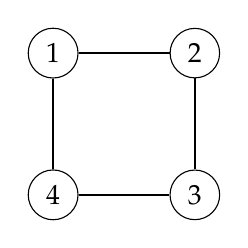
\begin{tikzpicture}[scale=0.9]
  \node[draw, circle] (1) at (1,3) {$1$};
  \node[draw, circle] (2) at (3,3) {$2$};
  \node[draw, circle] (3) at (3,1) {$3$};
  \node[draw, circle] (4) at (1,1) {$4$};

  \path[draw,thick,-] (1) -- (2);
  \path[draw,thick,-] (2) -- (3);
  \path[draw,thick,-] (3) -- (4);
  \path[draw,thick,-] (4) -- (1);
  \end{tikzpicture}
\end{center}

can be represented as:
\begin{lstlisting}
graph[1].push_back(2);
graph[1].push_back(4);
graph[2].push_back(1);
graph[2].push_back(3);
graph[3].push_back(2);
graph[3].push_back(4);
graph[4].push_back(3);
graph[4].push_back(1);
\end{lstlisting}

\begin{align*}
\resizebox{0.25\hsize}{!}{$\fbox{1}\rightarrow\fbox{2}\fbox{4}$}\\
\resizebox{0.25\hsize}{!}{$\fbox{2}\rightarrow\fbox{1}\fbox{3}$}\\
\resizebox{0.25\hsize}{!}{$\fbox{3}\rightarrow\fbox{2}\fbox{4}$} \\
\resizebox{0.25\hsize}{!}{$\fbox{4}\rightarrow\fbox{1}\fbox{3}$}
\end{align*}

Another benefit of using adjacency lists is that we can efficiently find the nodes which are directly adjacent to a given node. The following loop goes through all nodes to which we can move from node $i$ through an edge:

\begin{lstlisting}
for(auto u: graph[i])
{
    //we can reach u from i
}
\end{lstlisting}

P.S.: As a side note, it is important to take note of 0-based indexing or 1-based indexing which is used in the problem statement and adjust all graph algorithms accordingly.

\part{Graph Traversals}

\chapter{Depth First Search}
DFS is a simple graph traversal algorithm i.e. it is given a starting node in the graph, and it visits all nodes that can be reached from the starting node. The DFS algorithm is a recursive algorithm that uses the idea of backtracking. It involves exhaustive searches of all the nodes by going ahead, if possible, else by backtracking.

In simple terms, The algorithm begins at a starting node, and proceeds to all other nodes that are reachable from the starting node using the edges of the graph. All the nodes will be visited on the current path till all the unvisited nodes have been traversed after which the next path will be selected.

\section{Implementation}

This recursive nature of DFS can be implemented using recursion(duh!). The basic idea is as follows:

The following function \texttt{dfs} begins a depth-first search at a given node(usually the root node). The function assumes that the graph is stored as an adjacency list in an array

\begin{lstlisting}
vector<int> graph[n];
\end{lstlisting}

and also maintains a boolean array

\begin{lstlisting}
bool visited[n];
\end{lstlisting}

that keeps track of the visited nodes. Initially, each array value is \texttt{false}, and
when the search arrives at node $s$, the value of \texttt{visited[s]} becomes \texttt{true}. The function can be implemented as follows:
\newpage

\begin{lstlisting}
void dfs(int s) 
{
    if (visited[s]) return;
    visited[s] = true;
    // process node s
    for (auto u: adj[s]) 
    {
        dfs(u); //dfs on all nodes adjacent to s
    }
}
\end{lstlisting}

The time complexity of depth-first search is $\mathcal{O}(n+m)$
where $n$ is the number of nodes and $m$ is the
number of edges,

\section{Visualization}

DFS on a binary search tree is shown below. Note that the blue arrow reaches the root node at the end.

\begin{center}
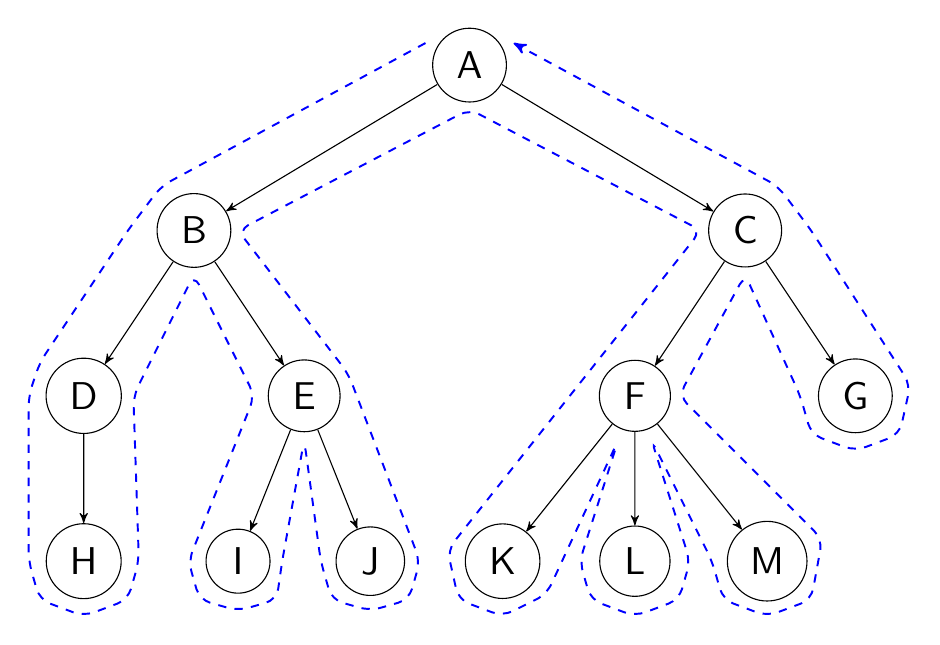
\begin{tikzpicture}[->,>=stealth',every node/.style={circle,draw},level 1/.style={sibling distance=50mm},level 2/.style={sibling distance=20mm},level 3/.style={sibling distance=12mm},
scale=1.4, transform shape
]
\node (nA){A}
   child { node (nB) {B}
              child { node (nD) {D}
                         child { node (nH) {H} }
                       }
              child {  node (nE) {E}
                         child { node (nI) {I} }
                         child { node (nJ) {J} }
                       }
            }
   child { node (nC) {C}
              child { node (nF) {F}
                         child { node (nK) {K}  }
                         child { node (nL) {L} }
                         child { node (nM) {M} }
                       }
              child {  node (nG) {G} }
             };

  \draw[->,blue,rounded corners,dashed,line width=0.7pt]
    ($(nA) + (-0.4,0.2)$) --
    ($(nB) +(-0.3,0.4)$) --
    ($(nB) +(-0.6,0.0)$) --
    ($(nD)  +(-0.4,0.3)$) --
    ($(nD)  +(-0.5,0.0)$) --
    ($(nH)  +(-0.5,0.0)$) --
    ($(nH)  +(-0.4,-0.35)$) --
    ($(nH)  +(0.0,-0.5)$) --
    ($(nH)  +(0.4,-0.35)$) --
    ($(nH)  +(0.5,0.0)$) --
%    ($(nD)  +(0.45,-0.2)$) --
    ($(nD)  +(0.45,0.0)$) --
    ($(nB)  +(0.0,-0.4)$) --
    ($(nE)  +(-0.45,0.0)$) --
    ($(nI)  +(-0.45,0.0)$) --
    ($(nI)  +(-0.35,-0.35)$) --
    ($(nI)  +(0.0,-0.45)$) --
    ($(nI)  +(0.35,-0.35)$) --
    ($(nI)  +(0.4,0.0)$) --
    ($(nE)  +(0.0,-0.4)$) --
    ($(nJ)  +(-0.45,0.0)$) --
    ($(nJ)  +(-0.35,-0.35)$) --
    ($(nJ)  +(0.0,-0.45)$) --
    ($(nJ)  +(0.35,-0.35)$) --
    ($(nJ)  +(0.45,0.0)$) --
    ($(nE)  +(0.4,0.2)$) --
    ($(nB)  +(0.4,0.0)$) --
    ($(nA)  +(0.0,-0.4)$) --
    ($(nC)  +(-0.4,0.0)$) --
%    ($(nF)  +(-0.6,0.0)$) --
    ($(nK)  +(-0.5,0.1)$) --
    ($(nK)  +(-0.4,-0.35)$) --
    ($(nK)  +(0.0,-0.5)$) --
    ($(nK)  +(0.4,-0.3)$) --
    ($(nF)  +(-0.15,-0.4)$) --
    ($(nL)  +(-0.5,0.0)$) --
    ($(nL)  +(-0.4,-0.35)$) --
    ($(nL)  +(0.0,-0.5)$) --
    ($(nL)  +(0.4,-0.35)$) --
    ($(nL)  +(0.5,0.0)$) --
    ($(nF)  +(0.15,-0.4)$) --
    ($(nM)  +(-0.5,0.0)$) --
    ($(nM)  +(-0.4,-0.35)$) --
    ($(nM)  +(0.0,-0.5)$) --
    ($(nM)  +(0.4,-0.35)$) --
    ($(nM)  +(0.5,0.2)$) --
    ($(nF)  +(0.4,0.0)$) --
    ($(nC)  +(0.0,-0.4)$) --
    ($(nG)  +(-0.5,0.0)$) --
    ($(nG)  +(-0.4,-0.35)$) --
    ($(nG)  +(0.0,-0.5)$) --
    ($(nG)  +(0.4,-0.35)$) --
    ($(nG)  +(0.5,0.1)$) --
    ($(nC) +(0.6,0.0)$) --
    ($(nC) +(0.3,0.4)$) --
    ($(nA) + (0.4,0.2)$);
\end{tikzpicture}
\end{center}

\subsection{DFS on a normal graph}

Let us consider how depth-first search processes
the following graph:

\begin{center}
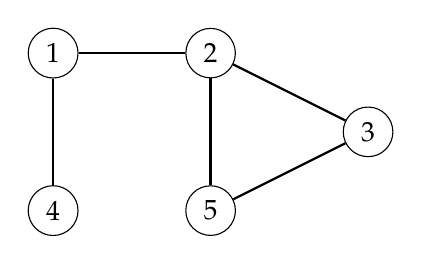
\begin{tikzpicture}
\node[draw, circle] (1) at (1,5) {$1$};
\node[draw, circle] (2) at (3,5) {$2$};
\node[draw, circle] (3) at (5,4) {$3$};
\node[draw, circle] (4) at (1,3) {$4$};
\node[draw, circle] (5) at (3,3) {$5$};

\path[draw,thick,-] (1) -- (2);
\path[draw,thick,-] (2) -- (3);
\path[draw,thick,-] (1) -- (4);
\path[draw,thick,-] (3) -- (5);
\path[draw,thick,-] (2) -- (5);
\end{tikzpicture}
\end{center}
We may begin the search at any node of the graph;
now we will begin the search at node 1.

The search first proceeds to node 2:
\begin{center}
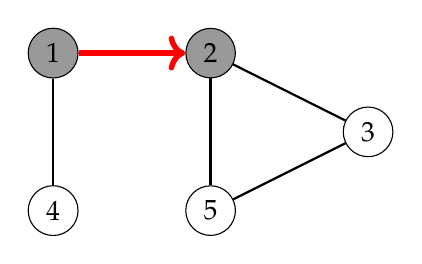
\begin{tikzpicture}
\node[draw, circle,fill=lightgray] (1) at (1,5) {$1$};
\node[draw, circle,fill=lightgray] (2) at (3,5) {$2$};
\node[draw, circle] (3) at (5,4) {$3$};
\node[draw, circle] (4) at (1,3) {$4$};
\node[draw, circle] (5) at (3,3) {$5$};

\path[draw,thick,-] (1) -- (2);
\path[draw,thick,-] (2) -- (3);
\path[draw,thick,-] (1) -- (4);
\path[draw,thick,-] (3) -- (5);
\path[draw,thick,-] (2) -- (5);

\path[draw=red,thick,->,line width=2pt] (1) -- (2);
\end{tikzpicture}
\end{center}
After this, nodes 3 and 5 will be visited:
\begin{center}
\begin{tikzpicture}
\node[draw, circle,fill=lightgray] (1) at (1,5) {$1$};
\node[draw, circle,fill=lightgray] (2) at (3,5) {$2$};
\node[draw, circle,fill=lightgray] (3) at (5,4) {$3$};
\node[draw, circle] (4) at (1,3) {$4$};
\node[draw, circle,fill=lightgray] (5) at (3,3) {$5$};

\path[draw,thick,-] (1) -- (2);
\path[draw,thick,-] (2) -- (3);
\path[draw,thick,-] (1) -- (4);
\path[draw,thick,-] (3) -- (5);
\path[draw,thick,-] (2) -- (5);

\path[draw=red,thick,->,line width=2pt] (1) -- (2);
\path[draw=red,thick,->,line width=2pt] (2) -- (3);
\path[draw=red,thick,->,line width=2pt] (3) -- (5);
\end{tikzpicture}
\end{center}
The neighbors of node 5 are 2 and 3,
but the search has already visited both of them,
so it is time to return to the previous nodes.
Also the neighbors of nodes 3 and 2
have been visited, so we next move
from node 1 to node 4:
\begin{center}
\begin{tikzpicture}
\node[draw, circle,fill=lightgray] (1) at (1,5) {$1$};
\node[draw, circle,fill=lightgray] (2) at (3,5) {$2$};
\node[draw, circle,fill=lightgray] (3) at (5,4) {$3$};
\node[draw, circle,fill=lightgray] (4) at (1,3) {$4$};
\node[draw, circle,fill=lightgray] (5) at (3,3) {$5$};

\path[draw,thick,-] (1) -- (2);
\path[draw,thick,-] (2) -- (3);
\path[draw,thick,-] (1) -- (4);
\path[draw,thick,-] (3) -- (5);
\path[draw,thick,-] (2) -- (5);

\path[draw=red,thick,->,line width=2pt] (1) -- (4);
\end{tikzpicture}
\end{center}
After this, the search terminates because it has visited
all nodes.

\section{Applications of DFS}

\subsection{Checking if Graph is Connected}

We can check if a graph is connected
by starting at an arbitrary node and
finding out if we can reach all other nodes.

For example, in the graph
\begin{center}
\begin{tikzpicture}
\node[draw, circle] (2) at (7,5) {$2$};
\node[draw, circle] (1) at (3,5) {$1$};
\node[draw, circle] (3) at (5,4) {$3$};
\node[draw, circle] (5) at (7,3) {$5$};
\node[draw, circle] (4) at (3,3) {$4$};

\path[draw,thick,-] (1) -- (3);
\path[draw,thick,-] (1) -- (4);
\path[draw,thick,-] (3) -- (4);
\path[draw,thick,-] (2) -- (5);
\end{tikzpicture}
\end{center}
a depth-first search from node $1$ visits
the following nodes:
\begin{center}
\begin{tikzpicture}
\node[draw, circle] (2) at (7,5) {$2$};
\node[draw, circle,fill=lightgray] (1) at (3,5) {$1$};
\node[draw, circle,fill=lightgray] (3) at (5,4) {$3$};
\node[draw, circle] (5) at (7,3) {$5$};
\node[draw, circle,fill=lightgray] (4) at (3,3) {$4$};

\path[draw,thick,-] (1) -- (3);
\path[draw,thick,-] (1) -- (4);
\path[draw,thick,-] (3) -- (4);
\path[draw,thick,-] (2) -- (5);

\path[draw=red,thick,->,line width=2pt] (1) -- (3);
\path[draw=red,thick,->,line width=2pt] (3) -- (4);

\end{tikzpicture}
\end{center}

Since the search did not visit all the nodes,
we can conclude that the graph is not connected.
In a similar way, we can also find all connected components
of a graph by iterating through the nodes and always
starting a new depth-first search if the current node
does not belong to any component yet.
\subsection{Detecting cycle in a graph}

\key{A Back Edge is an edge that connects a vertex to a vertex that is discovered before it's parent.}

In simple terms, A graph contains a cycle if during a graph traversal, we find a node whose neighbor(other than the previous node in the current path) has already been visited.

A graph has cycle if and only if we see a back edge during DFS. So we can run DFS for the graph and check for back edges.

\subsection{Path Finding}
We can specialize the DFS algorithm to find a path between two given vertices $u$ and $z$. The following are the steps in brief:

\begin{enumerate}
    \item Call DFS(u) with $u$ as the start vertex.
    \item Use a stack $S$ to keep track of the path between the start vertex and the current vertex.
    \item As soon as destination vertex $z$ is encountered, return the path as the i.e. the contents of the stack
\end{enumerate}

\key{This path may not be the shortest path}

\chapter{Breadth First Search}

Breadth First Search (BFS) is the most commonly used approach to traverse graph. BFS visits the nodes in increasing order of their distance
from the starting node. Thus, we can calculate the distance from the starting
node to all other nodes using breadth-first search. However, breadth-first search is more difficult to implement than depth-first search.

Breadth-first search goes through the nodes one level after another. First the
search explores the nodes whose distance from the starting node is 1, then the
nodes whose distance is 2, and so on. This process continues until all nodes have been visited.

\section{Implementation}

Breadth-first search is more difficult
to implement than depth-first search,
because the algorithm visits nodes
in different parts of the graph.
A typical implementation is based on
a queue that contains nodes.
At each step, the next node in the queue
will be processed.

The following code assumes that the graph is stored
as adjacency lists and maintains the following
data structures:
\begin{lstlisting}
queue<int> q;
bool visited[N];
int distance[N];
\end{lstlisting}

The queue \texttt{q}
contains nodes to be processed
in increasing order of their distance.
New nodes are always added to the end
of the queue, and the node at the beginning
of the queue is the next node to be processed.
The array \texttt{visited} indicates
which nodes the search has already visited,
and the array \texttt{distance} will contain the
distances from the starting node to all nodes of the graph.
\newpage
The search can be implemented as follows,
starting at node $x$:
\begin{lstlisting}
visited[x] = true;
distance[x] = 0;
q.push(x);
while (!q.empty()) {
    int s = q.front(); q.pop();
    // process node s
    for (auto u : adj[s]) {
        if (visited[u]) continue;
        visited[u] = true;
        distance[u] = distance[s]+1;
        q.push(u);
    }
}
\end{lstlisting}

Like in depth-first search,
the time complexity of breadth-first search
is $\mathcal{O}(n+m)$, where $n$ is the number of nodes
and $m$ is the number of edges.

\section{Visualization}

\begin{center}
  \begin{tikzpicture}[scale=1.2]
  \node[draw, circle] (1) at (8,6) {$1$};
  \node[draw, circle] (2) at (4,4) {$2$};
  \node[draw, circle] (3) at (12,4) {$3$};
  \node[draw, circle] (4) at (2,2) {$4$};
  \node[draw, circle] (5) at (6,2) {$5$};
  \node[draw, circle] (6) at (10,2) {$6$};
  \node[draw, circle] (7) at (14,2) {$7$};
  \node[draw, circle] (8) at (1,0) {$8$};
  \node[draw, circle] (9) at (3,0) {$9$};
  \node[draw, circle] (10) at (5,0) {$10$};
  \node[draw, circle] (11) at (7,0) {$11$};
  \node[draw, circle] (12) at (11,0) {$12$};
  \node[draw, circle] (13) at (13,0) {$13$};

  \path[draw,thick,-] (1) -- (2);
  \path[draw,thick,-] (1) -- (3);
  \path[draw,thick,-] (2) -- (5);
  \path[draw,thick,-] (2) -- (4);
  \path[draw,thick,-] (4) -- (8);
  \path[draw,thick,-] (4) -- (9);
  \path[draw,thick,-] (5) -- (10);
  \path[draw,thick,-] (5) -- (11);
  \path[draw,thick,-] (3) -- (6);
  \path[draw,thick,-] (3) -- (7);
  \path[draw,thick,-] (6) -- (12);
  \path[draw,thick,-] (7) -- (13);
  \end{tikzpicture}
\end{center}

In the above graph BFS traverses nodes in the numeric order(1-2-3-4-5-6...)
\newpage
\subsection{BFS on a normal Graph}

Let us consider how breadth-first search processes
the following graph:

\begin{center}
\begin{tikzpicture}
\node[draw, circle] (1) at (1,5) {$1$};
\node[draw, circle] (2) at (3,5) {$2$};
\node[draw, circle] (3) at (5,5) {$3$};
\node[draw, circle] (4) at (1,3) {$4$};
\node[draw, circle] (5) at (3,3) {$5$};
\node[draw, circle] (6) at (5,3) {$6$};

\path[draw,thick,-] (1) -- (2);
\path[draw,thick,-] (2) -- (3);
\path[draw,thick,-] (1) -- (4);
\path[draw,thick,-] (3) -- (6);
\path[draw,thick,-] (2) -- (5);
\path[draw,thick,-] (5) -- (6);
\end{tikzpicture}
\end{center}
Suppose that the search begins at node 1.
First, we process all nodes that can be reached
from node 1 using a single edge:
\begin{center}
\begin{tikzpicture}
\node[draw, circle,fill=lightgray] (1) at (1,5) {$1$};
\node[draw, circle,fill=lightgray] (2) at (3,5) {$2$};
\node[draw, circle] (3) at (5,5) {$3$};
\node[draw, circle,fill=lightgray] (4) at (1,3) {$4$};
\node[draw, circle] (5) at (3,3) {$5$};
\node[draw, circle] (6) at (5,3) {$6$};

\path[draw,thick,-] (1) -- (2);
\path[draw,thick,-] (2) -- (3);
\path[draw,thick,-] (1) -- (4);
\path[draw,thick,-] (3) -- (6);
\path[draw,thick,-] (2) -- (5);
\path[draw,thick,-] (5) -- (6);

\path[draw,thick,-] (1) -- (2);
\path[draw,thick,-] (2) -- (3);
\path[draw,thick,-] (1) -- (4);
\path[draw,thick,-] (2) -- (5);

\path[draw=red,thick,->,line width=2pt] (1) -- (2);
\path[draw=red,thick,->,line width=2pt] (1) -- (4);
\end{tikzpicture}
\end{center}
After this, we proceed to nodes 3 and 5:
\begin{center}
\begin{tikzpicture}
\node[draw, circle,fill=lightgray] (1) at (1,5) {$1$};
\node[draw, circle,fill=lightgray] (2) at (3,5) {$2$};
\node[draw, circle,fill=lightgray] (3) at (5,5) {$3$};
\node[draw, circle,fill=lightgray] (4) at (1,3) {$4$};
\node[draw, circle,fill=lightgray] (5) at (3,3) {$5$};
\node[draw, circle] (6) at (5,3) {$6$};

\path[draw,thick,-] (1) -- (2);
\path[draw,thick,-] (2) -- (3);
\path[draw,thick,-] (1) -- (4);
\path[draw,thick,-] (3) -- (6);
\path[draw,thick,-] (2) -- (5);
\path[draw,thick,-] (5) -- (6);

\path[draw,thick,-] (1) -- (2);
\path[draw,thick,-] (2) -- (3);
\path[draw,thick,-] (1) -- (4);
\path[draw,thick,-] (2) -- (5);

\path[draw=red,thick,->,line width=2pt] (2) -- (3);
\path[draw=red,thick,->,line width=2pt] (2) -- (5);
\end{tikzpicture}
\end{center}
Finally, we visit node 6:
\begin{center}
\begin{tikzpicture}
\node[draw, circle,fill=lightgray] (1) at (1,5) {$1$};
\node[draw, circle,fill=lightgray] (2) at (3,5) {$2$};
\node[draw, circle,fill=lightgray] (3) at (5,5) {$3$};
\node[draw, circle,fill=lightgray] (4) at (1,3) {$4$};
\node[draw, circle,fill=lightgray] (5) at (3,3) {$5$};
\node[draw, circle,fill=lightgray] (6) at (5,3) {$6$};

\path[draw,thick,-] (1) -- (2);
\path[draw,thick,-] (2) -- (3);
\path[draw,thick,-] (1) -- (4);
\path[draw,thick,-] (3) -- (6);
\path[draw,thick,-] (2) -- (5);
\path[draw,thick,-] (5) -- (6);

\path[draw,thick,-] (1) -- (2);
\path[draw,thick,-] (2) -- (3);
\path[draw,thick,-] (1) -- (4);
\path[draw,thick,-] (2) -- (5);

\path[draw=red,thick,->,line width=2pt] (3) -- (6);
\path[draw=red,thick,->,line width=2pt] (5) -- (6);
\end{tikzpicture}
\end{center}
Now we have calculated the distances
from the starting node to all nodes of the graph.
The distances are as follows:

\begin{tabular}{ll}
\\
node & distance \\
\hline
1 & 0 \\
2 & 1 \\
3 & 2 \\
4 & 1 \\
5 & 2 \\
6 & 3 \\
\\
\end{tabular}

\section{Application of BFS}

\subsection{Check whether Graph is Bipartite}

Following is a simple algorithm to find out whether a given graph is Bipartite or not using BFS.

\begin{enumerate}
    \item Assign RED color to the source vertex (putting into set U).
    \item Color all the neighbors with BLUE color (putting into set V).
    \item Color all neighbor’s neighbor with RED color (putting into set U).
    \item This way, assign color to all vertices such that it satisfies all the constraints of $m$ way coloring problem where $m = 2$.
    \item While assigning colors, if we find a neighbor which is colored with same color as current vertex, then the graph cannot be colored with 2 vertices (or graph is not Bipartite).
\end{enumerate}

\subsection{Finding Shortest path in an unweighted graph}

BFS can be used to find the shortest path in an \key{unweighted graph}. The length of shortest path can be accessed from the distance array in our implementation.

\section{0 - 1 BFS}

\begin{problem}
  Given a graph where every edge has weight as either $0$ or $k$. A source vertex is also given in the graph. Find the shortest path from source vertex to every other vertex.
\end{problem}

The basic idea is to take a path if it has edge 0 because that will unlock more paths without increasing the distance. But, using a normal queue data structure , we cannot insert and keep it sorted in $\mathcal{O}(1)$. Using priority queue cost us $\mathcal{O}(\log{n})$ to keep it sorted. The problem with the normal queue is the absence of methods which helps us to perform all of these functions :

\begin{enumerate}
    \item Remove Top Element (To get vertex for BFS)
    \item Insert At the beginning (To push a vertex with same level i.e. zero weight)
    \item Insert At the end (To push a vertex on next level i.e. one weight)
\end{enumerate}
Fortunately, all of these operations are supported by a double ended queue (or deque in C++ STL).
\newpage
\begin{lstlisting}
vector<int> d(n, INF); //distance array initialised to infinity
d[s] = 0;
deque<int> q;
q.push_front(s);
while (!q.empty()) {
    int v = q.front();
    q.pop_front();
    for (auto edge : adj[v]) {
        int u = edge.first;
        int w = edge.second;
        if (d[v] + w < d[u]) {
            d[u] = d[v] + w;
            if (w == 1)
                q.push_back(u);
            else
                q.push_front(u);
        }
    }
}
\end{lstlisting}

\part{Shortest Path Algorithms}

\chapter{Theory}

\begin{itemize}
\item Formal definition of shortest path: 

  $G = (V,E)$ weighted graph, directed or undirected. 

Weight of path $P = <v_0,v_1,v_2, \cdots, v_k>$ is $w(P) =
  \sum_{i=1}^k w(v_{i-1},v_i)$. 

Shortest path $\delta(u,v)$ from $u$ to $v$ has weight
  
  \[ \delta(u,v) = \left\{ \begin{array}{ll}
                \min\{w(P): \mbox{$P$ is path from $u$ to $v$}\} & \mbox{If
                  path exists} \\
                \infty                                     & \mbox{Otherwise} \\
              \end{array} \right. \]
            
            Example: Shortest path from $a$ to $e$ (of length 21) \\

            \centerline{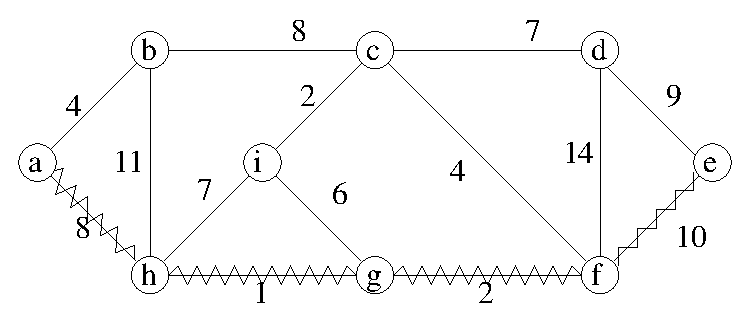
\epsfig{file=SSSP_example.eps,height=3cm}}
            
\item Properties of shortest paths:
            
\begin{itemize}
\item Subpaths of shortest paths are shortest paths: If $P = u=v_0,v_1,v_2, \cdots, v_k=v$ is shortest path from $u$ to $v$
  then for all $i$<$k$ $P' = u=v_0,v_1,v_2, \cdots, v_i$ is shortest
  path from $u$ to $v_i$
  
  
\item No (unique) shortest path exists if graph has cycle with
  negative weight \\
  
  Example: If we change weight of edge $(h,i)$ to $-8$, we have a
  cycle (i,h,g) with negative weight ($-1$). Using this we can make the 
  weight of path between $a$ and $e$ arbitrarily low by going through
  the cycle several times \\
  
  \centerline{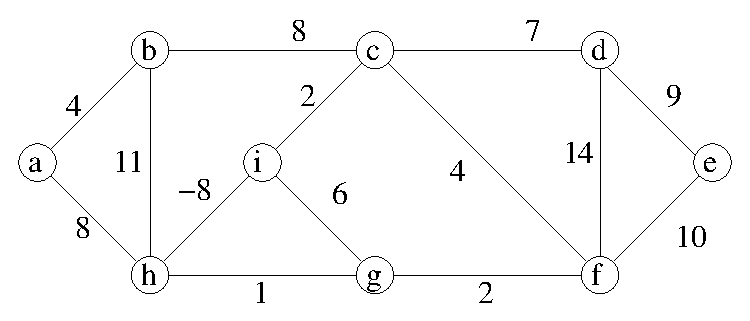
\epsfig{file=SSSP_negative.eps,height=3cm}}
  
  On the other hand, the problem is well defined if we let edge
  $(h,i)$ have weight $-7$ (no negative cycles)
\end{itemize}
\item Different variants of shortest path problem:
  \begin{itemize}
  \item {\em Single pair shortest path}: Find shortest path from $u$
    to $v$
  \item {\em Single source shortest path (SSSP)}: Find shortest path
    from source $s$ to all vertices $v \in V$
  \item {\em All pair shortest path (APSP)}: Find shortest path from
    $u$ to $v$ for all $u,v \in V$
  \end{itemize}
\item Note:
  \begin{itemize}
  \item No algorithm is known for computing a single pair shortest path
    better than solving the (``bigger'') SSSP problem
  \item APSP can be solved by running SSSP $\vert V \vert$ times \\
    $\Downarrow$ \\
    We concentrate only on the SSSP problem to solve APSP.
  \end{itemize}
\end{itemize}

\chapter{Dijkstra’s Algorithm}

Dijkstra’s algorithm for SSSP\footnote{\key{S}ingle \key{S}ource \key{S}hortest \key{P}ath : Find shortest path from source $s$ to all vertices $v \in V$} is a greedy algorithm for directed graphs\footnote{Undirected Graph is a special case of directed graph with all edges having same weight} with only \key{non-negative weights}.

Dijkstra’s algorithm maintains distances
to the nodes and reduces them during the search. Dijkstra’s algorithm is efficient,
because it only processes each edge in the graph once, using the fact that there
are no negative edges. It finds a shortest path tree from a single source node, by building a set of nodes that have minimum distance from the source

Dijkstra's algorithm can be efficiently implemented using a \texttt{priority queue} in C++ STL.

\section{Steps of Algorithm}
First we initialise three values:
\begin{enumerate}
    \item \texttt{dist[]}: an array of distances from the source node $s$ to each node in the graph, initialised the following way: \texttt{dist[s] = 0;} and for all other nodes , \texttt{dist[v]} $= \infty$. This is done at the beginning because as the algorithm proceeds, the \texttt{dist} from the source to each node $v$ in the graph will be recalculated and finalised when the shortest distance to $v$ is found.
    
    \item $Q$: a \texttt{priority queue} of all nodes in the graph. At the end of the algorithm's progress, $Q$ will be empty. $Q$ contains pairs of the form \texttt{(-d, x)}, meaning that the current distance to node $x$ is $d$. Note that the \texttt{priority queue} contains \key{negative} distances to nodes. The reason for this is that the default version of the C++ \texttt{priority queue} finds \key{maximum} elements, while we want to find \key{minimum} elements. By using negative distances, we can directly use the default \texttt{priority queue}. 
    
    \item \texttt{visited[]}: a boolean array that indicates whether a node has
    been processed. Initially all values are set to \texttt{false}.
\end{enumerate}

The steps of Dijkstra's Algorithm to find shortest distance of all vertices from vertex $s$ are as follows:
\begin{enumerate}

    \item Set all values of \texttt{dist[]} to $\infty$ except for the source vertex $s$, set \texttt{dist[s]} to $0$. Push \texttt{(0,s)} to $Q$.
    \item While $Q$ is not empty, pop the node $v$, that is not already set to \texttt{true} in \texttt{visited}, from $Q$ with the smallest \texttt{dist[v]}. In the first run, source node $s$ will be chosen because \texttt{dist[s]} was initialised to $0$. In the next run, the next node with the smallest \texttt{dist[]} value is chosen i.e. the first value in $Q$.
    \item Mark \texttt{visited[v]} as true to indicate that $v$ has been visited
    \item Update \texttt{dist[]} values of adjacent nodes of the current node $v$ as follows: for each new adjacent node $u$,
    \begin{itemize}
        \item if \texttt{dist[v]} $+$ \texttt{weight(u,v)} < \texttt{dist[u]}, there is a new minimal distance found for $u$, so update \texttt{dist[u]} to the new minimal distance value. Then push \texttt{(-dist[u],u)} to $Q$
        \item otherwise, no updates are made to \texttt{dist[u]}.
    \end{itemize}
    \item Apply the same algorithm again until $Q$ is empty.
    \item The algorithm has visited all nodes in the graph when \key{$Q$ is empty} and found the smallest distance to each node. \texttt{dist[]} now contains the shortest path tree from source $s$.
\end{enumerate}

\section{Example}

\centerline{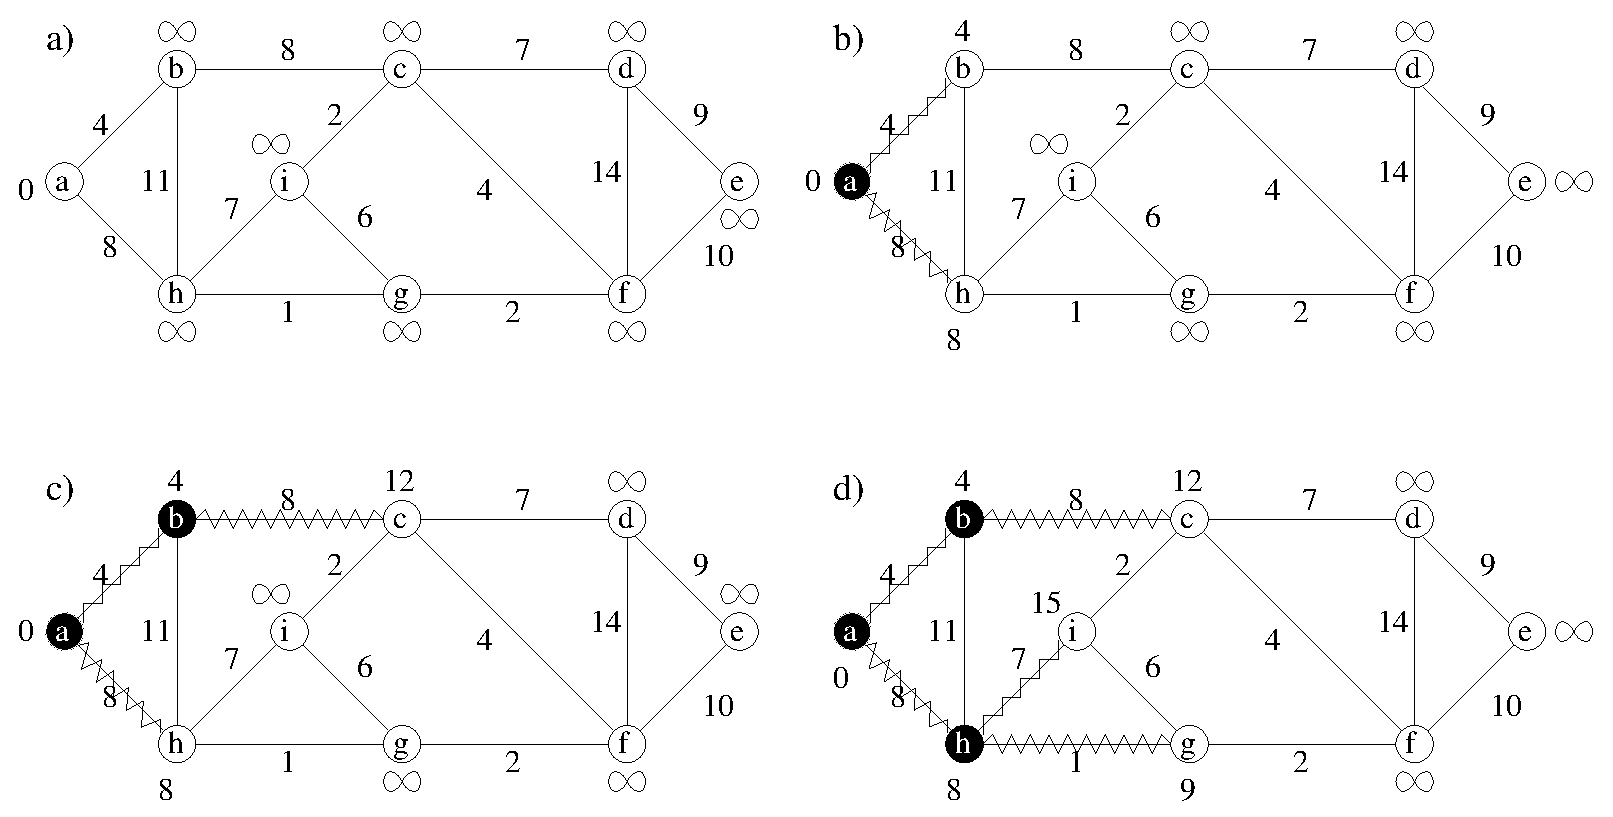
\epsfig{file=dijk_1.eps,width=13cm}}

A remarkable property in Dijkstra’s algorithm is that whenever a node is
selected, its distance is final. For example, at this point of the algorithm, the
distances 4, 8 and 12 are the final distances to nodes $b$, $h$ and $c$ respectively.

\centerline{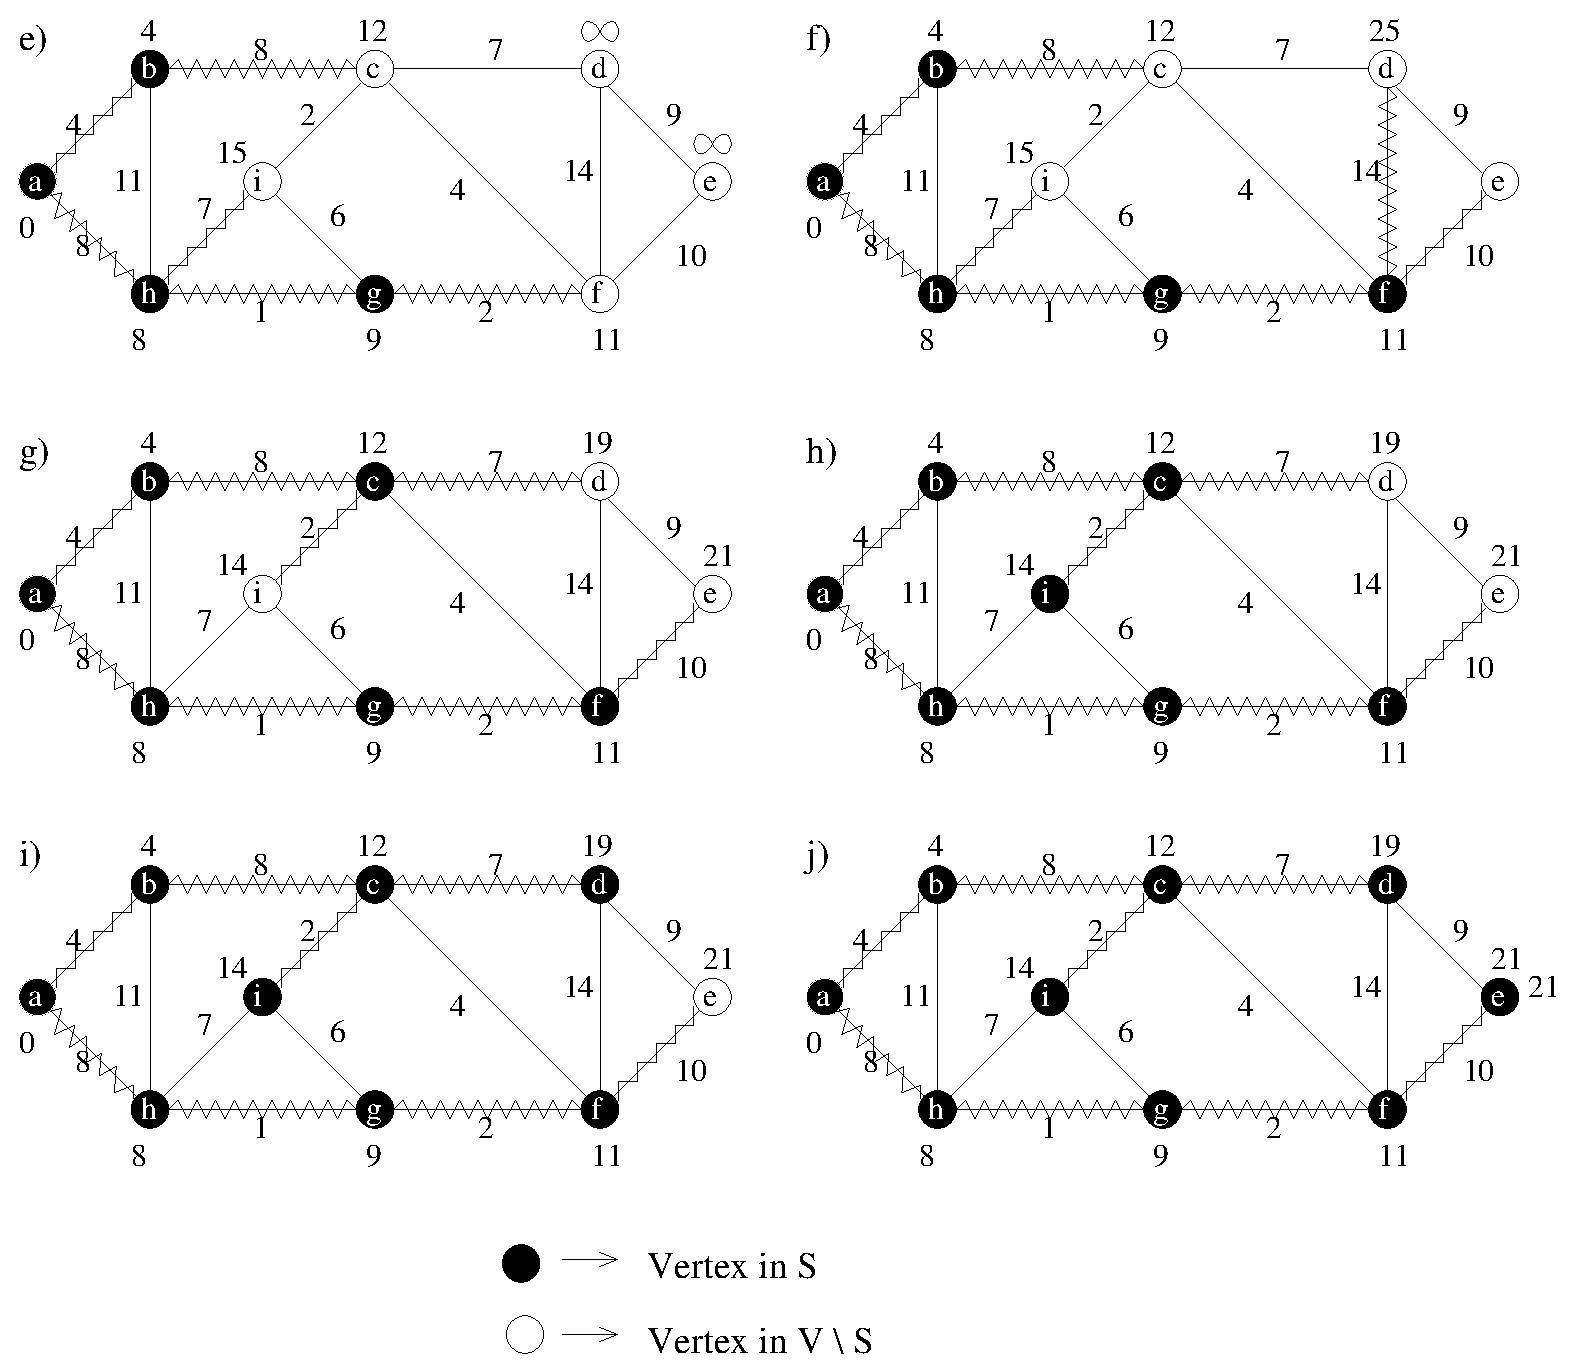
\epsfig{file=dijk_2.eps,width=13cm}}

\section{Negative Edges}

The efficiency of Dijkstra's algorithm is
based on the fact that the graph does not
contain negative edges.
If there is a negative edge,
the algorithm may give incorrect results.
As an example, consider the following graph:

\begin{center}
\begin{tikzpicture}[scale=0.9]
\node[draw, circle] (1) at (0,0) {$1$};
\node[draw, circle] (2) at (2,1) {$2$};
\node[draw, circle] (3) at (2,-1) {$3$};
\node[draw, circle] (4) at (4,0) {$4$};

\path[draw,thick,-] (1) -- node[font=\small,label=above:2] {} (2);
\path[draw,thick,-] (2) -- node[font=\small,label=above:3] {} (4);
\path[draw,thick,-] (1) -- node[font=\small,label=below:6] {} (3);
\path[draw,thick,-] (3) -- node[font=\small,label=below:$-5$] {} (4);

\path[draw=green,thick,->,line width=2pt] (1) -- (3);
\path[draw=green,thick,->,line width=2pt] (3) -- (4);
\path[draw=red,thick,->,line width=2pt] (1) -- (2);
\path[draw=red,thick,->,line width=2pt] (2) -- (4);
\end{tikzpicture}
\end{center}
\noindent
The shortest path from node 1 to node 4 is
$1 \rightarrow 3 \rightarrow 4$
and its length is 1.
However, Dijkstra's algorithm
finds the path $1 \rightarrow 2 \rightarrow 4$
by following the minimum weight edges.
The algorithm does not take into account that
on the other path, the weight $-5$
compensates the previous large weight $6$.
\newpage

\section{Implementation}

The following implementation of Dijkstra's algorithm
calculates the minimum distances from a node $x$
to other nodes of the graph.
The graph is stored as adjacency lists
so that \texttt{adj[$a$]} contains a pair $(b,w)$
always when there is an edge from node $a$ to node $b$
with weight $w$.

In the following code, the priority queue
\texttt{q} contains pairs of the form $(-d,x)$,
meaning that the current distance to node $x$ is $d$.
The array $\texttt{distance}$ contains the distance to
each node, and the array $\texttt{processed}$ indicates
whether a node has been processed.
Initially the distance is $0$ to $x$ and $\infty$ to all other nodes.

\begin{tcolorbox}[title=Solution]

\begin{lstlisting}
for (int i = 1; i <= n; i++) distance[i] = INF;
distance[x] = 0;
q.push({0,x});
while (!q.empty()) 
{
    int a = q.top().second;
    q.pop();
    if (processed[a]) continue;
    processed[a] = true;
    for (auto u : adj[a]) 
    {
        int b = u.first, w = u.second;
        if (distance[a]+w < distance[b]) 
        {
            distance[b] = distance[a]+w;
            q.push({-distance[b],b});
        }
    }
}
\end{lstlisting}

Time Complexity of this particular implementation of Dijkstra's Algorithm is $\mathcal{O}(n + m\log{m})$ because the algorithm goes through all nodes of the graph and adds for each edge at most one distance to the priority queue.


\end{tcolorbox}

\chapter{Bellman–Ford algorithm}

Bellman–Ford algorithm finds shortest paths from a starting node to all nodes of a directed graphs with \key{any weights}(but if there is a cycle with negative weight, then this problem will be \key{NP}).


\begin{tcolorbox}[title=Advantages of using Bellman-Ford over Dijkstra]
\begin{itemize}
    \setlength\itemsep{1em}
    \item Bellman-Ford supports finding shortest path in graphs with negative weight edges.
    \item Bellman-Ford can find negative weight cycles in graphs. In the $n^{th}$ step, we can reduce any distance $\iff$ we have a negative cycle.
    \item It is very easy and short to implement.
\end{itemize}
\end{tcolorbox}


But, we don't use Bellman-Ford every time because it is \key{slower} than Dijkstra.

The algorithm keeps track of distances from the starting node to all nodes
of the graph. Initially, the distance to the starting node is $0$ and the distance to
all other nodes is $\infty$. The algorithm reduces the distances by finding edges
that shorten the paths until it is not possible to reduce any distance.

\section{Pseudo-code}

\begin{algorithm}[H]
\SetAlgoLined
\KwResult{\key{S}ingle \key{S}ource \key{S}hortest \key{P}ath}
 $d[i] = \infty$ for each vertex $i$\;
 $d[v] = 0$\;
 \For{$\texttt{step} = 1$ to $n$}{
 \For{all edges $e$}{
  $i = \texttt{e.first}$ \tcp*{first end of $e$}\
  $j = \texttt{e.second}$ \tcp*{second end of $e$}\
  $w = \texttt{e.weight}$ \tcp*{weight of edge of $e$}\
  \If{$\texttt{d[j] greater than d[i]} + w$}{
    \If{$\texttt{step == n}$}
    { 
      return "Negative cycle found" \tcp*{for detecting negative cycles}\
    }
    $\texttt{d[j] = d[i]} + w$\;
   }
 }
 }
 \caption{$\texttt{Bellman-Ford(int v)}$}
\end{algorithm}

\section{Example}

Let us consider how the Bellman–Ford algorithm
works in the following graph:
\begin{center}
\begin{tikzpicture}
\node[draw, circle] (1) at (1,3) {1};
\node[draw, circle] (2) at (4,3) {2};
\node[draw, circle] (3) at (1,1) {3};
\node[draw, circle] (4) at (4,1) {4};
\node[draw, circle] (5) at (6,2) {6};
\node[color=red] at (1,3+0.55) {$0$};
\node[color=red] at (4,3+0.55) {$\infty$};
\node[color=red] at (1,1-0.55) {$\infty$};
\node[color=red] at (4,1-0.55) {$\infty$};
\node[color=red] at (6,2-0.55) {$\infty$};
\path[draw,thick,-] (1) -- node[font=\small,label=above:5] {} (2);
\path[draw,thick,-] (1) -- node[font=\small,label=left:3] {} (3);
\path[draw,thick,-] (3) -- node[font=\small,label=below:1] {} (4);
\path[draw,thick,-] (2) -- node[font=\small,label=left:3] {} (4);
\path[draw,thick,-] (2) -- node[font=\small,label=above:2] {} (5);
\path[draw,thick,-] (4) -- node[font=\small,label=below:2] {} (5);
\path[draw,thick,-] (1) -- node[font=\small,label=above:7] {} (4);
\end{tikzpicture}
\end{center}
Each node of the graph is assigned a distance.
Initially, the distance to the starting node is 0,
and the distance to all other nodes is infinite.

The algorithm searches for edges that reduce distances.
First, all edges from node 1 reduce distances:
\begin{center}
\begin{tikzpicture}
\node[draw, circle] (1) at (1,3) {1};
\node[draw, circle] (2) at (4,3) {2};
\node[draw, circle] (3) at (1,1) {3};
\node[draw, circle] (4) at (4,1) {4};
\node[draw, circle] (5) at (6,2) {5};
\node[color=red] at (1,3+0.55) {$0$};
\node[color=red] at (4,3+0.55) {$5$};
\node[color=red] at (1,1-0.55) {$3$};
\node[color=red] at (4,1-0.55) {$7$};
\node[color=red] at (6,2-0.55) {$\infty$};
\path[draw,thick,-] (1) -- node[font=\small,label=above:5] {} (2);
\path[draw,thick,-] (1) -- node[font=\small,label=left:3] {} (3);
\path[draw,thick,-] (3) -- node[font=\small,label=below:1] {} (4);
\path[draw,thick,-] (2) -- node[font=\small,label=left:3] {} (4);
\path[draw,thick,-] (2) -- node[font=\small,label=above:2] {} (5);
\path[draw,thick,-] (4) -- node[font=\small,label=below:2] {} (5);
\path[draw,thick,-] (1) -- node[font=\small,label=above:7] {} (4);

\path[draw=red,thick,->,line width=2pt] (1) -- (2);
\path[draw=red,thick,->,line width=2pt] (1) -- (3);
\path[draw=red,thick,->,line width=2pt] (1) -- (4);
\end{tikzpicture}
\end{center}
After this, edges
$2 \rightarrow 5$ and $3 \rightarrow 4$
reduce distances:
\begin{center}
\begin{tikzpicture}
\node[draw, circle] (1) at (1,3) {1};
\node[draw, circle] (2) at (4,3) {2};
\node[draw, circle] (3) at (1,1) {3};
\node[draw, circle] (4) at (4,1) {4};
\node[draw, circle] (5) at (6,2) {5};
\node[color=red] at (1,3+0.55) {$0$};
\node[color=red] at (4,3+0.55) {$5$};
\node[color=red] at (1,1-0.55) {$3$};
\node[color=red] at (4,1-0.55) {$4$};
\node[color=red] at (6,2-0.55) {$7$};
\path[draw,thick,-] (1) -- node[font=\small,label=above:5] {} (2);
\path[draw,thick,-] (1) -- node[font=\small,label=left:3] {} (3);
\path[draw,thick,-] (3) -- node[font=\small,label=below:1] {} (4);
\path[draw,thick,-] (2) -- node[font=\small,label=left:3] {} (4);
\path[draw,thick,-] (2) -- node[font=\small,label=above:2] {} (5);
\path[draw,thick,-] (4) -- node[font=\small,label=below:2] {} (5);
\path[draw,thick,-] (1) -- node[font=\small,label=above:7] {} (4);

\path[draw=red,thick,->,line width=2pt] (2) -- (5);
\path[draw=red,thick,->,line width=2pt] (3) -- (4);
\end{tikzpicture}
\end{center}
Finally, there is one more change:
\begin{center}
\begin{tikzpicture}
\node[draw, circle] (1) at (1,3) {1};
\node[draw, circle] (2) at (4,3) {2};
\node[draw, circle] (3) at (1,1) {3};
\node[draw, circle] (4) at (4,1) {4};
\node[draw, circle] (5) at (6,2) {5};
\node[color=red] at (1,3+0.55) {$0$};
\node[color=red] at (4,3+0.55) {$5$};
\node[color=red] at (1,1-0.55) {$3$};
\node[color=red] at (4,1-0.55) {$4$};
\node[color=red] at (6,2-0.55) {$6$};
\path[draw,thick,-] (1) -- node[font=\small,label=above:5] {} (2);
\path[draw,thick,-] (1) -- node[font=\small,label=left:3] {} (3);
\path[draw,thick,-] (3) -- node[font=\small,label=below:1] {} (4);
\path[draw,thick,-] (2) -- node[font=\small,label=left:3] {} (4);
\path[draw,thick,-] (2) -- node[font=\small,label=above:2] {} (5);
\path[draw,thick,-] (4) -- node[font=\small,label=below:2] {} (5);
\path[draw,thick,-] (1) -- node[font=\small,label=above:7] {} (4);

\path[draw=red,thick,->,line width=2pt] (4) -- (5);
\end{tikzpicture}
\end{center}

After this, no edge can reduce any distance.
This means that the distances are final,
and we have successfully
calculated the shortest distances
from the starting node to all nodes of the graph.

For example, the shortest distance 3
from node 1 to node 5 corresponds to
the following path:

\begin{center}
\begin{tikzpicture}
\node[draw, circle] (1) at (1,3) {1};
\node[draw, circle] (2) at (4,3) {2};
\node[draw, circle] (3) at (1,1) {3};
\node[draw, circle] (4) at (4,1) {4};
\node[draw, circle] (5) at (6,2) {5};
\node[color=red] at (1,3+0.55) {$0$};
\node[color=red] at (4,3+0.55) {$5$};
\node[color=red] at (1,1-0.55) {$3$};
\node[color=red] at (4,1-0.55) {$4$};
\node[color=red] at (6,2-0.55) {$6$};
\path[draw,thick,-] (1) -- node[font=\small,label=above:5] {} (2);
\path[draw,thick,-] (1) -- node[font=\small,label=left:3] {} (3);
\path[draw,thick,-] (3) -- node[font=\small,label=below:1] {} (4);
\path[draw,thick,-] (2) -- node[font=\small,label=left:3] {} (4);
\path[draw,thick,-] (2) -- node[font=\small,label=above:2] {} (5);
\path[draw,thick,-] (4) -- node[font=\small,label=below:2] {} (5);
\path[draw,thick,-] (1) -- node[font=\small,label=above:7] {} (4);

\path[draw=red,thick,->,line width=2pt] (1) -- (3);
\path[draw=red,thick,->,line width=2pt] (3) -- (4);
\path[draw=red,thick,->,line width=2pt] (4) -- (5);
\end{tikzpicture}
\end{center}

\section{Implementation}

The following implementation of the
Bellman–Ford algorithm determines the shortest distances
from a node $x$ to all nodes of the graph.
The code assumes that the graph is stored
as an edge list \texttt{edges}
that consists of tuples of the form $(a,b,w)$,
meaning that there is an edge from node $a$ to node $b$
with weight $w$.

The algorithm consists of $n-1$ rounds,
and on each round the algorithm goes through
all edges of the graph and tries to
reduce the distances.
The algorithm constructs an array \texttt{distance}
that will contain the distances from $x$
to all nodes of the graph.
The constant \texttt{INF} denotes an infinite distance.

\begin{tcolorbox}[title=Solution]

\begin{lstlisting}
for (int i = 1; i <= n; i++) distance[i] = INF;
distance[x] = 0;
for (int i = 1; i <= n-1; i++) {
    for (auto e : edges) {
        int a, b, w;
        tie(a, b, w) = e;
        distance[b] = min(distance[b], distance[a]+w);
    }
}
\end{lstlisting}

The time complexity of the algorithm is $\mathcal{O}(nm)$,
because the algorithm consists of $n-1$ rounds and
iterates through all $m$ edges during a round.
If there are no negative cycles in the graph,
all distances are final after $n-1$ rounds,
because each shortest path can contain at most $n-1$ edges.

\end{tcolorbox}

In practice, this algorithm can be somewhat optimised: often we already get the answer in a few phases and no useful work is done in remaining phases till $n-1$, just a waste visiting all edges. So, let's keep the flag, to tell whether something changed in the current phase or not, and if any phase, nothing changed, the algorithm can be stopped.

\begin{tcolorbox}[title=Solution]

\begin{lstlisting}
for (int i = 1; i <= n; i++) distance[i] = INF;
distance[x] = 0;
for (int i = 1; i <= n-1; i++) 
{
    bool flag = false;//flag
    for (auto e : edges) 
    {
        int a, b, w;
        tie(a, b, w) = e;
        if(distance[b] > distance[a]+w)
        {
            distance[b] = distance[a]+w;
            any = true;
        }
    }
    if(!flag)//no change takes place
    {
        break;
    }
}
\end{lstlisting}

\end{tcolorbox}
\subsection{Catching Negative Cycles}

The Bellman–Ford algorithm can also be used to
check if the graph contains a cycle with negative length.
For example, the graph

\begin{center}
\begin{tikzpicture}[scale=0.9]
\node[draw, circle] (1) at (0,0) {$1$};
\node[draw, circle] (2) at (2,1) {$2$};
\node[draw, circle] (3) at (2,-1) {$3$};
\node[draw, circle] (4) at (4,0) {$4$};

\path[draw,thick,-] (1) -- node[font=\small,label=above:$3$] {} (2);
\path[draw,thick,-] (2) -- node[font=\small,label=above:$1$] {} (4);
\path[draw,thick,-] (1) -- node[font=\small,label=below:$5$] {} (3);
\path[draw,thick,-] (3) -- node[font=\small,label=below:$-7$] {} (4);
\path[draw,thick,-] (2) -- node[font=\small,label=right:$2$] {} (3);

\path[draw=red,thick,->,line width=2pt] (2) -- (3);
\path[draw=red,thick,->,line width=2pt] (3) -- (4);
\path[draw=red,thick,->,line width=2pt] (4) -- (2);
\end{tikzpicture}
\end{center}
\noindent
contains a negative cycle
$2 \rightarrow 3 \rightarrow 4 \rightarrow 2$
with length $-4$.

If the graph contains a negative cycle,
we can shorten infinitely many times
any path that contains the cycle by repeating the cycle
again and again.
Thus, the concept of a shortest path
is not meaningful in this situation.

A negative cycle can be detected
using the Bellman–Ford algorithm by
running the algorithm for $n$ rounds.
If the last round reduces any distance,
the graph contains a negative cycle.
Note that this algorithm can be used to
search for
a negative cycle in the whole graph
regardless of the starting node.

\begin{tcolorbox}[title=Solution]

\begin{lstlisting}
for (int i = 1; i <= n; i++) distance[i] = INF;
distance[x] = 0;
for (int i = 1; i <= n-1; i++) 
{
    bool flag = false;//flag
    for (auto e : edges) 
    {
        int a, b, w;
        tie(a, b, w) = e;
        if(distance[b] > distance[a]+w)
        {
            if(i == n-1) cout << "Negative Cycle is found";`//break
            distance[b] = distance[a]+w;
            any = true;
        }
    }
    if(!flag)//no change takes place
    {
        break;
    }
}
\end{lstlisting}

\end{tcolorbox}

\section{SPFA Algorithm}

The \key{SPFA algorithm}\footnote{The origin of this algorithm is unknown. It's said that at first Chinese coders used it in programming contests.} (\key{S}hortest \key{P}ath \key{F}aster \key{A}lgorithm)
is a variant of the Bellman–Ford algorithm,
that is often more efficient than the original algorithm.
The SPFA algorithm does not go through all the edges on each round,
but instead, it chooses the edges to be examined
in a more intelligent way.

The algorithm maintains a queue of nodes that might
be used for reducing the distances.
First, the algorithm adds the starting node $x$
to the queue.
Then, the algorithm always processes the
first node in the queue, and when an edge
$a \rightarrow b$ reduces a distance,
node $b$ is added to the queue.

The following implementation uses a 
\texttt{queue} \texttt{q}.
In addition, an array \texttt{inqueue} indicates
if a node is already in the queue,
in which case the algorithm does not add
the node to the queue again.

\begin{lstlisting}
for (int i = 1; i <= n; i++) distance[i] = INF;
distance[x] = 0;
q.push(x);
while (!q.empty()) 
{
    int a = q.front(); q.pop();
    inqueue[a] = false;
    for (auto b : v[a]) 
    {
        if (distance[a]+b.second < distance[b.first])
        {
            distance[b.first] = distance[a]+b.second;
            if (!inqueue[b]) 
            {q.push(b); inqueue[b] = true;}
        }
    }
}
\end{lstlisting}

The worst-case running time of the algorithm is $\mathcal{O}(mn)$, just like the standard Bellman-Ford algorithm. Experiments suggest that the average running time is $\mathcal{O}(m)$, but this bound on the average run time has not been proved.

\chapter{Floyd–Warshall algorithm}

Floyd-Warshall algorithm solves the APSP\footnote{\key{A}ll-\key{P}airs \key{S}hortest \key{P}ath: It calculates the value of the shortest path between each pair of nodes in a graph.} problem in a directed graph with any weights but no negative weight cycles (then it becomes NP).

\vspace{10mm}

Floyd-Warshall algorithm is a Dynamic Programming based algorithm. The technique used in this algorithm is known as Matrix Chain Multiplication. A shortest path between $2$ nodes in a graph would be a chain of nodes.

\vspace{10mm}

The algorithm maintains a two-dimensional array that contains distances
between the nodes. First, distances are calculated only using direct edges between
the nodes, and after this, the algorithm reduces distances by using intermediate
nodes in paths.

\vspace{10mm}

\textbf{Why don't we make Dijkstra from each node in our graph and forget about Floyd-Warshall?}

\vspace{5mm}

\fbox{\begin{minipage}{33em}
\begin{itemize}
    \setlength\itemsep{1em}
    \item For simple problems and applications of Floyd-Warshall algorithm, its implementation is very short (5-6 lines of code). Hence, if $\mathcal{O}(n^3)$ is good enough, then Floyd-Warshall is preferable.
    \item Floyd-Warshall can detect the existence of negative cycles in the graph.
\end{itemize}
\end{minipage}}

\newpage
\textbf{What are some examples of applications of Floyd-Warshall algorithm that Dijkstra cannot handle?}

\vspace{5mm}

\fbox{\begin{minipage}{33em}
\begin{itemize}
    \setlength\itemsep{1em}
    \item Find the shortest path between $2$ nodes with a restriction that we should traverse exactly $L$ edges (where $L \leq 10^9$). Of course, the question only makes sense when we are allowed to traverse the same edge more than once.
    \item Find a negative cycle in a weighted graph with minimum number of edges forming this cycle (the total weight doesn't matter) it should just be negative and the number of edges is minimum.
    \item Often, you will notice that Floyd-Warshall technique can be applied when we need to work with the adjacency matrix representation of a graph.
\end{itemize}
\end{minipage}}

\section{Pseudo-code}

\begin{algorithm}[H]
\SetAlgoLined
\KwResult{\key{A}ll-\key{P}airs \key{S}hortest \key{P}ath}
 $d[v][u] = \infty$ for each pair $(v,u)$\;
 $d[v][u] = \texttt{weight}(v,u)$ for each adjacent pair $(v,u)$\;
 $d[v][v] = 0$ for each vertex $v$\;
 \For{$i = 1$ to $n$}{
 \For{$j = 1$ to $n$}{
 \For{$k = 1$ to $n$}{
     d[j][k] = min(d[j][k], d[j][i] + d[i][k])
 }
 }
 }
 \caption{Floyd-Warshall}
\end{algorithm}

\section{Example}

Let us consider how the Floyd–Warshall algorithm
works in the following graph:

\begin{center}
\begin{tikzpicture}[scale=0.9]
\node[draw, circle] (1) at (1,3) {$3$};
\node[draw, circle] (2) at (4,3) {$4$};
\node[draw, circle] (3) at (1,1) {$2$};
\node[draw, circle] (4) at (4,1) {$1$};
\node[draw, circle] (5) at (6,2) {$5$};

\path[draw,thick,-] (1) -- node[font=\small,label=above:7] {} (2);
\path[draw,thick,-] (1) -- node[font=\small,label=left:2] {} (3);
\path[draw,thick,-] (3) -- node[font=\small,label=below:5] {} (4);
\path[draw,thick,-] (2) -- node[font=\small,label=left:9] {} (4);
\path[draw,thick,-] (2) -- node[font=\small,label=above:2] {} (5);
\path[draw,thick,-] (4) -- node[font=\small,label=below:1] {} (5);
\end{tikzpicture}
\end{center}

Initially, the distance from each node to itself is $0$,
and the distance between nodes $a$ and $b$ is $x$
if there is an edge between nodes $a$ and $b$ with weight $x$.
All other distances are infinite.

In this graph, the initial array is as follows:
\begin{center}
\begin{tabular}{r|rrrrr}
 & 1 & 2 & 3 & 4 & 5 \\
\hline
1 & 0 & 5 & $\infty$ & 9 & 1 \\
2 & 5 & 0 & 2 & $\infty$ & $\infty$ \\
3 & $\infty$ & 2 & 0 & 7 & $\infty$ \\
4 & 9 & $\infty$ & 7 & 0 & 2 \\
5 & 1 & $\infty$ & $\infty$ & 2 & 0 \\
\end{tabular}
\end{center}
\vspace{10pt}
The algorithm consists of consecutive rounds.
On each round, the algorithm selects a new node
that can act as an intermediate node in paths from now on,
and distances are reduced using this node.

On the first round, node 1 is the new intermediate node.
There is a new path between nodes 2 and 4
with length 14, because node 1 connects them.
There is also a new path 
between nodes 2 and 5 with length 6.

\begin{center}
\begin{tabular}{r|rrrrr}
 & 1 & 2 & 3 & 4 & 5 \\
\hline
1 & 0 & 5 & $\infty$ & 9 & 1 \\
2 & 5 & 0 & 2 & \textbf{14} & \textbf{6} \\
3 & $\infty$ & 2 & 0 & 7 & $\infty$ \\
4 & 9 & \textbf{14} & 7 & 0 & 2 \\
5 & 1 & \textbf{6} & $\infty$ & 2 & 0 \\
\end{tabular}
\end{center}
\vspace{10pt}

On the second round, node 2 is the new intermediate node.
This creates new paths between nodes 1 and 3
and between nodes 3 and 5:

\begin{center}
\begin{tabular}{r|rrrrr}
 & 1 & 2 & 3 & 4 & 5 \\
\hline
1 & 0 & 5 & \textbf{7} & 9 & 1 \\
2 & 5 & 0 & 2 & 14 & 6 \\
3 & \textbf{7} & 2 & 0 & 7 & \textbf{8} \\
4 & 9 & 14 & 7 & 0 & 2 \\
5 & 1 & 6 & \textbf{8} & 2 & 0 \\
\end{tabular}
\end{center}
\vspace{10pt}

On the third round, node 3 is the new intermediate round.
There is a new path between nodes 2 and 4:

\begin{center}
\begin{tabular}{r|rrrrr}
 & 1 & 2 & 3 & 4 & 5 \\
\hline
1 & 0 & 5 & 7 & 9 & 1 \\
2 & 5 & 0 & 2 & \textbf{9} & 6 \\
3 & 7 & 2 & 0 & 7 & 8 \\
4 & 9 & \textbf{9} & 7 & 0 & 2 \\
5 & 1 & 6 & 8 & 2 & 0 \\
\end{tabular}
\end{center}
\vspace{10pt}

The algorithm continues like this,
until all nodes have been appointed intermediate nodes.
After the algorithm has finished, the array contains
the minimum distances between any two nodes:

\begin{center}
\begin{tabular}{r|rrrrr}
 & 1 & 2 & 3 & 4 & 5 \\
\hline
1 & 0 & 5 & 7 & 3 & 1 \\
2 & 5 & 0 & 2 & 8 & 6 \\
3 & 7 & 2 & 0 & 7 & 8 \\
4 & 3 & 8 & 7 & 0 & 2 \\
5 & 1 & 6 & 8 & 2 & 0 \\
\end{tabular}
\end{center}

For example, the array tells us that the
shortest distance between nodes 2 and 4 is 8.
This corresponds to the following path:

\begin{center}
\begin{tikzpicture}[scale=0.9]
\node[draw, circle] (1) at (1,3) {$3$};
\node[draw, circle] (2) at (4,3) {$4$};
\node[draw, circle] (3) at (1,1) {$2$};
\node[draw, circle] (4) at (4,1) {$1$};
\node[draw, circle] (5) at (6,2) {$5$};

\path[draw,thick,-] (1) -- node[font=\small,label=above:7] {} (2);
\path[draw,thick,-] (1) -- node[font=\small,label=left:2] {} (3);
\path[draw,thick,-] (3) -- node[font=\small,label=below:5] {} (4);
\path[draw,thick,-] (2) -- node[font=\small,label=left:9] {} (4);
\path[draw,thick,-] (2) -- node[font=\small,label=above:2] {} (5);
\path[draw,thick,-] (4) -- node[font=\small,label=below:1] {} (5);

\path[draw=red,thick,->,line width=2pt] (3) -- (4);
\path[draw=red,thick,->,line width=2pt] (4) -- (5);
\path[draw=red,thick,->,line width=2pt] (5) -- (2);
\end{tikzpicture}
\end{center}

\section{Implementation}

The advantage of the
Floyd–Warshall algorithm that it is
easy to implement.
The following code constructs a
distance matrix where $\texttt{distance}[a][b]$
is the shortest distance between nodes $a$ and $b$.
First, the algorithm initializes \texttt{distance}
using the adjacency matrix \texttt{adj} of the graph:

\begin{lstlisting}
for (int i = 1; i <= n; i++) 
{
    for (int j = 1; j <= n; j++) 
    {
        if (i == j) distance[i][j] = 0;//same node
        else if (adj[i][j]) distance[i][j] = adj[i][j];//adjacent nodes
        else distance[i][j] = INF;//currently no known path
    }
}
\end{lstlisting}
After this, the shortest distances can be found as follows:
\begin{lstlisting}
for (int i = 1; i <= n; i++) 
{
    for (int i = j; j <= n; j++) 
    {
        for (int k = 1; k <= n; k++) 
        {
            distance[j][k] = min(distance[j][k], 
                              distance[j][i] + distance[i][k])
        }
    }
}
\end{lstlisting}

The time complexity of the algorithm is $\mathcal{O}(n^3)$,
because it contains three nested loops
that go through the nodes of the graph.

Since the implementation of the Floyd–Warshall
algorithm is simple, the algorithm can be
a good choice even if it is only needed to find a
single shortest path in the graph.
However, the algorithm can only be used when the graph
is so small that a cubic time complexity is fast enough.

\subsection{Detecting Negative Cycles}

Run Floyd-Warshall algorithm on the graph. Initially $d[v][v]=0$ for each $v$. But after running the algorithm $d[v][v]$ will be smaller than $0$ if there exists a negative length path from $v$ to $v$. We can use this to find all pairs of vertices that don't have a shortest path between them.

\part{Mathematics}
\chapter{Basic Maths}

\section{Integer bounds}

\begin{itemize}
    \item\texttt{int} :  $2^{31} - 1 \approx 2\times10^9$
    \item\texttt{long long} :  $2^{63} - 1 \approx 9\times10^{18}$
    \item\texttt{unsigned int} :  $2^{32} - 1 \approx 4\times10^9$
    \item\texttt{unsigned long long} :  $2^{64} - 1 \approx 1.8\times10^{19}$
\end{itemize}

\section{Method for integers > \texorpdfstring{$2^{64} - 1 \approx 1.8\times10^{19}$}{10**19}}

Arbitrary precision data type: We can use any precision with the help of cppint data type if we are not sure about how much precision is needed in future. It automatically converts the desired precision at the Run-time.

\begin{lstlisting}
#include <boost/multiprecision/cpp_int.hpp>
using namespace boost::multiprecision;
int main()
{
    cpp_int x; //Can have arbitrary precision
}
\end{lstlisting}

\section{Modular arithmetic}

An important property of the remainder is that
in addition, subtraction and multiplication,
the remainder can be taken before the operation:

\[
\begin{array}{rcr}
(a+b) \pmod{m} & = & (a \pmod{m} + b \pmod{m}) \pmod{m} \\
(a-b) \pmod{m} & = & (a \pmod{m} - b \pmod{m}) \pmod{m} \\
(a \cdot b) \pmod{m} & = & (a \pmod{m} \cdot b \pmod{m}) \pmod{m}
\end{array}
\]
\linebreak
\linebreak
\linebreak
\linebreak
For example, the following code calculates $n!$,
the factorial of $n$, modulo $m$:
\begin{lstlisting}
long long x = 1;
for (int i = 2; i <= n; i++) {
    x = (x*i)%m;
}
cout << x%m << "\n";
\end{lstlisting}

\section{Floating point numbers}

Printing floating point numbers up to $n$ digits.

\begin{lstlisting}
float pi = 3.14159;
cout << fixed << setprecision(3) << pi; //3.142
\end{lstlisting}


\section{Mathematics}

\subsection{Sum formulas}

\[\sum_{x=1}^n x = 1+2+3+\ldots+n = \frac{n(n+1)}{2}\]
and
\[\sum_{x=1}^n x^2 = 1^2+2^2+3^2+\ldots+n^2 = \frac{n(n+1)(2n+1)}{6}.\]
and
\[\sum_{x=1}^n x^3 = 1^3+2^3+3^3+\ldots+n^3 = \frac{n^2(n+1)^2}{4}\]

\subsection{Sum of Arithmetic Progression}

\[\underbrace{a + \cdots + b}_{n \,\, \textrm{numbers}} = \frac{n(a+b)}{2}\]
where,

$a$ is the first number,

$b$ is the last number and

$n$ is the amount of numbers.

\subsection{Sum of Geometric Progression}
\[a + ak + ak^2 + \cdots + b = \frac{bk-a}{k-1}\]
where,

$a$ is the first number,

$b$ is the last number and

the ratio between consecutive numbers is $k$.

A special case of a sum of a geometric progression is the formula
\[1+2+4+8+\ldots+2^{n-1}=2^n-1.\]

\chapter{Number Theory}

Number theory is a branch of mathematics that studies integers. Number
theory is a fascinating field, because many questions involving integers are very
difficult to solve even if they seem simple at first glance.

Mastering as many topics as possible in the field of number theory is important as some
mathematics problems become easy (or easier) if you know the theory behind the problems.
Otherwise, either a plain brute force attack leads to a TLE response or you simply cannot
work with the given input as it is too large without some pre-processing

\section{Primality check}
\begin{problem}
Test whether a given natural number $N$ is prime or not.
\end{problem}
\begin{tcolorbox}[title=Solution]
\hfill\break
We do the following optimisation:
\begin{enumerate}
    \item Instead of checking till $n$, we can check till $\sqrt{n}$
    \item The algorithm can be improved further by observing that all primes are of the form $6k \pm 1$, with the exception of 2 and 3.
\end{enumerate}
\begin{lstlisting}
bool isPrime(int n)
{
    if (n <= 1)  return false;
    if (n <= 3)  return true;
    if (n%2 == 0 || n%3 == 0) return false;
    for (int i=5; i*i<=n; i=i+6)
        if (n%i == 0 || n%(i+2) == 0)
           return false;
    return true;
}
\end{lstlisting}
\end{tcolorbox}
\section{Sieve of Eratosthenes}
The sieve of Eratosthenes is one of the most efficient ways to find all primes smaller than $n$ when $n$ is smaller than 10 million
\begin{problem}
Given a number $n$, print all primes smaller than or equal to $n$. It is also given that $n$ is a small number.
\end{problem}
\begin{tcolorbox}[title=Solution]
\hfill\break
Following is the algorithm to find all the prime numbers less than or equal to a given integer n by Eratosthenes's method:
\begin{enumerate}
    \item The algorithm builds an array \texttt{sieve} whose positions $0, 1,2,3,...,n$ are used. The value \texttt{sieve[k] = 0} means that $k$ is prime, and the value \texttt{sieve[k] $\neq$ 0} means that $k$ is not a prime and one of its prime factors is \texttt{sieve[k]}.
    \item The algorithm iterates through the numbers $2...n$ one by one. Always when a new prime $x$ is found, the algorithm records that the multiples of $x$ $(2x,3x,4x,...)$ which are $\geq x^2$ are not primes, because the number $x$ divides them.
\end{enumerate}
For example, if $n=20$, the array is as follows:

\begin{center}
\begin{tikzpicture}[scale=0.6]
\draw (0,0) grid (21,1);

\node at (0.5,0.5) {$0$};
\node at (1.5,0.5) {$0$};
\node at (2.5,0.5) {$0$};
\node at (3.5,0.5) {$0$};
\node at (4.5,0.5) {$2$};
\node at (5.5,0.5) {$0$};
\node at (6.5,0.5) {$2$};
\node at (7.5,0.5) {$0$};
\node at (8.5,0.5) {$2$};
\node at (9.5,0.5) {$3$};
\node at (10.5,0.5) {$2$};
\node at (11.5,0.5) {$0$};
\node at (12.5,0.5) {$3$};
\node at (13.5,0.5) {$0$};
\node at (14.5,0.5) {$2$};
\node at (15.5,0.5) {$3$};
\node at (16.5,0.5) {$2$};
\node at (17.5,0.5) {$0$};
\node at (18.5,0.5) {$3$};
\node at (19.5,0.5) {$0$};
\node at (20.5,0.5) {$2$};

\footnotesize

\node at (0.5,1.5) {$0$};
\node at (1.5,1.5) {$1$};
\node at (2.5,1.5) {$2$};
\node at (3.5,1.5) {$3$};
\node at (4.5,1.5) {$4$};
\node at (5.5,1.5) {$5$};
\node at (6.5,1.5) {$6$};
\node at (7.5,1.5) {$7$};
\node at (8.5,1.5) {$8$};
\node at (9.5,1.5) {$9$};
\node at (10.5,1.5) {$10$};
\node at (11.5,1.5) {$11$};
\node at (12.5,1.5) {$12$};
\node at (13.5,1.5) {$13$};
\node at (14.5,1.5) {$14$};
\node at (15.5,1.5) {$15$};
\node at (16.5,1.5) {$16$};
\node at (17.5,1.5) {$17$};
\node at (18.5,1.5) {$18$};
\node at (19.5,1.5) {$19$};
\node at (20.5,1.5) {$20$};

\end{tikzpicture}
\end{center}

\begin{lstlisting}
int n = 20; //example
int sieve[n+1];
memset(sieve, 0, sizeof(sieve)); //initialize to zero
for (int x = 2; x*x <= n; x++)
{
    if (sieve[x]) continue;
    for (int u = x*x; u <= n; u += x)
    {
        sieve[u] = x;
    }
}
for(int i = 2; i<=n; i++)
{   //print all prime numbers
    if(!sieve[i])
        cout << i << "\n";
}
\end{lstlisting}
Time Complexity is $\mathcal{O}(n\log{(\log{n})})$ which is very close to linear $\mathcal{O}(n)$
\end{tcolorbox}
\section{Prime Factorization}
\begin{problem}
Given a number $n$, print all prime factors of $n$.
\end{problem}
\begin{tcolorbox}[title=Solution]
\hfill\break
Following are the steps to find all prime factors.
\begin{enumerate}
    \item While $n$ is divisible by $2$, print $2$ and divide $n$ by $2$.
    \item After step $1$, $n$ must be odd. Now start a loop from $i = 3$ to $\sqrt{n}$. While $i$ divides $n$, print $i$ and divide $n$ by $i$, increment i by $2$ and continue.
    \item If $n$ is a prime number and is greater than $2$, then $n$ will not become $1$ by above two steps. So print $n$ if it is greater than $2$.
\end{enumerate}
\begin{lstlisting}
vector<int> factors(int n)
{
    vector<int> f;
    while (n%2 == 0)
    {
        f.push_back(2);
        n = n/2;
    }
    for (int i = 3; i <= sqrt(n); i = i+2)
    {
        while (n%i == 0)
        {
            f.push_back(i);
            n = n/i;
        }
    }
    // This condition is to handle the case when n
    // is a prime number greater than 2
    if (n > 2)
        f.push_back(n);
    return f;
}
\end{lstlisting}
Time Complexity is $\mathcal{O}(\sqrt{n})$

There is an even efficient solution which uses Sieve of Eratosthenes to pre compute prime numbers. It has time complexity $\mathcal{O}(\log{n})$. You can read about it on GeeksforGeeks or CP3 book.
\end{tcolorbox}
\section{Common Conjectures}
In mathematics, a conjecture is a conclusion or proposition based on incomplete information, for which no proof has been found. But many of them have been verified for very large numbers. In competitive programming, some problems are based on these common conjectures.

\begin{conjecture}[Goldbach’s conjecture]
Each even integer $n$ \textgreater $2$ can be represented as a sum $n = a+ b$ so that both a and b are primes.
\end{conjecture}
\begin{conjecture}[Goldbach's weak conjecture]
Every odd number greater than $5$ can be expressed as the sum of three primes. (A prime may be used more than once in the same sum.) This is trivial to prove if the above conjecture is proved to be true.
\end{conjecture}
\begin{conjecture}[Twin prime conjecture]
There is an infinite number of pairs of the form ${p, p +2}$, where both $p$ and $p+2$ are primes.
\end{conjecture}
\begin{conjecture}[Legendre’s conjecture]
 There is always a prime between numbers $n^2$ and $(n+1)^2$, where $n$ is any positive integer.
\end{conjecture}
\begin{conjecture}[Collatz Conjecture]
Collatz conjecture states that a number $n$ converges to $1$ on repeatedly performing the following operations:

$$n \rightarrow n/2 \text{ if }n \text{ is even}$$
$$n \rightarrow 3n+1 \text{ if }n \text{ is odd}$$

This has been verified for numbers up to $5.6 \times 10^{13}$. For example is $x = 3$, then:

$$3 \rightarrow 10 \rightarrow 5 \rightarrow 16 \rightarrow 8 \rightarrow 4 \rightarrow 2 \rightarrow 1$$
\end{conjecture}

\begin{conjecture}[Mersenne Prime Conjecture]
There are infinitely positive integers $n$ for which $2n - 1$ is a prime number. (There are currently 47 Mersenne primes known)
\end{conjecture}
\newpage
\section{Modulo of Big Number}
\begin{problem}
  Given a big number \texttt{num} represented as string and an integer $x$, find value of $num \mod x$. Output is expected as an integer.
\end{problem}
\begin{tcolorbox}[title=Solution]
\hfill\break
The idea is to process all digits one by one and use the property that $(xy) \mod a \equiv (x \mod a \times y \mod a) \mod a$. Below is the implementation.
\begin{lstlisting}
int modulo(string num, int x)
{
  // Initialize result
  int res = 0;

  // One by one process all digits of 'num'
  for (int i = 0; i < num.length(); i++)
    res = (res*10 + (int)num[i] - '0') % x;
  return res;
}
\end{lstlisting}
\end{tcolorbox}
\section{Modular Exponentiation}
\begin{problem}
Given $x$,$m$,$n$, find $x^n \mod m$
\end{problem}
\begin{tcolorbox}[title=Solution]
\hfill\break
The naive solution would run in $\mathcal{O}(n)$ time. Using modular exponentiation we can bring down the complexity to $\mathcal{O}(\log{n})$ by using the following algorithm:

\begin{equation*}
    x^n = \begin{cases}
               1        & n = 0\\
               x^{n/2} \cdot x^{n/2} & \text{$n$ is even}\\
               x^{n-1} \cdot x & \text{$n$ is odd}
           \end{cases}
\end{equation*}

\begin{lstlisting}
int power(int x, int n, int m)
{
    if (n == 0) return 1%m;
    long long u = power(x,n/2,m);
    u = (u*u)%m;
    if (n%2 == 1) u = (u*x)%m;
    return u;
}
\end{lstlisting}

\end{tcolorbox}
\section{Euler's Totient Function}


\key{Euler's totient function} $\varphi(n)$
gives the number of coprime numbers to $n$
between $1$ and $n$.
For example, $\varphi(14)=6$,
because 1, 3, 5, 9, 11 and 13
are coprime to 14.

The value of $\varphi(n)$ can be calculated
from the prime factorization of $n$
using the formula

$$\varphi (n)=n\prod _{p\mid n}\left(1-{\frac {1}{p}}\right)$$

Where the product is over the distinct prime numbers dividing $n$.Note that $\varphi(n)=n-1$ if $n$ is prime. The implementation of totient function is shown below.
\begin{lstlisting}
int totient(int n)
{
    int result = n;
    for (int p = 2; p * p <= n; ++p)
    {
        if (n % p == 0)
        {
            while (n % p == 0) n /= p;
            result -= result / p;
        }
    }
    
    if (n > 1) result -= result / n;
    return result;
}
\end{lstlisting}

\section{Some Common Theorems}
Theorem is a mathematical result that has been proved for every input value which lies in it's domain.

\subsection{Lagrange's Four-Square Theorem}
Lagrange’s theorem states that every positive integer can be represented as a
sum of four squares. i.e.,
$$n = a^2 + b^2 + c^2 + d^2$$

where, $n,a,b,c,d \in \mathbb{N}$

\vspace{5mm}

The number of representations of a natural number $n$ as the sum of four squares is denoted by $r_4(n)$. Jacobi's four-square theorem states that this is eight times the sum of the divisors of $n$ if $n$ is odd and $24$ times the sum of the odd divisors of $n$ if $n$ is even. In particular, for a prime number $p$ we have the explicit formula $r_4(p) = 8(p + 1)$

\subsection{Wilson’s Theorem}
Wilson’s theorem states that a number n is prime exactly when
$$(n-1)!\ \equiv\ -1 \pmod n$$
\begin{center}
    OR
\end{center}
$$(n-1)!\ \pmod{n} = n - 1$$
However the theorem cannot be applied to large values of $n$, because
it is difficult to calculate values of $(n-1)!$ when n is even as large as 50.

\subsection{Fibonacci Numbers}
The Fibonacci sequence is defined as follows:

$$F_0 = 0, F_1 = 1, F_n = F_{n-1} + F_{n-2}$$

The first elements of the sequence are:

$$0, 1, 1, 2, 3, 5, 8, 13, 21, 34, 55, 89, ...$$

\subsubsection{Cassini's identity}

$$F_{n-1} F_{n+1} - F_n^2 = (-1)^n$$

\subsubsection{Addition Rule}



\[
    F_{n+k}= 
\begin{cases}
   F_k F_{n+1} + F_{k-1} F_n\\
   F_{2n} = F_n (F_{n+1} + F_{n-1}),& \text{if } k = n\\
\end{cases}
\]

\subsubsection{GCD identity}

$$GCD(F_m, F_n) = F_{GCD(m, n)}$$

\subsubsection{Zeckendorf's Theorem}
Zeckendorf's theorem states that every positive integer can be represented uniquely as the sum of one or more distinct Fibonacci numbers in such a way that the sum does not include any two consecutive Fibonacci numbers. More precisely, if $N$ is any positive integer, there exist positive integers $c_i \geq 2$, with $c_{i+1}$ > $c_i + 1$, such that

$$N=\sum _{{i=0}}^{k}F_{{c_{i}}}$$
Where F$_{n}$ is the n$^{th}$ Fibonacci number.

\subsection{Pythagorean Triples}
A \key{Pythagorean triple} is a triple $(a,b,c)$
that satisfies the Pythagorean theorem
$a^2+b^2=c^2$, which means that there is a right triangle
with side lengths $a$, $b$ and $c$.
For example, $(3,4,5)$ is a Pythagorean triple.

If $(a,b,c)$ is a Pythagorean triple,
all triples of the form $(ka,kb,kc)$
are also Pythagorean triples where $k$>$1$.
A Pythagorean triple is \emph{primitive} if
$a$, $b$ and $c$ are coprime,
and all Pythagorean triples can be constructed
from primitive triples using a multiplier $k$.

\key{Euclid's formula} can be used to produce
all primitive Pythagorean triples.
Each such triple is of the form
\[(n^2-m^2,2nm,n^2+m^2),\]
where $0$<$m$<$n$, $n$ and $m$ are coprime
and at least one of $n$ and $m$ is even.
For example, when $m=1$ and $n=2$, the formula
produces the smallest Pythagorean triple
\[(2^2-1^2,2\cdot2\cdot1,2^2+1^2)=(3,4,5).\]

\section{Linear Diophantine Equations}
A Diophantine equation is a polynomial equation, usually in two or more unknowns, such that only the integral solutions are required. An Integral solution is a solution such that all the unknown variables take only integer values.
\begin{problem}
  Given three integers $a$, $b$, $c$ representing a linear equation of the form : $ax + by = c$. Determine if the equation has a solution such that $x$ and $y$ are both integral values.
\end{problem}
\begin{tcolorbox}[title=Solution]
\hfil\break
For linear Diophantine equation equations, integral solutions exist if and only if, the GCD of coefficients of the two variables divides the constant term perfectly. In other words the integral solution exists if, $\gcd(a,b) | c$.

Thus the algorithm to determine if an equation has integral solution is pretty straightforward.
\begin{lstlisting}
bool isPossible(int a, int b, int c)
{
  // __gcd() is an inbuilt function in C++ STL to return
  // GCD of two numbers.
  return (c%__gcd(a,b) == 0);
}
\end{lstlisting}
\end{tcolorbox}
\newpage

\section{Euclid's Algorithm for GCD}
\begin{problem}
Given two non-negative integers $a$ and $b$, we have to find their $\gcd$(greatest common divisor), i.e. the largest number which is a divisor of both $a$ and $b$. It's commonly denoted by $\gcd(a,b)$. Mathematically it is defined as:

$$\gcd(a, b) = \max_ {k = 1 \dots \infty ~ : ~ k \mid a ~ \wedge k ~ \mid b} k.$$

(here the symbol "$\mid$" denotes divisibility, i.e. "$k\mid a$" means "$k$ divides $a$")
\end{problem}

\begin{tcolorbox}[title=Solution]

The algorithm is extremely simple:

$$\gcd(a, b) = \begin{cases}a,&\text{if }b = 0 \\ \gcd(b, a \pmod{b}),&\text{otherwise.}\end{cases}$$

\begin{lstlisting}
int gcd (int a, int b) 
{
    if (b == 0)
        return a;
    else
        return gcd (b, a % b);
}
\end{lstlisting}

But C++11 has a built-in fuction to calculate $\gcd$

\begin{lstlisting}
__gcd(a,b) //returns gcd(a,b)
\end{lstlisting}

Time Complexity is $\mathcal{O}(\log\{\min\{a,b\}\})$
\end{tcolorbox}
\newpage
\section{Modular Inverse}

The inverse of $x \pmod m$ is a number $x^{-1}$ such that

$$xx^{-1} \pmod{m} \equiv 1$$

Using modular inverses, we can divide numbers modulo $m$, because division by $x$ corresponds to multiplication by $x^{-1}$. For example, to evaluate the value of $36/6 \pmod{17}$, we can use the formula $2 \times 3 \pmod{17}$, because $36 \pmod{17} = 2$ and $6^{-1} \pmod{17} = 3$.


However, a modular inverse does not always exist.
For example, if $x=2$ and $m=4$, the equation
\[ x x^{-1} \pmod{m} = 1 \]
cannot be solved, because all multiples of 2
are even and the remainder can never be 1 when $m=4$.
It turns out that the value of $x^{-1} \bmod m$
can be calculated exactly when $x$ and $m$ are coprime.

A short one-liner to compute modular inverse when $x$ and $m$ are coprime is shown below
\begin{lstlisting}
long long int inv(long long int x, long long int m)
{
    return 1<x ? m - inv(m%x,x)*m/x : 1;
}
\end{lstlisting}
If $m$ is prime modular inverse can be calculate by: $x^{-1} = x^{m-2}$. This implementation is shown below(using modular exponentiation):

\begin{lstlisting}
int power(int x, int n, int m)
{
    if (n == 0) return 1%m;
    long long u = power(x,n/2,m);
    u = (u*u)%m;
    if (n%2 == 1) u = (u*x)%m;
    return u;
}
int inv(long long int x, long long int m)
{
    return power(x, m-2, m)
    //return x^{m-2} mod m
}
\end{lstlisting}

Time complexity of both these implementations is $\mathcal{O}(\log{m})$
\newpage
\section{Chinese Remainder Theorem}
\begin{problem}
Find $x$ that satisfies the following equations:

\[
\begin{array}{lcl}
x & \equiv & a_1 \pmod{m_1} \\
x & \equiv & a_2 \pmod{m_2} \\
x & \equiv & a_3 \pmod{m_3} \\
\cdots \\
x & \equiv & a_n \pmod{m_n} \\
\end{array}
\]
where all pairs of $m_1,m_2,\ldots,m_n$ are coprime.  
\end{problem}

\begin{tcolorbox}[title=Solution]

Let $M = m_1 \times m_2 \times m_3 \times \cdots \times m_n$

Let $M_1, M_2, M_3, \cdots, M_n$ be such that

\[
\begin{array}{lcl}
M_1 = M/m_1 \\
M_2 = M/m_2 \\
M_3 = M/m_3 \\
\cdots \\
M_n = M/m_n \\
\end{array}
\]

Let $y_1, y_2, y_3, \cdots, y_n$ be such that $y_i$ is the modular inverse of $M_i$ i.e., 

\[
\begin{array}{lcl}
M_1 \times y_1 \equiv 1 \pmod{m_1}\\
M_2 \times y_2 \equiv 1 \pmod{m_2}\\
M_3 \times y_3 \equiv 1 \pmod{m_3}\\
\cdots \\
M_n \times y_n \equiv 1 \pmod{m_n}\\
\end{array}
\]


Then $x \equiv a_1M_1y_1 + a_2M_2y_2 + a_2M_2y_2 + \cdots + a_nM_ny_n \pmod M$

\vspace{5mm}

Once we have found a solution $x$,
we can create an infinite number of other solutions,
because all numbers of the form
\[x+kM\]
where k is any whole number are solutions.
\end{tcolorbox}

\begin{exmp}
\[
\begin{array}{lcl}
x & \equiv &3 \pmod 8 \\
x & \equiv & 1 \pmod 9 \\
x & \equiv & 4 \pmod{11} \\
\end{array}
\]

$\therefore M = 8 \times 9 \times 11 = 792$

\[
\begin{array}{lcl}
M_1 =792/8 = 99 \\
M_2 = 792/9 = 88 \\
M_3 = 792/11 = 72 \\
\end{array}
\]

\[
\begin{array}{lcl}
99 \times y_1 \equiv 1 \pmod 8 \text{ or } y_1 = 3\\
88 \times y_2 \equiv 1 \pmod 9 \text{ or } y_2 = 4\\
72 \times y_3 \equiv 1 \pmod{11} \text{ or } y_3 = 2\\
\end{array}
\]

$\therefore x = 3 \times 99 \times 3 + 1 \times 88 \times 3 + 4 \times 72 \times 2 = 1819$

$\therefore x$ can be $1819, 2611, 3403 \cdots$ 
\end{exmp}

\part{Question Bank}

\chapter{ZCO Questions}

\key{Z}onal \key{C}omputing \key{O}lympiad is the first stage of the Indian Computing Olympiad.

The Indian Computing Olympiad is used to select the team of four students to represent India at the International Olympiad for Informatics (IOI). IOI is one of the twelve international Science Olympiads held annually. Other prominent Science Olympiads include Mathematics, Physics, Chemistry, Biology and Astronomy.

The problems are quite easy and mostly related to these topics:

\begin{itemize}
    \item Basic Maths
    \item Dynamic Programming
    \item Greedy Algorithms
    \item Sorting
\end{itemize}

You can see and submit solutions of the problems on Codechef: \url{https://www.codechef.com/ZCOPRAC}. 

The question bank starts from the next page.

\newpage

\section{Smart Phone}

URL: \url{https://www.codechef.com/ZCOPRAC/problems/ZCO14003}

Problem Code: ZCO14003

Year: ZCO 2014

\begin{problem}
You are developing a smartphone app. You have a list of potential customers for your app. Each customer has a budget and will buy the app at your declared price if and only if the price is less than or equal to the customer's budget.

You want to fix a price so that the revenue you earn from the app is maximised. Find this maximum possible revenue.

For instance, suppose you have $4$ potential customers and their budgets are $30$, $20$, $53$ and $14$. In this case, the maximum revenue you can get is 60.
\end{problem}


\begin{input_st}
Line $1$: $N$, the total number of potential customers.

Lines $2$ to $N+1$: Each line has the budget of a potential customer.
\end{input_st}

\begin{output_st}
The output consists of a single integer, the maximum possible revenue you can earn from selling your app.
\end{output_st}

\begin{tcolorbox}[title=Example]
\begin{lstlisting}
4
30
20
53
14
\end{lstlisting}
\tcblower
\begin{lstlisting}
60
\end{lstlisting}
\end{tcolorbox}

\begin{tcolorbox}[title=Example]
\begin{lstlisting}
5
40
3
65
33
21
\end{lstlisting}
\tcblower
\begin{lstlisting}
99
\end{lstlisting}
\end{tcolorbox}

\textbf{Constraints:}
\begin{center}
    Each customers' budget is between 1 and $10^8$, inclusive.
    
    $1 \leq N \leq 5\times 10^5$
\end{center}

\textbf{Note:} The answer might not fit in a variable of type \texttt{int}. We recommend that you use variables of type \texttt{long long} to read the input and compute the answer. If you use \texttt{printf} and \texttt{scanf}, you can use \texttt{\%lld} for \texttt{long long}.

\begin{tcolorbox}[title=Solution]

The key observation in this problem is that our optimal budget will be among the customer's budget. In the first example our optimal budget can be 30 or 20.

\vspace{6mm}

\textbf{Naive Solution:} Simply try all combinations by putting price equal to every element one by one and check the number of integers/elements bigger than this price. Multiplying price and the bigger numbers will give the revenue for that price. Take the maximum of all such revenues and output it. Since we are trying every element and checking the bigger numbers in whole array takes $\mathcal{O}(N)$, total time complexity comes out to be $\mathcal{O}(N^2)$.

\vspace{6mm}

\textbf{Correct solution:} First sort the array. Then take the maximum of $a[i]*(N-i)$ for all $i$ in the range $[0,N)$. This works because all elements after the $i^{th}$ element(including the $i^{th}$ element) are greater than or equal to $a[i]$ and there are $N-i$ elements after $i$ including $i$ itself.

\vspace{6mm}

\textbf{Code: } \url{https://repl.it/@SalilGokhale/Smart-Phone}

\end{tcolorbox}

\newpage

\section{Video Game}

URL: \url{https://www.codechef.com/ZCOPRAC/problems/ZCO14001}

Problem Code: ZCO14001

Year: ZCO 2014

\begin{problem}
You are playing a video game in which several stacks of boxes are lined up on the floor, with a crane on top to rearrange the boxes, as shown in the picture below.

\includesvg[scale=0.5]{Video_Game.svg}

The crane supports the following commands:

\begin{itemize}
    \item Move one position left (does nothing if already at the leftmost position)
    \item Move one position right (does nothing if already at the rightmost position)
    \item Pick up a box from the current stack (does nothing if the crane already has a box)
    \item Drop a box on the current stack (does nothing if the crane doesn't already have a box)
\end{itemize}

Further, there is a limit $H$ on the number of boxes on each stack. If a 'drop' command would result in a stack having more than $H$ boxes, the crane ignores this drop command. If the current stack has no boxes, a 'pick up' command is ignored.


You are given the initial number of boxes in each stack and the sequence of operations performed by the crane. You have to compute the final number of boxes in each stack.


For example, suppose the initial configuration of the game is as shown in the figure above, with $7$ stacks and $H=4$. Then, after the following sequence of instructions,

\begin{enumerate}
    \item Pick up box
    \item Move right
    \item Move right
    \item Move right
    \item Move right
    \item Drop box
    \item Move left
    \item Pick up box
    \item Move left
    \item Drop box
\end{enumerate}

the number of boxes in each stack from left to right would be 2,1,3,1,4,0,1.
\end{problem}


\begin{input_st}
Line 1 : The width of the game (the number of stacks of boxes), $N$, followed by the max height $H$ of each stack.

Line 2 : $N$ integers, the initial number of boxes in each stack, from left to right. Each number is $\leq H$.

Line 3 : A sequence of integers, each encoding a command to the crane. The commands are encoded as follows
\begin{itemize}
    \item $1 \rightarrow$ Move left
    \item $2 \rightarrow$ Move right
    \item $3 \rightarrow$ Pick up box
    \item $4 \rightarrow$ Drop box
    \item $0 \rightarrow$ Quit
\end{itemize}

The command Quit(0) appears exactly once, and is the last command.

The initial position of the crane is above the leftmost stack, with the crane not holding any box.
\end{input_st}

\begin{output_st}
A single line with $N$ integers, the number of boxes in each stack, from left to right.
\end{output_st}

\begin{tcolorbox}[title=Example]
\begin{lstlisting}
7 4
3 1 2 1 4 0 1
3 2 2 2 2 4 1 3 1 4 0
\end{lstlisting}
\tcblower
\begin{lstlisting}
2 1 3 1 4 0 1
\end{lstlisting}
\end{tcolorbox}

\begin{tcolorbox}[title=Example]
\begin{lstlisting}
3 5
2 5 2
3 2 4 2 2 2 1 4 1 1 1 1 0
\end{lstlisting}
\tcblower
\begin{lstlisting}
1 5 2 
\end{lstlisting}
\end{tcolorbox}

\textbf{Constraints:}
\begin{center}
    The number of commands is between 1 and $10^5$, inclusive.
    
    $1 \leq N \leq 10^5$
    
    $1 \leq H \leq 10^8$
\end{center}

\begin{tcolorbox}[title=Solution]

The problem statement is long and intimidating but in reality this is a simple implementation problem. There are no techniques or optimisation. You have to do as directed!!! You can use an array or a vector to store the number of boxes in each stack after every operation.

\textbf{Code:} \url{https://repl.it/@SalilGokhale/Video-Game}
\end{tcolorbox}
\newpage

\section{Tournament}

URL: \url{https://www.codechef.com/ZCOPRAC/problems/ZCO13001}

Problem Code: ZCO13001

Year: ZCO 2013

\begin{problem}

$N$ teams participate in a league cricket tournament on Mars, where each pair of distinct teams plays each other exactly once. Thus, there are a total of $\frac{N\times (N-1)}{2}$ matches. An expert has assigned a strength to each team, a positive integer. Strangely, the Martian crowds love one-sided matches and the advertising revenue earned from a match is the absolute value of the difference between the strengths of the two matches. Given the strengths of the $N$ teams, find the total advertising revenue earned from all the matches.


For example, suppose $N$ is $4$ and the team strengths for teams 1, 2, 3, and 4 are 3, 10, 3, and 5 respectively. Then the advertising revenues from the 6 matches are as follows:

\begin{table}[!ht]
\begin{tabular}{|c|c|c|c|}
\hline
\textbf{Match} & \textbf{Team A} & \textbf{Team B} & \textbf{Ad Revenue} \\ \hline
1              & 1               & 2               & 7                   \\ \hline
2              & 1               & 3               & 0                   \\ \hline
3              & 1               & 4               & 2                   \\ \hline
4              & 2               & 3               & 7                   \\ \hline
5              & 2               & 4               & 5                   \\ \hline
6              & 3               & 4               & 2                   \\ \hline
\end{tabular}
\end{table}

\end{problem}


\begin{input_st}

Line 1 : A single integer, $N$.

Line 2 : $N$ space-separated integers, the strengths of the $N$ teams.

\end{input_st}

\begin{output_st}

A single integer, the total advertising revenue from the tournament.

\end{output_st}

\begin{tcolorbox}[title=Example]
\begin{lstlisting}
4
3 10 3 5
\end{lstlisting}
\tcblower
\begin{lstlisting}
23
\end{lstlisting}
\end{tcolorbox}

\textbf{Constraints:}
\begin{center}
    In all subtasks, the strength of each team is an integer between $1$ and $10^3$ inclusive
    
    $2 \leq N \leq 2\times 10^5$
\end{center}

\textbf{Note:} The answer might not fit in a variable of type \texttt{int}. We recommend that type \texttt{long long} be used for computing all advertising revenues. If you use \texttt{printf} and \texttt{scanf}, you can use \texttt{\%lld} for \texttt{long long}.

\begin{tcolorbox}[title=Solution]

The first impulse would be to calculate all the match revenues and then sum up. but it would be $\mathcal{O}(n^2)$ which will surely give TLE.

The key to the problem lies in an observation. Let’s consider an example and then generalise it.

Let us take a different example than the given sample case.
\begin{lstlisting}
4
3 10 7 5
\end{lstlisting}
Now the revenues for each match are: 
$$(10-5) +(10-7) + (10-3) + (7-5) + (7-3) + (5-3) = 23$$

but wait that’s not what we will do. Look at it in the following manner:
$$10\times (3-0) + 7\times (2-1) + 5\times (1-2) + 3\times (0-3)$$

If we sort the array then we get \texttt{3, 5, 7, 10}.

More formally we can write:

If the array is sorted then,

$$\text{Total Revenue} = \sum_{i=0}^{n-1}strength[i] \times (2i-n-1)$$

But make sure to sort the array first. Time Complexity is $\mathcal{O}(n\log{n})$

\textbf{Code: } \url{https://repl.it/@SalilGokhale/Tournament}

\end{tcolorbox}

\newpage

\section{Variation}

URL: \url{https://www.codechef.com/ZCOPRAC/problems/ZCO15002}

Problem Code: ZCO15002

Year: ZCO 2015

\begin{problem}

We say that two integers $x$ and $y$ have a variation of at least $K$, if $\mid x - y\mid \geq K$ (the absolute value of their difference is at least K). Given a sequence of $N$ integers $a_1,a_2,\cdots,a_N$ and $K$, the total variation count is the number of pairs of elements in the sequence with variation at least $K$, i.e. it is the size of the set of pairs

$$(i,j): 1\leq i \leq j \leq N \text{and} \mid a_i - a_j\mid \geq K j$$

For example if $K = 1$ and the sequence is 3,2,4 the answer is 3. If $K = 1$ and the sequence is 3, 1, 3 then the answer is 2.


Your task is to write a program that takes a sequence and the value K as input and computes the total variation count.

\end{problem}


\begin{input_st}
The first line contains two positive integers $N$ and $K$, separated by a space.

This is followed by a line containing $N$ integers separated by space giving the values of the sequence.
\end{input_st}

\begin{output_st}

A single integer in a single line giving the total variation count.

\end{output_st}

\begin{tcolorbox}[title=Example]
\begin{lstlisting}
3 1 
3 1 3
\end{lstlisting}
\tcblower
\begin{lstlisting}
2
\end{lstlisting}
\end{tcolorbox}

\textbf{Constraints:}

    You may assume that all integers in the input are in the range 0 to $10^8$ inclusive.
    
    $1 \leq N \leq 65000, 1 \leq K \leq 10^8$

\begin{tcolorbox}[title=Solution]
The first thing to note is that we have to take the absolute value of the difference of the two elements. This simply means that the order in which we discover the elements, $(a_i,a_j)$ satisfying the condition, $(a_i-a_j\geq k)$ doesn’t matter. Also, the constraints are small enough to allow sorting. So, we just sort the array.

\vspace{5mm}

Now that the array is sorted, we can naively check for the left most element $a_1$, how many $a_j$ satisfy the given condition. This can be done in $O(n^2)$. But this is not good enough to pass the second sub-task.

\vspace{5mm}

Taking it a step further - as the elements are sorted - we can see that a sliding window would do the job in $\mathcal{O}(n)$ time.

\vspace{5mm}

In this, we’ll iterate over the array maintaining two indices, $a$ and $b$ starting from the leftmost part of the array. The basic aim is to find the first $a[j]$ for a particular $i$, such that it’s the smallest element, where $a[j]-a[i]\geq k$. This can be done by incrementing $i$, if $a[j]-a[i]\geq k$, else increment $j$. For a particular $i$, the number of matching pairs will be $N-j$. The sum of matching elements for all $i$ is the answer.

\vspace{5mm}

Time Complexity is $\mathcal{O}(n\log{n})$

\vspace{5mm}

\textbf{Code: } \url{https://repl.it/@SalilGokhale/Variation}

\end{tcolorbox}

\newpage

\section{Matched Brackets}

URL: \url{https://www.codechef.com/ZCOPRAC/problems/ZCO12001}

Problem Code: ZCO12001

Year: ZCO 2012

\begin{problem}

A sequence of opening and closing brackets is well-bracketed if we can pair up each opening bracket with a matching closing bracket in the usual sense. For instance, the sequences (), (()) and ()(()) are well-bracketed, while (, ()), (()(), and )( are not well-bracketed.

The nesting depth of a well-bracketed sequence tells us the maximum number of levels of inner matched brackets enclosed within outer matched brackets. For instance, the nesting depth of () and ()()() is 1, the nesting depth of (()) and ()(()) is 2, the nesting depth of ((())) is 3, and so on.

Given a well-bracketed sequence, we are interested in computing the following:

\begin{itemize}
    \item The nesting depth, and the first position where it occurs-this will be the position of the first opening bracket at this nesting depth, where the positions are numbered starting with 1.
    \item The maximum number of symbols between any pair of matched brackets, including both the outer brackets, and the first position where this occurs-that is, the position of the first opening bracket of this segment
\end{itemize}

For instance, the nesting depth of ()(())()(()())(()()) is 2 and the first position where this occurs is 4. The opening bracket at position 10 is also at nesting depth 2 but we have to report the first position where this occurs, which is 4.

In this sequence, the maximum number of symbols between a pair of matched bracket is 6, starting at position 9. There is another such sequence of length 6 starting at position 15, but this is not the first such position.
\end{problem}


\begin{input_st}

The input consists of two lines. The first line is a single integer $N$, the length of the bracket sequence. Positions in the sequence are numbered $1,2,\cdots,N$. The second line is a sequence of $N$ space-separated integers that encode the bracket expression as follows: 1 denotes an opening bracket ( and 2 denotes a closing bracket ). Nothing other than 1 or 2 appears in the second line of input and the corresponding expression is guaranteed to be well-bracketed.


\end{input_st}

\begin{output_st}

Your program should print 4 space-separated integers in a line, denoting the four quantities asked for in the following order: nesting depth, first position that achieves the nesting depth, length of the maximum sequence between matching brackets and the first position where such a maximum length sequence occurs

\end{output_st}

\begin{tcolorbox}[title=Example]
\begin{lstlisting}
20
1 2 1 1 2 2 1 2 1 1 2 1 2 2 1 1 2 1 2 2
\end{lstlisting}
\tcblower
\begin{lstlisting}
2 4 6 9
\end{lstlisting}
\end{tcolorbox}

\textbf{Constraints:}

You may assume that $2 \leq N \leq 10^5$. In $30\%$ of the test cases, $2 \leq N \leq 10^3$. 

\begin{tcolorbox}[title=Solution]

\textbf{Maximum depth:} To find the maximum depth, you can maintain variables \texttt{depth} and \texttt{maximum\textunderscore depth}. Increment it if character is 1 and decrement it if character is 2. Each time you increment it, you can check if \texttt{depth} exceeds \texttt{maximum\textunderscore depth} and update \texttt{maximum\textunderscore depth} to \texttt{depth}. You must store the index when you update \texttt{maximum\textunderscore depth}.

\vspace{5mm}

\textbf{Maximum length:} A key observation while solving this problem is that the maximum length will be between 2 matching brackets with depth \key{0} i.e. the brackets are not nested. You can start counting the length when you encounter a opening bracket with depth 0 and stop counting when you find the corresponding closing bracket. The maximum of all such lengths will be the answer. Finding the index is a trivial problem.

\textbf{Take care of 0-indexing and edge cases!!}

\textbf{Code: } \url{https://repl.it/@SalilGokhale/Matched-Brackets}

\end{tcolorbox}

\newpage

\section{Chewing}

URL: \url{https://www.codechef.com/ZCOPRAC/problems/ZCO13003}

Problem Code: ZCO13003

Year: ZCO 2013

\begin{problem}

Hobbes has challenged Calvin to display his chewing skills and chew two different types of Chewing Magazine's Diabolic Jawlockers chewing gum at the same time. Being a generous sort of tiger, Hobbes allows Calvin to pick the two types of gum he will chew.


Each type of chewing gum has a hardness quotient, given by a non-negative integer. If Calvin chews two pieces of gum at the same time, the total hardness quotient is the sum of the individual hardness quotients of the two pieces of gum.


Calvin knows that he cannot chew any gum combination whose hardness quotient is $K$ or more. He is given a list with the hardness quotient of each type of gum in the Diabolic Jawlockers collection. How many different pairs of chewing gum can Calvin choose from so that the total hardness quotient remains strictly below his hardness limit $K$?

For instance, suppose there are 7 types of chewing gum as follows:

\begin{table}[!ht]
\begin{tabular}{|c|c|c|c|c|c|c|c|}
\hline
\textbf{Chewing Gum Type}  & 1  & 2 & 3 & 4 & 5 & 6 & 7 \\ \hline
\textbf{Hardness Quotient} & 10 & 1 & 3 & 1 & 5 & 5 & 0 \\ \hline
\end{tabular}
\end{table}


If Calvin's hardness limit is 4, there are 4 possible pairs he can choose: type 2 and 7 ($1+0$ < 4), type 3 and 7 ($3+0$ < 4), type 2 and 4 ($1+1$ < 4) and type 4 and 7 ($1+0$ < 4).
\end{problem}


\begin{input_st}

Line 1 : Two space separated integers $N$ and $K$, where $N$ is the number of different types of chewing gum and $K$ is Calvin's hardness limit.

Line 2: $N$ space separated non-negative integers, which are the hardness quotients of each of the $N$ types of chewing gum.

\end{input_st}

\begin{output_st}

The output consists of a single non-negative integer, the number of pairs of chewing gum with total hardness quotient strictly less than $K$.

\end{output_st}

\begin{tcolorbox}[title=Example]
\begin{lstlisting}
7 4
10 1 3 1 5 5 0
\end{lstlisting}
\tcblower
\begin{lstlisting}
4
\end{lstlisting}
\end{tcolorbox}

\textbf{Constraints:}

    In all subtasks, you may assume that all the hardness quotients as well as the hardness limit $K$ are between 0 and $10^6$ inclusive.
    
    $2 \leq N \leq 10^5$

\textbf{Note:} The answer might not fit in a variable of type \texttt{int}. We recommend that type \texttt{long long} be used for computing the answer. If you use \texttt{printf} and \texttt{scanf}, you can use \texttt{\%lld} for \texttt{long long}.

\begin{tcolorbox}[title=Solution]
\textbf{Naive Solution:} Checking all pairs and checking if their sum is below $k$ gives a time complexity of $\mathcal{O}(n^2)$ and TLE.
\tcblower
This problem can be solved using the two pointer-technique. We first sort the array. Then we apply the two-pointer technique. Whenever we get two pointer $i, j$ such that \texttt{hardness[i] + hardness[j < k}, we add $j-i$ to a variable \texttt{sum} because all such $i$ and $j$ can be paired up. We stop when $i==j$

\textbf{Code: } \url{https://repl.it/@SalilGokhale/Chewing}

\end{tcolorbox}

\newpage

\end{document}
